\documentclass{article}
\usepackage[utf8]{inputenc}
\usepackage{amsmath}
\usepackage{afterpage}
\usepackage{amssymb}
\usepackage{svg}
\usepackage{listings}
\usepackage{physics}
\usepackage{tikz}
\usepackage{pgfplots}
\usepackage{float}
\usepackage{graphicx,wrapfig,lipsum}
\usepackage[makeroom]{cancel}
\usepackage{blindtext}
\usepackage{multicol}
\usepackage{lipsum}
\usepackage{imakeidx}
\usepackage{cleveref}
\usepackage{subfig}
\makeindex[columns=3, title=Alphabetical Index, intoc]
\pgfplotsset{compat=1.18}
\usepgfplotslibrary{external}
\usetikzlibrary{arrows.meta}
\tikzexternalize[prefix=media/cache/]
\begin{document}
    \title{\bf Appunti Comunicazioni Numeriche \par}
\author{Francesco Mignone}
\date{}
\begin{titlepage}

    \maketitle    

    \begin{center}
        Professori:


        Luca Sanguinetti - Marco Moretti

        \vfill

        AA 2022 - 2023
    \end{center}

\end{titlepage}

    \tableofcontents
    \section{Introduzione}
I seguenti appunti sono presi seguendo le lezioni del corso di Comunicazioni Numeriche 
di Ingegneria Informatica dell'Univertistá di Pisa. Questi appunti non 
vanno a sostituire il materiale e le lezioni dei professori.\\
I testi consigliati per l'anno 2022-2023 sono:

S.Hawking Digital Communication System Wiley


Leon Digital Analog Communication System Pearson


    \section{Richiamo Sui Numeri Complessi}
\subsection{Struttura di un numero complesso}

    \subsubsection{Forma Cartesiana}
            \begin{center}
                \[
                  z \in \mathbb{C} : z = a + jb
                \]
                Parte reale: $a=Re\{z\}$


                \vspace{0.1cm}
                Parte Immaginaria: $b=Img\{z\}$

                \vspace{0.1cm}
                {\em j} o {\em i} é la $\sqrt{-1}$  
            \end{center}
            
    \subsubsection{Forma Polare}
        \begin{center}
            \[
                z \in \mathbb{C} : z = \rho \ e^{j\theta} = \rho \cos(\theta) + j\rho\sin(\theta)
            \]
            Modulo: $\rho = |z|$


            \vspace{0.1cm}
            Fase: $\theta = \arg(z) \hspace{0.3cm} \theta \in [0,2\pi)$
        \end{center}    
        grafico forma polare-cartesiana
        
    \subsubsection{Complesso Coniugato}
        \begin{itemize}
            \item {Forma Cartesiana   
                    \[
                        z^* = a - jb
                    \]
            }
            \item {Forma Polare
                    \[
                        z^* = \rho \ e^{-j\theta}
                    \]
            }           
        \end{itemize}


\subsection{Relazione Tra Forma Polare e Cartesiana}
    \begin{itemize}
        \item {Parte Reale e parte Immaginaria
            \[
                a = \rho \cos(\theta)  \ \ b = \rho \sin(\theta)   
            \]
        }
        \item {Modulo
            \[
                \rho = |z| = \sqrt{a^2+b^2} =\sqrt{\rho^2 \cos^2(\theta) + \rho^2\sin^2(\theta)}
            \]
        }
        \item {Fase
            \[
                 a \\> 0 \Rightarrow \theta = \arg(z) = \arctan\left(\frac{b}{a}\right)
            \]
            \[
                a \\< 0 \Rightarrow \theta = \arg(z) =\pi + \arctan\left(\frac{b}{a}\right) 
            \]

        }
    \end{itemize}


\subsection{Operazioni}
    Dati: $z_1 = a_1 + jb_1 = \rho_1 \ e^{j\theta_1},\hspace{0.1cm} z_2 = a_2 + jb_2 = \rho_2 \ e^{j\theta_2} $
    \begin{itemize}
        \item {Somma
            \[
                z = z_1 + z_2 = (a_1 + a_2) + j(b_1 + b_2)
            \]
        }
        \item {Sottrazione
            \[
                z = z_1 - z_2 = (a_1 - a_2) + j(b_1 - b_2)
            \]
        }
        \item {Moltiplicazione
            \[
                z = z_1 z_2 = \rho_1\rho_2 \ e^{j(\theta_1+\theta_2)}
            \]
        }
        \item {Divisione
            \[
                z = \frac{z_1}{z_2} = \frac{\rho_1}{\rho_2} \ e^{j(\theta_1-\theta_2)}
            \]
        }
        \item {Modulo
            \[
                |z| = \sqrt{zz^*} = \sqrt{a^2+b^2}  
            \]
            \[
                |z|^2 = zz^* = a^2+b^2 = \rho^2
            \]
        }
    \end{itemize}

    \subsection{Funzioni Complesse a Variabile Reale}
        \[
           z \in \mathbb{C}, \hspace{0.1cm} t \in \mathbb{R} \rightarrow z_{(t)} = a_{(t)} + jb_{(t)} = \rho_{(t)} e^{j\theta_{(t)}}
        \]
        \begin{itemize}
            \item {Integrale
            \[
                \int_{a}^{b} z_{(t)} \ dt = \int_{a}^{b} a_{(t)} + jb_{(t)} \ dt =\int_{a}^{b} a_{(t)} \ dt+\int_{a}^{b} jb_{(t)} \ dt  
            \]

            }
            \item {Derivata
            \[
                \frac{d}{dt} z_{(t)}= \frac{d}{dt} a_{(t)} + jb_{(t)} =\frac{d}{dt} a_{(t)} +\frac{d}{dt} jb_{(t)}   
            \]

            }
        \end{itemize}

    \section{Introduzione Ai Segnali}
    \begin{itemize}
        \item {
            Deterministici: Segnale rappresentabile con funzioni analitiche e noto $\forall t$
        }
        \item {
            Aleatori: Segnale rappresentabile tramite statistiche 
        }
    \end{itemize}
    \subsection{Classificazione di segnale in base alla continuità dei domini}
        \begin{itemize}
            \item {Dominio del tempo:
                    \begin{itemize}
                        \item{Segnale tempo continuo: $t \in \mathbb{R}$ assume con conitinuità tutti i valori contenuti all'interno di un intervallo}
                        \item {Segnale a tempo discreto: $t = \{ nT \} n \in \mathbb{Z} \ T=$periodo di campionamento, la variabile temoporale assume solo valori discreti}
                    \end{itemize}
            }
            \item {Dominio dell'ampiezza (spazio):
                    \begin{itemize}
                        \item{Segnale ad ampiezza continua: $x_{(t)}\ continua$, la grandezza fisica del segnale assume con continuità tutti i valori all'interno di un intervallo}
                        \item {Segnale ad ampiezza discreta: $x_{(t)}\ discreta$,se restringo l'intervallo posso renderla continua, la grandezza fisica puó assumere solo valori discreti}
                    \end{itemize}
            }
        \end{itemize}
        \begin{table}[h]
            \centering
            \begin{tabular}{c|cccc}
            Segnale   & \multicolumn{1}{c|}{Cotinuo}     & Discreto          & $t$ &  \\ \cline{1-4}
            Continua  & \multicolumn{1}{c|}{Analogico}   & Sequenza/Digitale &       &  \\ \cline{1-3}
            Discreta  & \multicolumn{1}{c|}{Quantizzato} & Binario           &       &  \\
            $x_{(t)}$ &                                  &                   &       & 
            \end{tabular}
        \end{table}

    \section{Segnali Analogici}
    \subsection{Grandezze dei segnali Analogici}
    
        \subsubsection{Potenza istantanea}\label{Potenza istantanea}
                \begin{align}
                    P_{x} & \triangleq |x_{(t)}|^2 \nonumber \\   
                    Se\ x_{(t)} \in &\ \mathbb{R} \rightarrow P_{x} \triangleq x_{(t)}^2 \nonumber
                \end{align}
        \subsubsection{Energia}
            \[
                E_{x} \triangleq \int_{-\infty}^{\infty} P_{x}(t) \,dt = \int_{-\infty}^{\infty} |x_{(t)}|^2 \,dt    
            \]
            \[
                Energia:
                \begin{cases}
                    Energia\ finita \hspace{0.3cm}& (Segali\ fisici) \\
                    Energia\ infinita \hspace{0.3cm}& (Segali\ ideali)
                \end{cases}  
            \]
        \subsubsection{Potenza Media}\label{Potenza media}
            Definiamo il \index{Segnale Troncato}{\bf Segnale Troncato}:
                \[
                    x_{(t)} = X_{(t)} \triangleq 
                    \begin{cases}
                        x_{(t)} \hspace{1cm} -\frac{T}{2} \leq t \leq \frac{T}{2} \\
                        0 \hspace{2cm}altrove
                    \end{cases}
                    \]  
                    \begin{center}
                        \em T = Periodo di osservazione
                    \end{center}
                \begin{figure}[h]
                    \centering
                    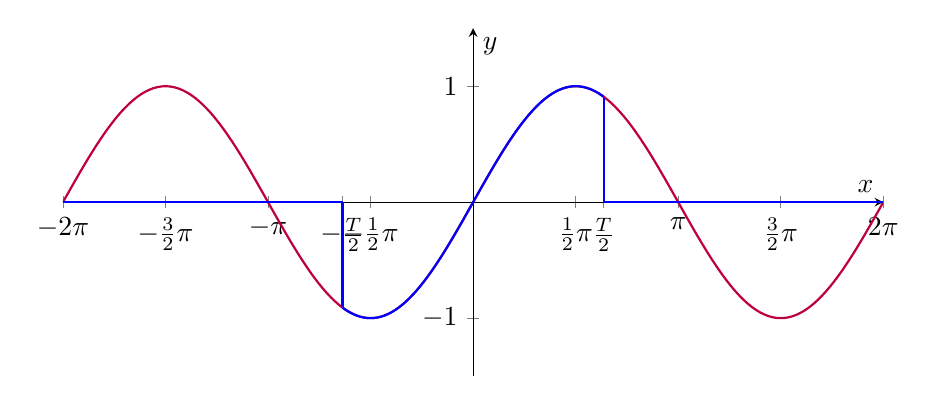
\begin{tikzpicture}
                        \begin{axis}[
                            domain=-2*pi:2*pi,
                            samples=200,
                            axis lines=middle,
                            xlabel=$x$,
                            ylabel=$y$,
                            ymin=-1.5,
                            ymax=1.5,
                            xtick={-2*pi, -3/2*pi, -pi, -1/2*pi,-2, 0, 2,1/2*pi, pi, 3/2*pi, 2*pi},
                            xticklabels={$-2\pi$, $-\frac{3}{2}\pi$, $-\pi$, $-\frac{1}{2}\pi$,$-\frac{T}{2}$, $0$, $\frac{T}{2}$, $\frac{1}{2}\pi$, $\pi$, $\frac{3}{2}\pi$, $2\pi$},
                            ytick={-1, 1},
                            yticklabels={$-1$, $1$},
                            width=12cm,
                            height=6cm
                        ]
                        \addplot [purple, thick] {sin(deg(x))};
                        \addplot [blue, thick, domain = -2:2] {sin(deg(x))};
                        \addplot [blue, thick, domain = 2:2*pi] {0};
                        \addplot [blue, thick, domain = -2*pi:-2] {0};
                        \addplot [const plot, thick,color=blue] coordinates {(-2,-0.9) (-2,0)};
                        \addplot [const plot, thick,color=blue] coordinates {(2,0.9) (2,0)};
                        \end{axis}
                    \end{tikzpicture}
                    \caption{Segnale troncato}
                    \label{fig:troncato}
                \end{figure}
            

            % NON CAPISCO COSA É POTENZA MEDIA E COSA SIA POTENZA ISTANTANEA CHE CAVOLO DI RELAZIONE
            % USO PER PASSARE DA PxT A Px  
            La potenza media é:
            \[
                P_{x_{T}} \triangleq \frac{E_{x_{T}}}{T}    
            \]
            \[
                E_{x_{T}} = \int_{-\frac{T}{2}}^{\frac{T}{2}}  |x_{(t)}|^2 \,dt  
            \]
            dalla quale possiamo ricavare se $T \rightarrow \infty \Rightarrow P_{x_{T}} = P_{x}$:
            \[
                P_{x} \triangleq \lim_{T\rightarrow\infty} \frac{E_{x_{T}}}{T} =\lim_{T\rightarrow\infty} \frac{1}{T} \int_{-\frac{T}{2}}^{\frac{T}{2}}  |x_{(t)}|^2 \,dt    
            \]  
            Possiamo ricavaredelle propietá secondo energia e potenza:
            \begin{itemize}
                \item Se $x_{(t)}$ ha $E_x < \infty \Rightarrow P_x = 0$
                \item Se $x_{(t)}$ ha $P_x = k \neq 0 < \infty \Rightarrow E_x = \infty$
            \end{itemize}
        \subsubsection{Valore Efficace}\label{Valore Efficace}
                \[    
                    x_{eff} \triangleq \sqrt{P_{x}}
                \]
        
        \subsubsection{Valore Medio}\label{Valore medio}

                % TO DO: rivedi qui per evitare un page break
                    \[
                        x_{m} \triangleq \lim_{T\rightarrow\infty} \frac{1}{T} \int_{-\infty}^{\infty}  x_{(t)_T} \,dt = \lim_{T\rightarrow\infty} \frac{1}{T} \int_{-\frac{T}{2}}^{\frac{T}{2}}  x_{(t)} \,dt 
                    \]
                    \[
                        x_{(t)_T}\ =\ Segnale\ troncato
                    \]
                    
    \subsection{Analisi energetiche su segnali comuni}
        \subsubsection{Costante}
            $x_{(t)} = A\ \ \forall t$
            \begin{figure}[h]
                \centering
                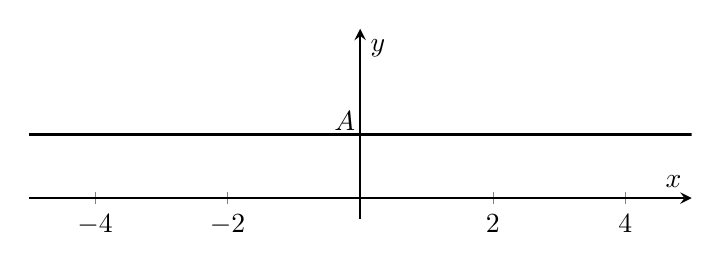
\begin{tikzpicture}
                    \begin{axis}[
                        xlabel=$x$,
                        ylabel=$y$,
                        xmin=-5,
                        xmax=5,
                        ymin=-0.5,
                        ymax=4,
                        ytick = {1.5},
                        yticklabels = {$A$},
                        yticklabel style = {yshift=5pt,xshift=4pt}, 
                        axis lines=middle,
                        thick,
                        domain=-5:5,
                        samples=100,
                        width=10cm,
                        height=4cm
                    ]
                    \addplot [const plot,black, thick] {1.5};
                    \end{axis}
                \end{tikzpicture}
                \caption{Segnale costante}
                \label{fig:segnale costante}
            \end{figure}
            \begin{itemize}
                \item {Energia:
                        \[
                            E_{x} = \int_{-\infty}^{\infty} P_{x}(t) \,dt = \int_{-\infty}^{\infty} |x_{(t)}|^2 \,dt = \int_{-\infty}^{\infty} A^2 \,dt = \infty 
                        \]
                }
                \item {Potenza Media:
                        \[
                            P_{x} = \lim_{T\rightarrow\infty} \frac{E_{x_{T}}}{T} = \lim_{T\rightarrow\infty} \frac{1}{T} \int_{-\frac{T}{2}}^{\frac{T}{2}}  |x_{(t)}|^2 \,dt = \lim_{T\rightarrow\infty} \frac{1}{T} \int_{-\frac{T}{2}}^{\frac{T}{2}} A^2 \,dt = A^2     
                        \]
                }
                \item {Valore Efficace:
                        \[
                            x_{eff} = \sqrt{P_{x}} = \sqrt{A^2} = |A|
                        \]
                }
                \item {Valore Medio:
                        \[
                            x_{m} = \lim_{T\rightarrow\infty} \frac{1}{T} \int_{-\frac{T}{2}}^{\frac{T}{2}}  x_{(t)} \,dt = \lim_{T\rightarrow\infty} \frac{1}{T} \int_{-\frac{T}{2}}^{\frac{T}{2}}  A \,dt = \lim_{T\rightarrow\infty} \frac{1}{T} AT = A 
                        \]
                }
            \end{itemize}
        
        \subsubsection{Cosinusoide}
            $x_{(t)} = A \cos(2 \pi f_0 t +\phi)$\\
            $A = Ampiezza,\  f_0= \frac{1}{T} = frequenza,\ \phi =fase$
            \begin{figure}[H]
                \centering
                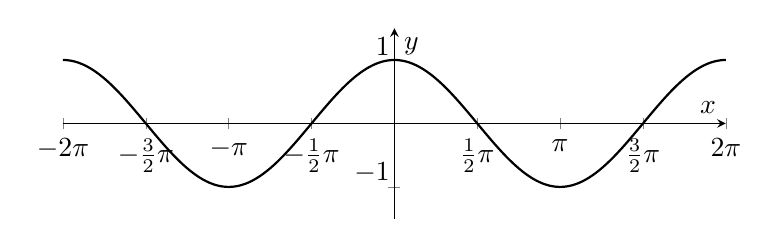
\begin{tikzpicture}
                    \begin{axis}[
                        domain=-2*pi:2*pi,
                        samples=200,
                        axis lines=middle,
                        xlabel=$x$,
                        ylabel=$y$,
                        ymin=-1.5,
                        ymax=1.5,
                        xtick={-2*pi, -3/2*pi, -pi, -1/2*pi, 0,1/2*pi, pi, 3/2*pi, 2*pi},
                        xticklabels={$-2\pi$, $-\frac{3}{2}\pi$, $-\pi$, $-\frac{1}{2}\pi$, $0$, $\frac{1}{2}\pi$, $\pi$, $\frac{3}{2}\pi$, $2\pi$},
                        ytick={-1, 1},
                        yticklabels={$-1$, $1$},
                        yticklabel style = {yshift=5pt,xshift=4pt}, 
                        width=10cm,
                        height=4cm
                    ]
                    \addplot [black, thick] {cos(deg(x))};
                    \end{axis}
                \end{tikzpicture}
                \caption{Segnale cosinusoidale ($\phi = 0$)}
                \label{fig:segnale sinusoidale}
            \end{figure}
            
            \begin{itemize}
                \item {Energia:
                    \[
                        E_{x} = \int_{-\infty}^{\infty} |x_{(t)}|^2 \ dt = \int_{-\infty}^{\infty} A^2 \cos^2(2\pi f_0 t + \phi) dt 
                    \]
                    Ricaviamo dalla $(1)$ \ref{Trigonometria} il $\sin^2(\alpha)$ e lo sostituiamo $(2.1)$ \ref{Trigonometria_Duplicazione} \\ $\cos(2\alpha) = \frac{1+ \cos^2(\alpha)}{2}$
                    \begin{align}
                            &= A^2  \int_{-\infty}^{\infty} \frac{1}{2} + \frac{\cos(4\pi f_0 t + 2\phi)}{2} dt \nonumber \\
                            &= A^2  \int_{-\infty}^{\infty} \frac{1}{2} dt + A^2 \int_{-\infty}^{\infty} \frac{\cos(4\pi f_0 t + 2\phi)}{2} dt \nonumber \\
                            &= \infty +\eval{\frac{A}{2} \frac{1}{4\pi f_0} \sin(4\pi f_0 t) }_{-\infty}^{\infty} = \infty \nonumber
                    \end{align}
                }
                \item {Potenza Media:
                    \begin{align}
                        P_{x} &=\lim_{T\rightarrow\infty}  \frac{1}{T} \int_{-\frac{T}{2}}^{\frac{T}{2}}  |x_{(t)}|^2 \,dt =\lim_{T\rightarrow\infty} \frac{1}{T} \int_{-\frac{T}{2}}^{\frac{T}{2}} A^2 \cos^2(2\pi f_0 t + \phi) dt \nonumber\\
                              &= \lim_{T\rightarrow\infty} \frac{1}{T} \frac{A}{2}T + \lim_{T\rightarrow\infty} \frac{A}{2}\int_{-\frac{T}{2}}^{\frac{T}{2}}\cos(4\pi f_0 t + 2\phi) dt  \nonumber\\
                              &= \frac{A}{2} + \lim_{T\rightarrow\infty} \eval{\frac{A}{2}\frac{1}{4\pi f_0}\sin(4\pi f_0 t + 2\phi)}_{\frac{T}{2}}^{-\frac{T}{2}} = \frac{A^2}{2} \nonumber
                    \end{align}
                }
                \item {Valore Efficace:
                    \[
                        x_{eff} = \sqrt{P_{x}} = \sqrt{\frac{A^2}{2}} =\frac{|A^2|}{\sqrt{2}} 
                    \]
                }
                \item {Valore Medio:
                    \begin{align}
                        x_{m} &= \lim_{T\rightarrow\infty} \frac{1}{T} \int_{-\frac{T}{2}}^{\frac{T}{2}}  x_{(t)} \,dt =\lim_{T\rightarrow\infty} \frac{1}{T} \int_{-\frac{T}{2}}^{\frac{T}{2}}\cos(2\pi f_0 t+\phi) dt \nonumber \\
                              &= \lim_{T\rightarrow\infty} \frac{1}{T}  \eval{\frac{A}{2}\frac{1}{2\pi f_0}\sin(2\pi f_0 t + \phi)}_{\frac{T}{2}}^{-\frac{T}{2}} = 0 \nonumber
                    \end{align}
                }
            \end{itemize}

            %Richimo per il label del formulario $(1)$ e $(2)$ \ref{Trigonometria} 
        \pagebreak
        \subsubsection{Gradino}
        $U_{(t)} = x_{(t)} = 
            \begin{cases}
                1 & t > 0 \\
                0 & t \leq 0  
            \end{cases}
        $
        \begin{figure}[H]
            \centering
            \begin{tikzpicture}
                \begin{axis}[
                    xlabel=$x$,
                    ylabel=$y$,
                    xmin=-5,
                    xmax=5,
                    ymin=-0.5,
                    ymax=4,
                    ytick = {1.5},
                    xtick = {},
                    xticklabels = {},
                    yticklabels = {$A$},
                    yticklabel style = {yshift=5pt,xshift=4pt}, 
                    axis lines=middle,
                    thick,
                    domain=-5:5,
                    samples=100,
                    width=10cm,
                    height=4cm
                ]
                \addplot [const plot,red, thick] coordinates{(0,1.5)(5,1.5)};
                \addplot [const plot,red, thick] coordinates{(0,0)(0,1.5)};
                \addplot [const plot,red, thick] coordinates{(-5,0)(0,0)};
                \end{axis}
            \end{tikzpicture}
            \caption{Segnale gradino}
            \label{fig:segnale gradino}
            
        \end{figure}        

        \begin{itemize}
            \item {Energia:
                \[
                    E_{x} = \int_{-\infty}^{\infty} |x_{(t)}|^2 \ dt = \int_{-\infty}^{\infty} 1\ dt = \infty 
                \]
            }
            \item {Potenza Media:
                \[
                    P_{x} =\lim_{T\rightarrow\infty}  \frac{1}{T} \int_{-\frac{T}{2}}^{\frac{T}{2}}  |U_{(t)}|^2 \,dt =\lim_{T\rightarrow\infty} \frac{1}{T} \int_{-\frac{T}{2}}^{\frac{T}{2}} 1\ dt = \lim_{T\rightarrow\infty} \frac{1}{T} \frac{T}{2} = \frac{1}{2}
                \]
            }
            \item {Valore Efficace:
                \[
                    x_{eff} = \sqrt{P_{x}} = \frac{1}{\sqrt{2}} 
                \]
            }
            \item {Valore Medio:
                    \[x_{m} = \lim_{T\rightarrow\infty} \frac{1}{T} \int_{-\frac{T}{2}}^{\frac{T}{2}}  x_{(t)} \,dt =\lim_{T\rightarrow\infty} \frac{1}{T} \int_{-\frac{T}{2}}^{\frac{T}{2}} 1\ dt = \lim_{T\rightarrow\infty} \frac{1}{T} \frac{T}{2} = \frac{1}{2} \]
            }
        \end{itemize}
        
        \subsubsection{Rettangolo}
        $x_{(t)} = A\hspace{0.1cm}rect\left(\frac{t}{T}\right) =
            \begin{cases}
                A & -\frac{t}{T}\leq t\leq \frac{t}{T}\\
                0 & Altrove 
            \end{cases}
        $
        \begin{figure}[H]
            \centering
            \begin{tikzpicture}
                \begin{axis}[
                    xlabel=$x$,
                    ylabel=$y$,
                    xmin=-5,
                    xmax=5,
                    ymin=-0.5,
                    ymax=4,
                    ytick = {1.5},
                    xtick={-1.5, 0, 1.5},
                    xticklabels={$-\frac{T}{2}$, $0$, $\frac{T}{2}$},
                    yticklabels = {$A$},
                    yticklabel style = {yshift=5pt,xshift=4pt}, 
                    axis lines=middle,
                    thick,
                    domain=-5:5,
                    samples=100,
                    width=10cm,
                    height=4cm
                ]
                \addplot [const plot,red, thick] coordinates{(-1.5,1.5)(1.5,1.5)};
                \addplot [const plot,red, thick] coordinates{(-1.5,0)(-1.5,1.5)};
                \addplot [const plot,red, thick] coordinates{(1.5,0)(1.5,1.5)};
                \addplot [const plot,red, thick] coordinates{(5,0)(1.5,0)};
                \addplot [const plot,red, thick] coordinates{(-5,0)(-1.5,0)};
                \end{axis}
              \end{tikzpicture}
            \caption{Segnale rettangolo}
            \label{fig:segnale rettangolo}
        \end{figure}        
        \begin{itemize}
            \item {Energia:
                \[
                    E_{x} = \int_{-\infty}^{\infty} |x_{(t)}|^2 \ dt = \int_{-\frac{T}{2}}^{\frac{T}{2}} A^2 \hspace{0.1cm}rect^2\left(\frac{t}{T}\right)\ dt = A^2 \int_{-\frac{T}{2}}^{\frac{T}{2}}  1\ dt = A^2 T 
                \]
            }
            \item {Potenza Media:
                $T < T_0$ se non fosse cosí avrei una costante
                \begin{align}
                    P_{x} =\lim_{T\rightarrow\infty}  \frac{1}{T_0} \int_{-\frac{T_0}{2}}^{\frac{T_0}{2}}  |x_{(t)}|^2 \,dt & =\lim_{T\rightarrow\infty} \frac{1}{T_0}\int_{-\frac{T_0}{2}}^{\frac{T_0}{2}} A^2 \hspace{0.1cm}rect^2\left(\frac{t}{T}\right)\ dt \nonumber \\
                         & =\lim_{T\rightarrow\infty} \frac{1}{T_0} A^2 T = 0 \nonumber
                \end{align}
            }
            \item {Valore Efficace:
                \[
                    x_{eff} = \sqrt{P_{x}} = 0 
                \]
            }
            \item {Valore Medio:
                    \begin{align}
                        x_{m} = \lim_{T\rightarrow\infty} \frac{1}{T} \int_{-\frac{T}{2}}^{\frac{T}{2}}  x_{(t)} \,dt & = \lim_{T\rightarrow\infty} \frac{1}{T_0}\int_{-\frac{T_0}{2}}^{\frac{T_0}{2}} A\hspace{0.1cm}rect\left(\frac{t}{T}\right)\ dt \nonumber \\
                        & =\lim_{T\rightarrow\infty} \frac{1}{T_0} A T = 0 \nonumber
                    \end{align}
                    \begin{figure}[H]
                        \centering
                        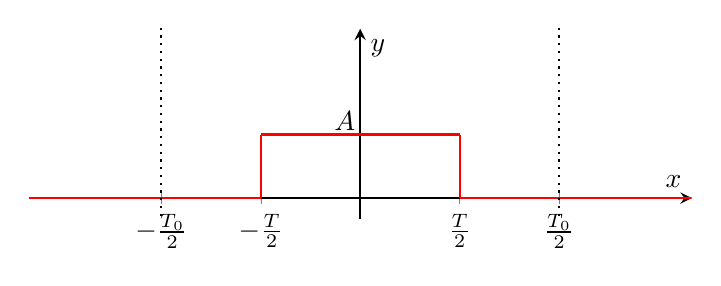
\begin{tikzpicture}
                            \begin{axis}[
                                xlabel=$x$,
                                ylabel=$y$,
                                xmin=-5,
                                xmax=5,
                                ymin=-0.5,
                                ymax=4,
                                ytick = {1.5},
                                xtick={-3,-1.5, 0, 1.5,3},
                                xticklabels={$-\frac{T_0}{2}$,$-\frac{T}{2}$, $0$, $\frac{T}{2}$, $\frac{T_0}{2}$},
                                yticklabels = {$A$},
                                yticklabel style = {yshift=5pt,xshift=4pt}, 
                                axis lines=middle,
                                thick,
                                domain=-5:5,
                                samples=100,
                                width=10cm,
                                height=4cm
                            ]
                            \addplot [const plot,red, thick] coordinates{(-1.5,1.5)(1.5,1.5)};
                            \addplot [const plot,red, thick] coordinates{(-1.5,0)(-1.5,1.5)};
                            \addplot [const plot,red, thick] coordinates{(1.5,0)(1.5,1.5)};
                            \addplot [const plot,red, thick] coordinates{(5,0)(1.5,0)};
                            \addplot [const plot,red, thick] coordinates{(-5,0)(-1.5,0)};
                            \addplot [const plot,dotted, black, thick] coordinates{(3,-5)(3,5)};
                            \addplot [const plot,dotted, black, thick] coordinates{(-3,-5)(-3,5)};
                            \end{axis}
                          \end{tikzpicture}
                        \caption{}
                        \label{fig:segnale rettangolo valore medio}
                    \end{figure}
            }
        \end{itemize}
        
        
        \subsubsection{Esponenziale unilatera}
        $x_{(t)} = e^{-t}U_{(t)}$
        \begin{figure}[H]
            \centering
            \begin{tikzpicture}
                \begin{axis}[
                    xlabel=$x$,
                    ylabel=$y$,
                    xmin=-5,
                    xmax=5,
                    ymin=-0.5,
                    ymax=4,
                    ytick = {1},
                    xtick={},
                    xticklabels={},
                    yticklabels = {$1$},
                    axis lines=middle,
                    thick,
                    domain=-5:5,
                    samples=100,
                    width=10cm,
                    height=4cm
                ]
                \addplot [domain= 0:5,samples = 100,red, thick] {exp(-x)};
                \end{axis}
              \end{tikzpicture}
            \caption{Segnale esponenziale unilatera}
            \label{fig:segnale esponenziale unilatera}
        \end{figure}        
        \begin{itemize}
            \item {Energia:
                \[
                    E_{x} = \int_{-\infty}^{\infty} |x_{(t)}|^2 \ dt = \int_{0}^{\infty} e^{-2t}\ dt = \eval*{\frac{1}{2} e^{-2t}}_{0}^{\infty} = \frac{1}{2} 
                \]
            }
            \item {Potenza Media:
                \begin{align}
                    P_{x} & =\lim_{T\rightarrow\infty}  \frac{1}{T} \int_{-\frac{T}{2}}^{\frac{T}{2}}  |e^{-t}U_{(t)}|^2 \,dt =\lim_{T\rightarrow\infty} \frac{1}{T} \int_{0}^{\frac{T}{2}} e^{-2t}\ dt \nonumber \\
                          & = \lim_{T\rightarrow\infty} \frac{1}{T} \eval*{\left(-\frac{1}{2}\right) e^{-2t}}_{0}^{\frac{T}{2}} =\lim_{T\rightarrow\infty}-\frac{1}{2T} e^{-2\frac{T}{2}} + \lim_{T\rightarrow\infty} \frac{1}{2T} = 0 \nonumber 
                \end{align}
            }
            \item {Valore Efficace:
                \[
                    x_{eff} = \sqrt{P_{x}} = 0 
                \]
            }
            \item {Valore Medio:
                    \begin{align}
                        x_{m} & = \lim_{T\rightarrow\infty} \frac{1}{T} \int_{-\frac{T}{2}}^{\frac{T}{2}}  x_{(t)} \,dt =\lim_{T\rightarrow\infty} \frac{1}{T} \int_{-\frac{T}{2}}^{\frac{T}{2}} e^{-t}U_{(t)}\,dt = \lim_{T\rightarrow\infty} \frac{1}{T} \int_{0}^{\frac{T}{2}} e^{-t}\,dt \nonumber \\
                              & = \lim_{T\rightarrow\infty} \frac{1}{T} \eval*{(-1) e^{-t}}_{0}^{\frac{T}{2}} =  \lim_{T\rightarrow\infty}-\frac{1}{T} e^{-\frac{T}{2}} + \lim_{T\rightarrow\infty} \frac{1}{T} = 0 \nonumber
                    \end{align}
            }
        \end{itemize}
        
        \pagebreak
        \subsubsection{Esponenziale bilatera}
        $x_{(t)} = e^{-|t|}$
        \begin{figure}[H]
            \centering
            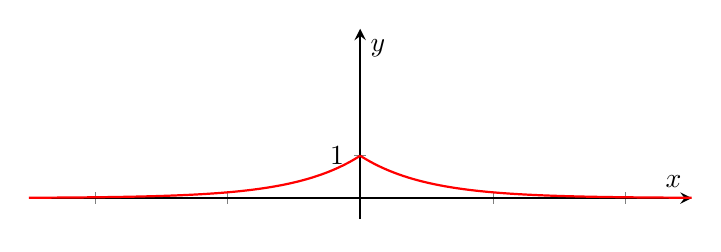
\begin{tikzpicture}
                \begin{axis}[
                    xlabel=$x$,
                    ylabel=$y$,
                    xmin=-5,
                    xmax=5,
                    ymin=-0.5,
                    ymax=4,
                    ytick = {1},
                    xtick={},
                    xticklabels={},
                    yticklabels = {$1$},
                    axis lines=middle,
                    thick,
                    domain=-5:5,
                    samples=100,
                    width=10cm,
                    height=4cm
                ]
                \addplot [domain= 0:5,samples = 100,red, thick] {exp(-x)};
                \addplot [domain= -5:0,samples = 100,red, thick] {exp(x)};
                \end{axis}
              \end{tikzpicture}
            \caption{Segnale esponenziale bilatera}
            \label{fig:segnale esponenziale bilatera}
        \end{figure}        
        \begin{itemize}
            \item {Energia:
                \[
                    E_{x} = \int_{-\infty}^{\infty} |x_{(t)}|^2 \ dt =2 \int_{0}^{\infty} e^{-2t}\ dt = \eval*{2 \left(-\frac{1}{2}\right) e^{-2t}}_{0}^{\infty} = 1 
                \]
            }
            \item {Potenza Media:
                \begin{align}
                    P_{x} & =\lim_{T\rightarrow\infty}  \frac{1}{T} \int_{-\frac{T}{2}}^{\frac{T}{2}}  |e^{-t}U_{(t)}|^2 \,dt =\lim_{T\rightarrow\infty} \frac{2}{T} \int_{0}^{\frac{T}{2}} e^{-2t}\ dt \nonumber \\
                          & = \lim_{T\rightarrow\infty} \frac{1}{T} \eval*{e^{-2t}}_{0}^{\frac{T}{2}} =\lim_{T\rightarrow\infty}-\frac{1}{T} e^{-2\frac{T}{2}} + \lim_{T\rightarrow\infty} \frac{1}{T} = 0 \nonumber 
                \end{align}
            }
            \item {Valore Efficace:
                \[
                    x_{eff} = \sqrt{P_{x}} = 0 
                \]
            }
            \item {Valore Medio:
                    \begin{align}
                        x_{m} & = \lim_{T\rightarrow\infty} \frac{1}{T} \int_{-\frac{T}{2}}^{\frac{T}{2}}  x_{(t)} \,dt =\lim_{T\rightarrow\infty} \frac{1}{T} \int_{-\frac{T}{2}}^{\frac{T}{2}} e^{-t}U_{(t)}\,dt = \lim_{T\rightarrow\infty} \frac{1}{T} 2\int_{0}^{\frac{T}{2}} e^{-t}\,dt \nonumber \\
                              & = \lim_{T\rightarrow\infty} \frac{1}{T} \eval*{(-2) e^{-t}}_{0}^{\frac{T}{2}} =  \lim_{T\rightarrow\infty}-\frac{2}{T} e^{-\frac{T}{2}} + \lim_{T\rightarrow\infty} \frac{2}{T} = 0 \nonumber
                    \end{align}
            }
        \end{itemize}        

        \subsubsection{segno $\mathbf{sgn(x_{(t)})}$}
        $x_{(t)} = sgn(t) =
            \begin{cases}
                -1 & t < 0\\
                1  & t>0 
            \end{cases}
        $
        \begin{figure}[H]
            \centering
            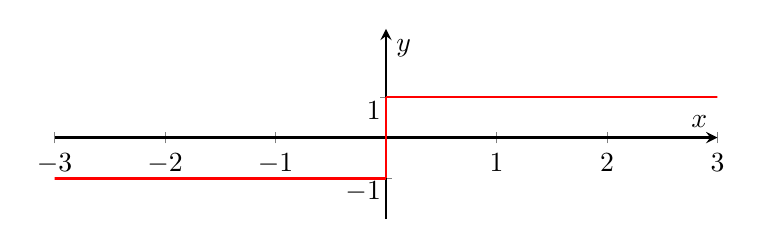
\begin{tikzpicture}
                \begin{axis}[
                    xlabel=$x$,
                    ylabel=$y$,
                    xmin=-3,
                    xmax=3,
                    ymin=-3,
                    ymax=4,
                    ytick={-1.5, 0, 1.5},
                    yticklabels = {$-1$,$0$,$1$},
                    yticklabel style = {yshift=-5pt,xshift=4pt}, 
                    axis lines=middle,
                    thick,
                    domain=-5:5,
                    samples=100,
                    width=10cm,
                    height=4cm
                ]
                \addplot [const plot,red, thick] coordinates{(0,1.5)(5,1.5)};
                \addplot [const plot,red, thick] coordinates{(0,-1.5)(0,1.5)};
                \addplot [const plot,red, thick] coordinates{(0,-1.5)(-5,-1.5)};
                \end{axis}
              \end{tikzpicture}
            \caption{Segnale sgn(x)}
            \label{fig:segnale sgn(x)}
        \end{figure}
        \begin{itemize}
            \item {Energia:
                \[
                    E_{x} = \int_{-\infty}^{\infty} |x_{(t)}|^2 \ dt = \int_{-\infty}^{\infty} sgn^2(t)\ dt = \int_{-\infty}^{\infty} 1\ dt =\infty 
                \]
            }
            \item {Potenza Media:
                \[
                    P_{x} =\lim_{T\rightarrow\infty}  \frac{1}{T} \int_{-\frac{T}{2}}^{\frac{T}{2}}  |x_{(t)}|^2 \,dt =\lim_{T\rightarrow\infty} \frac{1}{T} \int_{-\frac{T}{2}}^{\frac{T}{2}} sgn^2{t}\ dt = \lim_{T\rightarrow\infty} \frac{1}{T} T = 1
                \]
            }
            \item {Valore Efficace:
                \[
                    x_{eff} = \sqrt{P_{x}} = 1 
                \]
            }
            \item {Valore Medio:
                \begin{align}
                    x_{m} & = \lim_{T\rightarrow\infty} \frac{1}{T} \int_{-\frac{T}{2}}^{\frac{T}{2}}  x_{(t)} \,dt =\lim_{T\rightarrow\infty} \frac{1}{T} \int_{-\frac{T}{2}}^{\frac{T}{2}} sgn(t)\ dt \nonumber \\
                          & = \lim_{T\rightarrow\infty} \frac{1}{T} \left[\int_{-\frac{T}{2}}^{0}  1\,dt + \int_{0}^{\frac{T}{2}}  1\,dt\right] = \lim_{T\rightarrow\infty} \frac{1}{T} \left(-\frac{T}{2}+\frac{T}{2}\right) = 0 \nonumber
                \end{align}        
            }
        \end{itemize}
        

    \section{Trasformata Serie Di Fourier}
    \subsection{Segnale Periodico}
        Si definisce segnale periodico un segnale tale che:
        \[
            x_{(t)} = x_{(t-kT_0)}    
        \]
        \[
            T_0=Periodo\ \ \ f_0\triangleq \frac{1}{T_0} =Frequenza
        \]
    \subsection{Trasformata Serie Di Fourier}
        Ogni segnale periodico di periodo $T_0$ che soddifa le condizioni di Dirichlet e la sua $E_x < \infty (C.S.)$ puó essere scritto come la somma di 
        infinite sinusoidi di frequenze multiple di $f_0 = \frac{1}{T_0}$
        \begin{itemize}
            \item{Equazione di Sintesi - Antitrasformata(ATSF)\label{ATSF}
                \[
                    x_{(t)} = \sum_{k = -\infty}^{\infty} X_{k} e^{j2\pi kf_0t} \hspace{1cm} X_{k}\in \mathbb{C},\ f_0 = \frac{1}{T_0} 
                \]
                Se lo sviluppassimo sarebbe composto da:
                \[
                   x_{(t)} =\ldots  + X_{-1} e^{j2\pi (-1)f_0t} + X_{0} + X_{1} e^{j2\pi (1) f_0t} + \ldots 
                \]
                $X_0$ corrisponde al Valore medio \ref{Valore medio} del segnale, inoltre le componenti $X_k$ prendono il nome di armoniche alla frequenza $f$ corrispondente
            }
            \item{Equazione di Analisi - Trasformata(TSF)\label{TSF}
                \[
                    X_k =\frac{1}{T_0}\int_{-\frac{T_0}{2}}^{\frac{T_0}{2}} x_{(t)} e^{-j2\pi kf_0t} dt
                \]
            } 
        \end{itemize}
        La TSF gode della biunivocitá: $\forall x_{(t)} \exists! X_k$:
        \begin{align}
            x_{(t)} & \overunderset{TSF}{ATSF}{\rightleftharpoons} X_k  \nonumber\\
            Segnale\ Analogico\ Periodico &\overunderset{TSF}{ATSF}{\rightleftharpoons} Sequenza\ Complessa \nonumber
        \end{align}
        \subsubsection{Rappresentazione di $X_k$}
            Essendo $X_k$ un numero complesso puó essere rappresentato in forma polare: 
            \[
                X_k = |X_k|e^{\angle X_k}  
            \]
            Si possono rappresentare il modulo (Ampiezza) e la fase tramite grafici che prendono il nome di spettri:
            \begin{figure}[H]
                \centering
                \subfloat[Spettro di Ampiezza]{
                    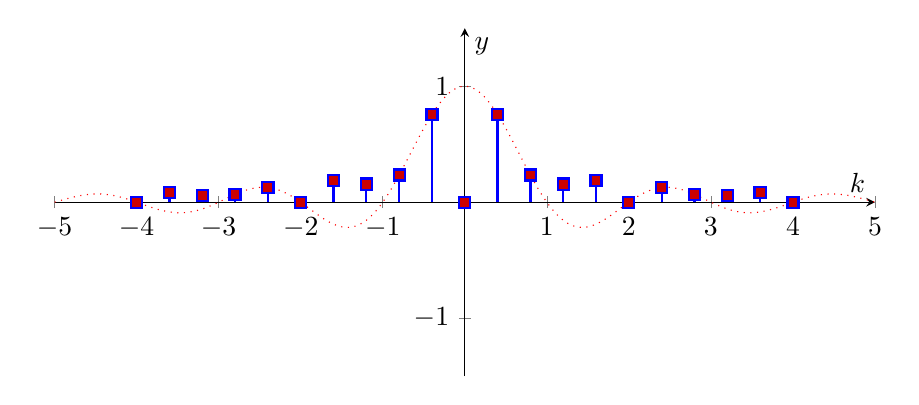
\begin{tikzpicture}
                        \begin{axis}[
                            domain=-5:5,
                            samples=200,
                            axis lines=middle,
                            xlabel=$k$,
                            ylabel=$y$,
                            ymin=-1.5,
                            ymax=1.5,
                            xtick={-5,-4,-3,-2,-1,0,1,2,3,4,5},
                            xticklabels={$-5$,$-4$,$-3$,$-2$,$-1$,$0$,$1$,$2$,$3$,$4$,$5$},
                            ytick={-1, 1},
                            yticklabels={$-1$, $1$},
                            width=12cm,
                            height=6cm
                        ]
                        \addplot [red,dotted, samples = 300] {sin(deg(x*pi))/(x*pi)};
                        \addplot+ [blue, thick, ycomb, samples at={-4,-3.6,-3.2,-2.8,-2.4,-2,-1.6,-1.2,-0.8,-0.4,0,0.4,0.8,1.2,1.6,2,2.4,2.8,3.2,3.6,4}] {abs(sin(deg(x*pi))/(x*pi))};
                        \end{axis}
                    \end{tikzpicture}
                }
                \hfill
                \subfloat[Spettro di Fase]{
                    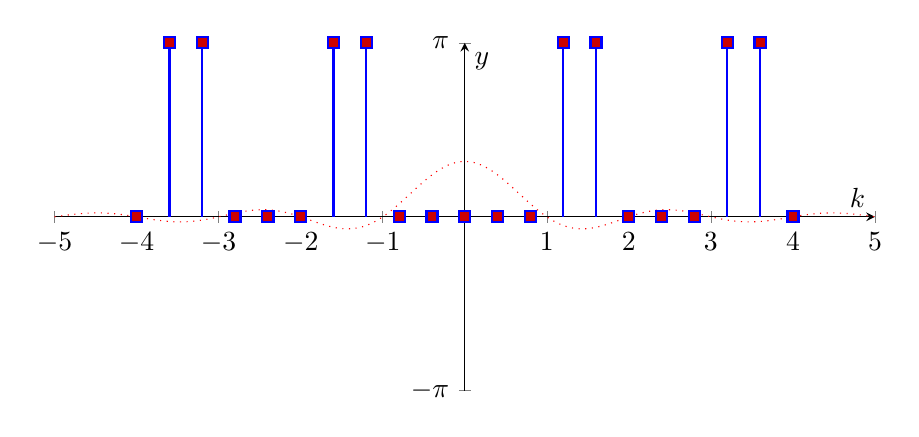
\begin{tikzpicture}
                        \begin{axis}[
                            domain=-5:5,
                            samples=200,
                            axis lines=middle,
                            xlabel=$k$,
                            ylabel=$y$,
                            ymin=-pi,
                            ymax=pi,
                            xtick={-5,-4,-3,-2,-1,0,1,2,3,4,5},
                            xticklabels={$-5$,$-4$,$-3$,$-2$,$-1$,$0$,$1$,$2$,$3$,$4$,$5$},
                            ytick={-pi, pi},
                            yticklabels={$-\pi$, $\pi$},
                            width=12cm,
                            height=6cm
                        ]
                        \addplot [red,dotted, samples = 300] {sin(deg(x*pi))/(x*pi)};
                        \addplot+ [blue, thick, ycomb, samples at={-4,-3.6,-3.2,-2.8,-2.4,-2,-1.6,-1.2,-0.8,-0.4,0,0.4,0.8,1.2,1.6,2,2.4,2.8,3.2,3.6,4}] {rad(atan2(0,sin(deg(x*pi))/(x*pi)))};
                        \end{axis}
                    \end{tikzpicture}
                }
                \caption{Spettro di un treno di rect}
            \end{figure}
            lo spettro di Ampiezza gode della \textbf{simmetria pari} rispetto alle ascisse quindi é \textbf{sempre positivo}, mentre lo spettro di fase della \textbf{simmetria dispari}.
        \subsection{Propietá della TSF}
            \subsection{Linearitá}
            \subsection{Simmetria Hermitiana}
        
        \subsection{Calcolo dei coefficenti $X_k$ per segnali noti}
            \subsubsection{$A\cos(2\pi f_0 t)$}
                $x_{(t)}=A\cos(2\pi f_0 t), \hspace{0.3cm} A>0$
                \begin{align}
                    ATSF[x_{(t)}] & = ATSF[A\cos(2\pi f_0 t)] \nonumber \\
                        & = ATSF[\frac{A}{2} (e^{j2\pi kf_0t} + e^{-j2\pi kf_0t})] \nonumber 
                \end{align}
                Utilizzando la composizione dei coefficenti $X_k$:
                \begin{align}
                    x_{(t)} & =\ldots  + X_{-1} e^{j2\pi (-1)f_0t} + X_{0} + X_{1} e^{-j2\pi (1) f_0t} + \ldots \nonumber\\
                    Abbiamo:& \nonumber 
                \end{align}
                        \[X_{-1} = \frac{A}{2}\hspace{.3cm} X_{0} = 0\hspace{.3cm} X_{1} = \frac{A}{2}\] 
                Possiamo tracciare lo spettro del segnale:
                \begin{figure}[H]
                    \centering
                    \subfloat[Spettro di Ampiezza]{
                    \begin{tikzpicture}
                        \begin{axis}[
                            domain=-4:4,
                            samples=200,
                            axis lines=middle,
                            xlabel=$t$,
                            ylabel=$y$,
                            ymin=-1.5,
                            ymax=1.5,
                            xtick={-5,-4,-3,-2,-1,0,1,2,3,4,5},
                            xticklabels={$-5$,$-4$,$-3$,$-2$,$-1$,$0$,$1$,$2$,$3$,$4$,$5$},
                            ytick={1},
                            yticklabels={$\frac{A}{2}$},
                            width=6.5cm,
                            height=5cm
                            ]
                            \addplot [const plot,black,dotted] coordinates{(-4,1)(4,1)};
                            \addplot+ [blue, thick, ycomb, samples at = {-1,1}] {1};
                            \end{axis}
                        \end{tikzpicture}
                    }
                    \hfill
                    \subfloat[Spettro di Fase]{
                        \begin{tikzpicture}
                            \begin{axis}[
                                domain=-4:4,
                                samples=200,
                                axis lines=middle,
                                xlabel=$t$,
                                ylabel=$y$,
                                ymin=-pi,
                                ymax=pi,
                                xtick={-5,-4,-3,-2,-1,0,1,2,3,4,5},
                                xticklabels={$-5$,$-4$,$-3$,$-2$,$-1$,$0$,$1$,$2$,$3$,$4$,$5$},
                                ytick={-pi, pi},
                                yticklabels={$-\pi$, $\pi$},
                                width=6.5cm,
                                height=5cm
                            ]
                            \addplot+ [blue, thick, ycomb, samples at = {-4,-3,-2,-1,0,1,2,3,4}] {0};
                            \end{axis}
                        \end{tikzpicture}
                    }
                    \caption{Spettro TSF del coseno $A>0$}
                \end{figure}
            \subsubsection{$A\sin(2\pi f_0 t)$}
                $x_{(t)}=A\sin(2\pi f_0 t), \hspace{0.3cm} A>0$
                \begin{align}
                    ATSF[x_{(t)}] & = ATSF[A\sin(2\pi f_0 t)] \nonumber \\
                        & = ATSF[\frac{A}{2} (e^{j2\pi kf_0t} - e^{-j2\pi kf_0t})] \nonumber 
                \end{align}
                Utilizzando la composizione dei coefficenti $X_k$:
                \begin{align}
                    x_{(t)} & =\ldots  + X_{-1} e^{j2\pi (-1)f_0t} - X_{0} + X_{1} e^{-j2\pi (1) f_0t} + \ldots \nonumber\\
                    Abbiamo:& \nonumber 
                \end{align}
                        \[X_{-1} = -\frac{A}{2j}\hspace{.3cm} X_{0} = 0\hspace{.3cm} X_{1} = \frac{A}{2j}\] 
                \[
                    |X_k|= 
                    \begin{cases}
                            |\frac{A}{2j}| = \frac{A}{2} \hspace{0.5cm} & k= 1\\
                            |-\frac{A}{2j}| = \frac{A}{2} \hspace{0.5cm} & k= -1\\
                            0 \hspace{0.5cm} & altrove  \\
                    \end{cases}
                    \hspace{0.5cm}
                    \angle X_k= 
                    \begin{cases}
                        \angle \frac{A}{2j} = -\frac{\pi}{2} \hspace{0.5cm} & k= 1\\
                        \angle |-\frac{A}{2j}| = \frac{\pi}{2} \hspace{0.5cm} & k= -1\\
                        0 \hspace{0.5cm} & altrove  \\
                    \end{cases}
                    \]
                Possiamo tracciare lo spettro del segnale:
                \begin{figure}[H]
                    \centering
                    \subfloat[Spettro di Ampiezza]{
                        \begin{tikzpicture}
                            \begin{axis}[
                                domain=-4:4,
                                samples=200,
                                axis lines=middle,
                                xlabel=$t$,
                                ylabel=$y$,
                                ymin=-1.5,
                                ymax=1.5,
                                xtick={-5,-4,-3,-2,-1,0,1,2,3,4,5},
                                xticklabels={$-5$,$-4$,$-3$,$-2$,$-1$,$0$,$1$,$2$,$3$,$4$,$5$},
                                ytick={1},
                                yticklabels={$\frac{A}{2}$},
                                width=6.5cm,
                                height=5cm
                                ]
                                \addplot [const plot,black,dotted] coordinates{(-4,1)(4,1)};
                                \addplot+ [blue, thick, ycomb, samples at = {-1,1}] {1};
                                \end{axis}
                            \end{tikzpicture}
                        }
                    \hfill
                    \subfloat[Spettro di Fase]{
                            \begin{tikzpicture}
                                \begin{axis}[
                                    domain=-4:4,
                                    samples=200,
                                    axis lines=middle,
                                    xlabel=$t$,
                                    ylabel=$y$,
                                    ymin=-pi,
                                    ymax=pi,
                                    xtick={-5,-4,-3,-2,-1,0,1,2,3,4,5},
                                    xticklabels={$-5$,$-4$,$-3$,$-2$,$-1$,$0$,$1$,$2$,$3$,$4$,$5$},
                                    ytick={-pi,-1/2*pi,1/2*pi, pi},
                                    yticklabels={$-\pi$,$-\frac{\pi}{2}$,$\frac{\pi}{2}$ $\pi$},
                                    yticklabel style = {xshift=3pt}, 
                                    width=6.5cm,
                                    height=5cm
                                ]
                                \addplot+ [blue, thick,const plot] coordinates{(-1,1/2*pi)(-1,0)};
                                \addplot+ [blue, thick,const plot] coordinates{(1,-1/2*pi)(1,0)};

                                \addplot [black, dotted,const plot] coordinates{(-3,-1/2*pi)(3,-1/2*pi)};
                                \addplot [black, dotted,const plot] coordinates{(-3,1/2*pi)(3,1/2*pi)};
                                \end{axis}
                            \end{tikzpicture}
                        }
                    \caption{Spettro TSF del seno $A>0$}
                \end{figure}
            \subsubsection{Treno di rect}
                $x_R=A\hspace{0.1cm}rect\left(\frac{t}{T}\right)\rightarrow$ Segnale periodico $\rightarrow x_{(t)} = \sum_{-\infty}^{\infty} x_R (t-nT_0)$\\
                $T_0 = periodo$, $T = durata \rightarrow T < T_0$, se cosi non fosse avremmo una costante
                \begin{figure}[H]
                    \centering
                    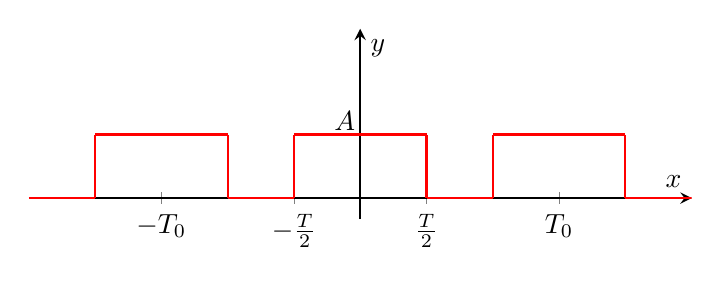
\begin{tikzpicture}
                        \begin{axis}[
                            xlabel=$x$,
                            ylabel=$y$,
                            xmin=-5,
                            xmax=5,
                            ymin=-0.5,
                            ymax=4,
                            ytick = {1.5},
                            xtick={-3,-1, 0, 1,3},
                            xticklabels={$-T_0$,$-\frac{T}{2}$, $0$, $\frac{T}{2}$,$T_0$},
                            yticklabels = {$A$},
                            yticklabel style = {yshift=5pt,xshift=4pt}, 
                            axis lines=middle,
                            thick,
                            domain=-5:5,
                            samples=100,
                            width=10cm,
                            height=4cm
                        ]
                        \addplot [const plot,red, thick] coordinates{(-1,1.5)(1,1.5)};
                        \addplot [const plot,red, thick] coordinates{(-1,0)(-1,1.5)};
                        \addplot [const plot,red, thick] coordinates{(1,0)(1,1.5)};
                        
                        \addplot [const plot,red, thick] coordinates{(-2,1.5)(-4,1.5)};
                        \addplot [const plot,red, thick] coordinates{(-2,0)(-2,1.5)};
                        \addplot [const plot,red, thick] coordinates{(-4,0)(-4,1.5)};
                        
                        \addplot [const plot,red, thick] coordinates{(2,1.5)(4,1.5)};
                        \addplot [const plot,red, thick] coordinates{(2,0)(2,1.5)};
                        \addplot [const plot,red, thick] coordinates{(4,0)(4,1.5)};
                        
                        \addplot [const plot,red, thick] coordinates{(2,0)(1,0)};
                        \addplot [const plot,red, thick] coordinates{(-2,0)(-1,0)};
                        \addplot [const plot,red, thick] coordinates{(-4,0)(-5,0)};
                        \addplot [const plot,red, thick] coordinates{(4,0)(5,0)};
                    
                        \end{axis}
                    \end{tikzpicture}
                    \caption{Treno di $A\hspace{0.1cm}rect\left(\frac{t}{T}\right)$}
                    \label{fig:treno di rect}
                \end{figure}                
                $\rightarrow$ Si nota come cambiare il periodi delle funzioni possiamo renderle da aperiodiche a periodiche e viceversa
                \begin{align}
                    ATSF[x_{(t)}] & = ATSF[\sum_{-\infty}^{\infty} x_R (t-nT_0)] \nonumber \\
                        & = \frac{1}{T_0} \int_{-\frac{T_0}{2}}^{\frac{T_0}{2}} x_{(t)} e^{-j2\pi kf_0t} dt = \frac{1}{T_0} \int_{-\frac{T}{2}}^{\frac{T}{2}} x_{(t)} e^{-j2\pi kf_0t} dt \nonumber \\
                        & = \frac{A}{T_0} \int_{-\frac{T}{2}}^{\frac{T}{2}} e^{-j2\pi kf_0t} dt = \eval{\frac{A}{T_0} \frac{1}{j2\pi kf_0} e^{-j2\pi kf_0t}}_{-\frac{T}{2}}^{\frac{T}{2}} \nonumber \\
                        & = \frac{A}{T_0} \frac{e^{-j\pi kf_0T} - e^{j\pi kf_0T}}{j2\pi kf_0} = \frac{A}{T_0} \frac{e^{j\pi kf_0T}-e^{-j\pi kf_0T}}{-j2\pi kf_0} \nonumber \\
                        & = \frac{A\color{purple}{T}}{T_0} \frac{e^{j\pi kf_0T}-e^{-j\pi kf_0T}}{-j2\pi kf_0\color{purple}{T}} = Af_0T sinc(kf_0T) \nonumber 
                \end{align}
                Tracciamo lo spettro per $f_0T<1$:
                \begin{figure}[H]
                    \centering
                    \subfloat[Spettro di Ampiezza]{
                        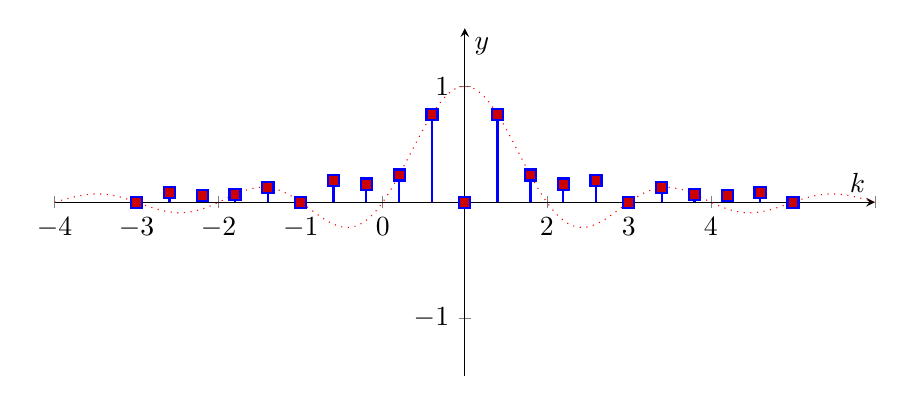
\begin{tikzpicture}
                            \begin{axis}[
                                domain=-5:5,
                                samples=200,
                                axis lines=middle,
                                xlabel=$k$,
                                ylabel=$y$,
                                ymin=-1.5,
                                ymax=1.5,
                                xtick={-5,-4,-3,-2,-1,0,1,2,3,4,5},
                                xticklabels={$-4$,$-3$,$-2$,$-1$,$0$,$1$,$2$,$3$,$4$},
                                ytick={-1, 1},
                                yticklabels={$-1$, $1$},
                                width=12cm,
                                height=6cm
                            ]
                            \addplot [red,dotted, samples = 300] {sin(deg(x*pi))/(x*pi)};
                            \addplot+ [blue, thick, ycomb, samples at={-4,-3.6,-3.2,-2.8,-2.4,-2,-1.6,-1.2,-0.8,-0.4,0,0.4,0.8,1.2,1.6,2,2.4,2.8,3.2,3.6,4}] {abs(sin(deg(x*pi))/(x*pi))};
                            \end{axis}
                        \end{tikzpicture}
                    }
                    \hfill
                    \subfloat[Spettro di Fase]{
                        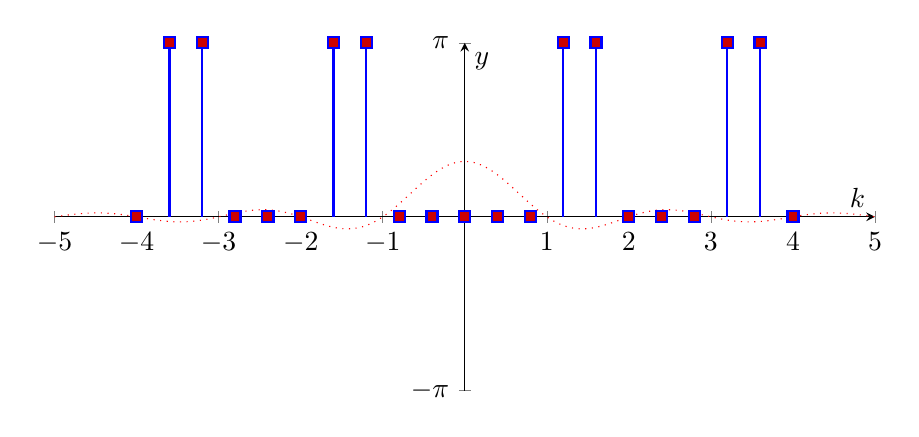
\begin{tikzpicture}
                            \begin{axis}[
                                domain=-5:5,
                                samples=200,
                                axis lines=middle,
                                xlabel=$k$,
                                ylabel=$y$,
                                ymin=-pi,
                                ymax=pi,
                                xtick={-5,-4,-3,-2,-1,0,1,2,3,4,5},
                                xticklabels={$-5$,$-4$,$-3$,$-2$,$-1$,$0$,$1$,$2$,$3$,$4$,$5$},
                                ytick={-pi, pi},
                                yticklabels={$-\pi$, $\pi$},
                                width=12cm,
                                height=6cm
                            ]
                            \addplot [red,dotted, samples = 300] {sin(deg(x*pi))/(x*pi)};
                            \addplot+ [blue, thick, ycomb, samples at={-4,-3.6,-3.2,-2.8,-2.4,-2,-1.6,-1.2,-0.8,-0.4,0,0.4,0.8,1.2,1.6,2,2.4,2.8,3.2,3.6,4}] {rad(atan2(0,sin(deg(x*pi))/(x*pi)))};
                            \end{axis}
                        \end{tikzpicture}
                    }
                    \caption{Spettro TSF del treno di rect con $f_0T<1$}
                \end{figure}
                Si possono anche unire i due spettri per ottenere: 
                \begin{figure}[H]
                    \centering
                    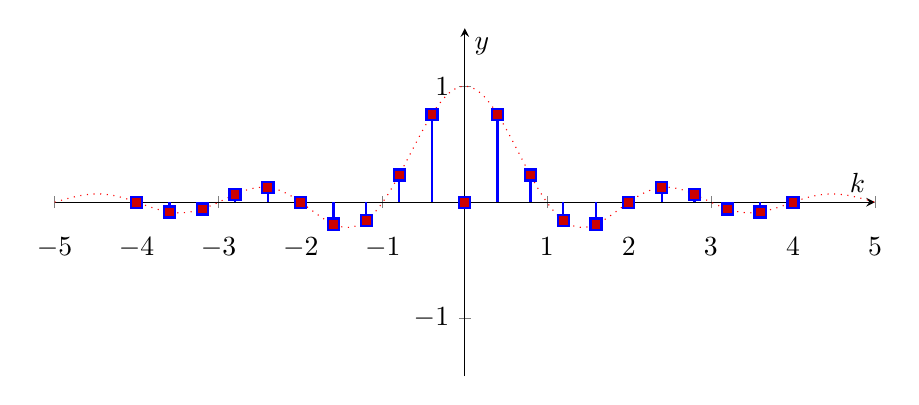
\begin{tikzpicture}
                        \begin{axis}[
                            domain=-5:5,
                            samples=200,
                            axis lines=middle,
                            xlabel=$k$,
                            ylabel=$y$,
                            ymin=-1.5,
                            ymax=1.5,
                            xtick={-5,-4,-3,-2,-1,0,1,2,3,4,5},
                            xticklabels={$-5$,$-4$,$-3$,$-2$,$-1$,$0$,$1$,$2$,$3$,$4$,$5$},
                            ytick={-1, 1},
                            yticklabels={$-1$, $1$},
                            xticklabel style = {yshift=-7pt}, 
                            width=12cm,
                            height=6cm
                        ]
                        \addplot [red,dotted, samples = 300] {sin(deg(x*pi))/(x*pi)};
                        \addplot+ [blue, thick, ycomb, samples at={-4,-3.6,-3.2,-2.8,-2.4,-2,-1.6,-1.2,-0.8,-0.4,0,0.4,0.8,1.2,1.6,2,2.4,2.8,3.2,3.6,4}] {sin(deg(x*pi))/(x*pi)};
                        \end{axis}
                    \end{tikzpicture}
                    \caption{Spettro treno di $A\hspace{0.1cm}rect\left(\frac{t}{T}\right)$}
                    \label{fig:Spettro treno di rect}
                \end{figure}  
            Ora appizza matlab e fa esempi di un segnale e uno di riostruzione dello stesso(script di matlab presenti nel teams):
            \begin{itemize}
                \item Se un segnale varia molto rapidamente nel tempo ha componenti frequenziali piú alte $\rightarrow$ copre piú spettro(espansione spettrale) $T_0 \uparrow$
                \item Se un segnale varia molto lentamente copre le basse fraquenze $ T_0 \downarrow$
            \end{itemize}
            Se non ho abbastanza passi K non posso campionare le alte frequenze e quindi non faccio ne un analisi completa del segnale né riesco a ricostruire perfettametne il segnale  
            Inoltre in $0$ dello spettro ho il Valor medio \ref{Valore medio} del segnale
    \section{Trasformata Continua Di Fourier}
    \subsection{Segnali Aperiodici}
        Nel caso di segnali come $x_{(t)}=rect\left(\frac{t}{T}\right)$ non posso usare la $TSF$ posso peró scrivere:
        \[
            x_{(t)} = \lim_{T_0\rightarrow\infty} x_p(t) ,\ x_p(t) = \sum_{n = -\infty}^{\infty} x_{(t-nT_0)} 
        \]
        Passiamo da un analisi a frequenze discrete ad un analisi su tutto lo spettro delle frequenze
        \begin{figure}[H]
            \centering
            \subfloat[Spettro di Ampiezza TSF]{
                    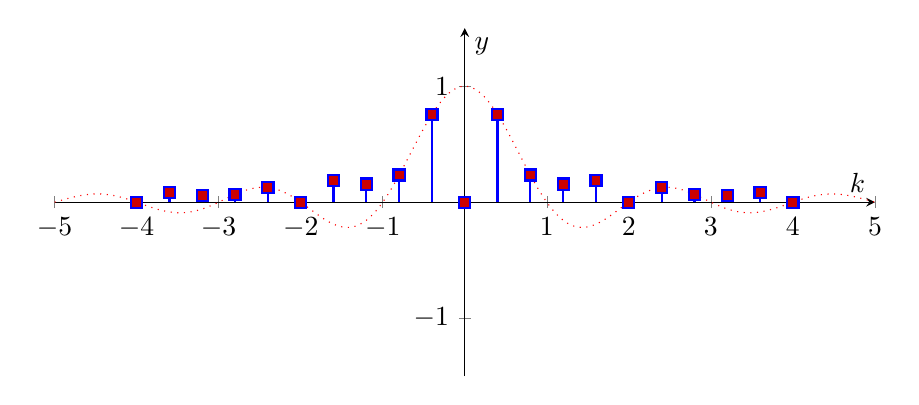
\begin{tikzpicture}
                        \begin{axis}[
                            domain=-5:5,
                            samples=200,
                            axis lines=middle,
                            xlabel=$k$,
                            ylabel=$y$,
                            ymin=-1.5,
                            ymax=1.5,
                            xtick={-5,-4,-3,-2,-1,0,1,2,3,4,5},
                            xticklabels={$-5$,$-4$,$-3$,$-2$,$-1$,$0$,$1$,$2$,$3$,$4$,$5$},
                            ytick={-1, 1},
                            yticklabels={$-1$, $1$},
                            width=12cm,
                            height=6cm
                        ]
                        \addplot [red,dotted, samples = 500] {sin(deg(x*pi))/(x*pi)};
                        \addplot+ [blue, thick, ycomb, samples at={-4,-3.6,-3.2,-2.8,-2.4,-2,-1.6,-1.2,-0.8,-0.4,0,0.4,0.8,1.2,1.6,2,2.4,2.8,3.2,3.6,4}] {abs(sin(deg(x*pi))/(x*pi))};
                        \end{axis}
                    \end{tikzpicture}
                }
                \hfill
                \subfloat[Spettro di Ampiezza TCF]{
                    \begin{tikzpicture}
                        \begin{axis}[
                            domain=-5:5,
                            samples=200,
                            axis lines=middle,
                            xlabel=$f$,
                            ylabel=$y$,
                            ymin=-1.5,
                            ymax=1.5,
                            xtick={-5,-4,-3,-2,-1,0,1,2,3,4,5},
                            xticklabels={$-5$,$-4$,$-3$,$-2$,$-1$,$0$,$1$,$2$,$3$,$4$,$5$},
                            ytick={-1, 1},
                            yticklabels={$-1$, $1$},
                            width=12cm,
                            height=6cm
                        ]
                        \addplot [red,dotted, samples = 300] {sin(deg(x*pi))/(x*pi)};
                        \addplot [blue, thick, samples = 300] {abs(sin(deg(x*pi))/(x*pi))};
                    \end{axis}
                    \end{tikzpicture}
                }
        \end{figure}

    \subsection{Equazioni di Analisi e Sintesi}
        \begin{figure}[H]
            \centering
            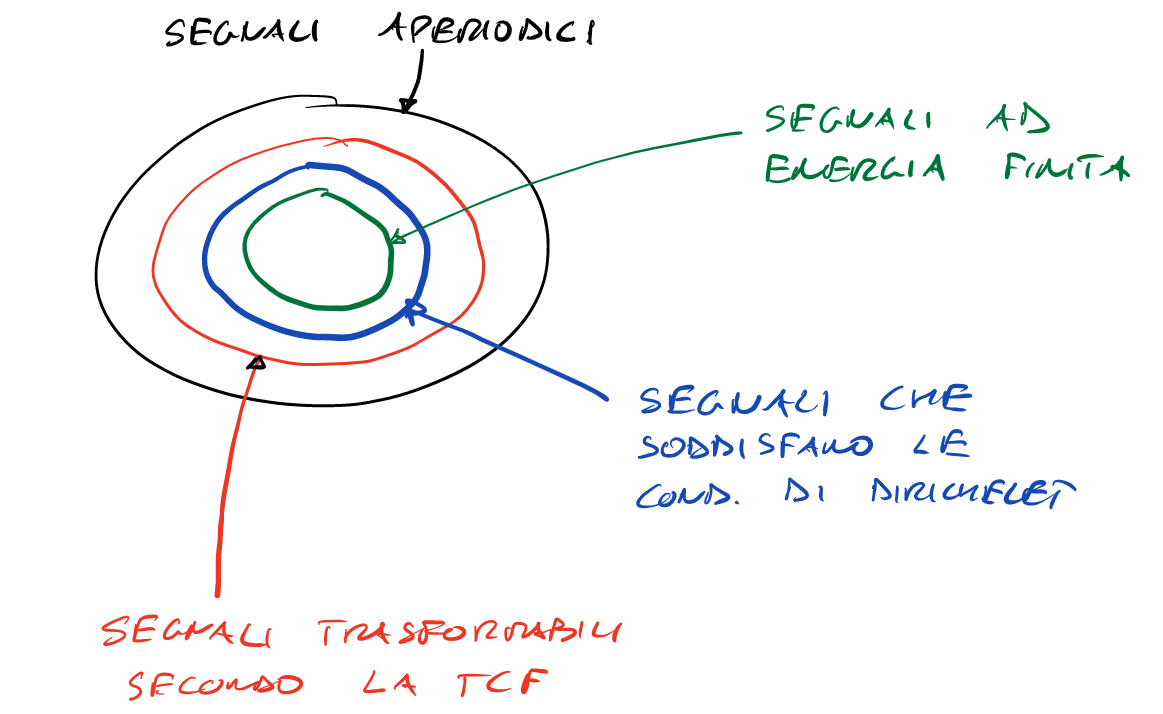
\includegraphics[width=12cm]{media/insiemi_tcf.png}
            \caption{Insiemi dei segnali per tcf}
            \label{fig:segnali aperiodici tcf}
        \end{figure}
        {\subsubsection{Equazione di Analisi}
            \[X_{(f)} = \int_{-\infty}^{\infty} x_{(t)} e^{-j2\pi ft} dt\hspace{0.3cm} Equazione\ di\ analisi \]
            
        \subsubsection{Equazione di Sintesi}
            \[x_{(t)} = \int_{-\infty}^{\infty} X_{(f)} e^{j2\pi ft} df\hspace{0.3cm} Equazione\ di\ sintesi \]
        }
        La $TCF$ gode della biunivocitá
        \begin{align}
            x_{(t)} \rightleftharpoons  X_{(f)}\nonumber \hspace{0.3cm} X_{(f)} \in \mathbb{C}
        \end{align}
        Essendo $X_k$ un numero complesso puó essere rappresentato in forma polare: 
        \[
            X_{(f)} = |X_{(f)}|e^{\angle X_{(f)}}  
        \]
        Si possono rappresentare il modulo (Ampiezza) e la fase tramite grafici che prendono il nome di spettri:
        \begin{figure}[H]
            \centering
            \subfloat[Spettro di Ampiezza]{
                    \begin{tikzpicture}
                        \begin{axis}[
                            domain=-5:5,
                            samples=200,
                            axis lines=middle,
                            xlabel=$f$,
                            ylabel=$y$,
                            ymin=-1.5,
                            ymax=1.5,
                            xtick={-5,-4,-3,-2,-1,0,1,2,3,4,5},
                            xticklabels={$-5$,$-4$,$-3$,$-2$,$-1$,$0$,$1$,$2$,$3$,$4$,$5$},
                            ytick={-1, 1},
                            yticklabels={$-1$, $1$},
                            width=12cm,
                            height=6cm
                        ]
                        \addplot [red,dotted, samples = 300] {sin(deg(x*pi))/(x*pi)};
                        \addplot [blue, thick, samples = 300] {abs(sin(deg(x*pi))/(x*pi))};
                    \end{axis}
                    \end{tikzpicture}
                }
            \hfill
            \subfloat[Spettro di Fase]{
                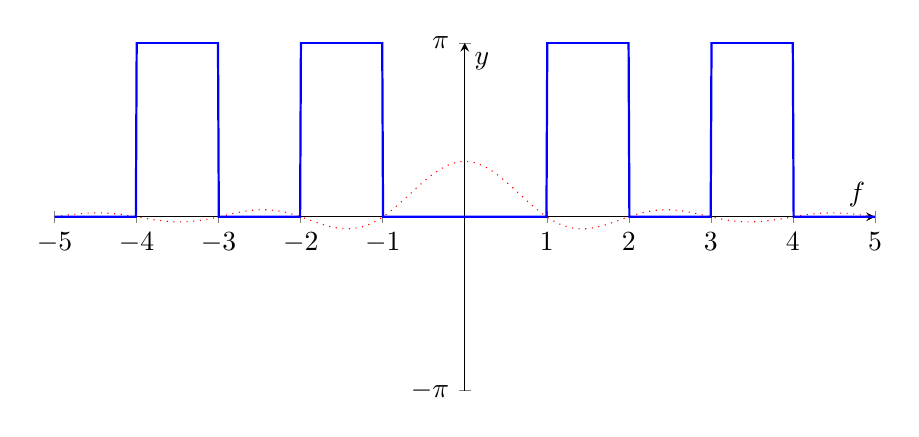
\begin{tikzpicture}
                    \begin{axis}[
                        domain=-5:5,
                        samples=200,
                        axis lines=middle,
                        xlabel=$f$,
                        ylabel=$y$,
                        ymin=-pi,
                        ymax=pi,
                        xtick={-5,-4,-3,-2,-1,0,1,2,3,4,5},
                        xticklabels={$-5$,$-4$,$-3$,$-2$,$-1$,$0$,$1$,$2$,$3$,$4$,$5$},
                        ytick={-pi, pi},
                        yticklabels={$-\pi$, $\pi$},
                        width=12cm,
                        height=6cm
                    ]
                    \addplot [red,dotted, samples = 300] {sin(deg(x*pi))/(x*pi)};
                    \addplot [blue, thick, samples = 1000] {rad(atan2(0,sin(deg(x*pi))/(x*pi)))};
                    \end{axis}
                \end{tikzpicture}
            }
            \caption{Spettro del segnale TCF}
        \end{figure}
        lo spettro di Ampiezza gode della \textbf{simmetria pari} rispetto alle ascisse quindi é \textbf{sempre positivo e continuo}, mentre lo spettro di fase della \textbf{simmetria dispari}, 
        questa propietá é chiamata \textbf{Simmetria Hermitiana}

        \subsubsection{TCF di una $Arect\left(\frac{t}{T}\right)$}
            $x_{(t)} = A\hspace{0.1cm}rect\left(\frac{t}{T}\right)$
            \begin{figure}[H]
                \centering
                \begin{tikzpicture}
                    \begin{axis}[
                        xlabel=$x$,
                        ylabel=$y$,
                        xmin=-5,
                        xmax=5,
                        ymin=-0.5,
                        ymax=4,
                        ytick = {1.5},
                        xtick={-1.5, 0, 1.5},
                        xticklabels={$-\frac{T}{2}$, $0$, $\frac{T}{2}$},
                        yticklabels = {$A$},
                        yticklabel style = {yshift=5pt,xshift=4pt}, 
                        axis lines=middle,
                        thick,
                        domain=-5:5,
                        samples=100,
                        width=8cm,
                        height=4cm
                    ]
                    \addplot [const plot,red, thick] coordinates{(-1.5,1.5)(1.5,1.5)};
                    \addplot [const plot,red, thick] coordinates{(-1.5,0)(-1.5,1.5)};
                    \addplot [const plot,red, thick] coordinates{(1.5,0)(1.5,1.5)};
                    \addplot [const plot,red, thick] coordinates{(5,0)(1.5,0)};
                    \addplot [const plot,red, thick] coordinates{(-5,0)(-1.5,0)};
                    \end{axis}
                  \end{tikzpicture}
                \caption{$A\hspace{0.1cm}rect\left(\frac{t}{T}\right)$}
                \label{fig:grafo rect nella tcf}
            \end{figure}
            $X_{(f)} = ? :$
            \begin{align}
                X_{(f)} & = \int_{-\infty}^{\infty} x_{(t)} e^{-j2\pi ft} dt \nonumber = \int_{-\frac{T}{2}}^{\frac{T}{2}} A\hspace{0.1cm}rect\left(\frac{t}{T}\right) e^{-j2\pi ft} dt \nonumber\\ 
                        & = A \int_{-\frac{T}{2}}^{\frac{T}{2}} e^{-j2\pi ft} dt = -\frac{A}{j2\pi f} \eval{e^{-j2\pi ft}}_{-\frac{T}{2}}^{\frac{T}{2}} =-\frac{A}{j2\pi f} \left(e^{-j\pi fT} - e^{j\pi fT}\right) \nonumber\\
                        & = \frac{A\color{purple}{T}}{\pi f} \left(\frac{e^{j\pi fT} - e^{-j\pi fT}}{2j}\right) = \frac{A{\color{purple}T}\sin(\pi fT)}{\pi f\color{purple}{T}} = AT sinc(fT) =  X_{(f)} \nonumber 
            \end{align}
            \[
                A\hspace{0.1cm}rect\left(\frac{t}{T}\right) \rightleftharpoons AT sinc(fT)
            \]
            La sinc si annulla in $\frac{k}{T},\ k\in \mathbb{Z}$. Notiamo anche come la funzione di partenza sia reale e pari la TCF rispetti \ref{Parita}(si?):
            \begin{figure}[H]
                \centering

            \subfloat[Spettro di Ampiezza]{
                \begin{tikzpicture}
                    \begin{axis}[
                        domain=-5:5,
                        samples=200,
                        axis lines=middle,
                        xlabel=$f$,
                        ylabel=$y$,
                        ymin=-1.5,
                        ymax=1.5,
                        xtick={-5,-4,-3,-2,-1,0,1,2,3,4,5},
                        xticklabels={$-\frac{5}{T}$,$-\frac{4}{T}$,$-\frac{3}{T}$,$-\frac{2}{T}$,$-\frac{1}{T}$,$0$,$\frac{1}{T}$,$\frac{2}{T}$,$\frac{3}{T}$,$\frac{4}{T}$,$\frac{5}{T}$},
                        ytick={-1, 1},
                        yticklabels={$-1$, $1$},
                        width=12cm,
                        height=6cm
                    ]
                    \addplot [red,dotted, samples = 300] {sin(deg(x*pi))/(x*pi)};
                    \addplot [blue, thick, samples = 300] {abs(sin(deg(x*pi))/(x*pi))};
                \end{axis}
                \end{tikzpicture}
                }
            \hfill
            \subfloat[Spettro di Fase]{
                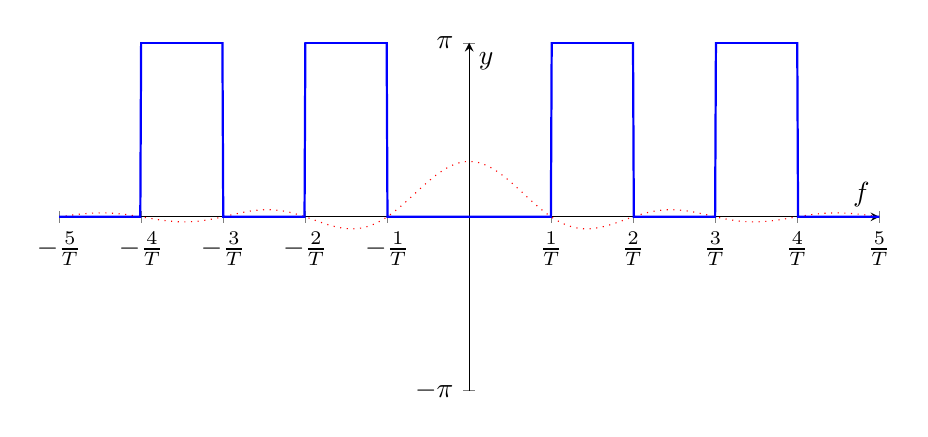
\begin{tikzpicture}
                    \begin{axis}[
                        domain=-5:5,
                        samples=200,
                        axis lines=middle,
                        xlabel=$f$,
                        ylabel=$y$,
                        ymin=-pi,
                        ymax=pi,
                        xtick={-5,-4,-3,-2,-1,0,1,2,3,4,5},
                        xticklabels={$-\frac{5}{T}$,$-\frac{4}{T}$,$-\frac{3}{T}$,$-\frac{2}{T}$,$-\frac{1}{T}$,$0$,$\frac{1}{T}$,$\frac{2}{T}$,$\frac{3}{T}$,$\frac{4}{T}$,$\frac{5}{T}$},
                        ytick={-pi, pi},
                        yticklabels={$-\pi$, $\pi$},
                        width=12cm,
                        height=6cm
                    ]
                    \addplot [red,dotted, samples = 300] {sin(deg(x*pi))/(x*pi)};
                    \addplot [blue, thick, samples = 1000] {rad(atan2(0,sin(deg(x*pi))/(x*pi)))};
                    \end{axis}
                \end{tikzpicture}
            }
            \end{figure}

    \subsection{Propietá}
        Come per la TSF vale che al variare del periodo della funzione $T$:
            \begin{itemize}
                \item Se $T\uparrow$ aumenta $ \rightarrow f\downarrow$ diminuisce e si stringe lo spettro  
                \item Se $T\downarrow$ diminuisce $ \rightarrow f\uparrow$ aumenta e si allarga lo spettro  
            \end{itemize}
        Inoltre come si puó evincere dal successivo Teorema della Dualitá \ref{Dualita}:
            \begin{itemize}
                \item Una funzione limitata (finita) nel tempo ha uno spettro nella frequenza illimitato $\rightarrow$ sono i segnali fisici   
                \item Una funzione illimitata nel tempo ha uno spettro nella frequenza limitato (finito)
            \end{itemize}

        \subsubsection{Simmetria hermitiana}\label{Simmetria Hermitiana}
            \begin{align}
                Ip&: x_{(t)}\ reale \nonumber \\
                Th&: X_{(f)}\ hermitiana \nonumber \\ 
                X_{(-f)} &= X_{(f)}^{*} \rightarrow
                    \begin{cases}
                        |X_{(f)}| = |X_{(-f)}| \hspace{0.3cm} & Simmetria\ Pari \\
                        \angle X_{(-f)} = -\angle X_{(f)}\hspace{0.3cm} & Simmetria\ Dispari
                    \end{cases} \nonumber
            \end{align}

        \subsubsection{Paritá}\label{Parita}
            \begin{align}
                Ip&: x_{(t)}\ reale\ e\ pari  \nonumber \\
                Th&: X_{(f)}\ reale\ e\ pari \nonumber  
            \end{align}

        \subsubsection{Disparitá}\label{Disparita}
            \begin{align}
                Ip&: x_{(t)}\ reale\ e\ dispari  \nonumber \\
                Th&: X_{(f)}\ immaginaria\ e\ dispari \nonumber 
            \end{align}

    \subsection{Teoremi relativi alla TCF}
        \subsubsection{Linearitá}\label{Linearita}
            $Ip: x_{(t)} = \alpha x_{1(t)} + \beta x_{2(t)}$\\        
            $Th: X_{(f)} = \alpha X_{1(f)} + \beta X_{2(f)}$\\ 
            Dimostrazione:
            \begin{align}
                X_{(f)} & = \int_{-\infty}^{\infty} (\alpha x_{1(t)} + \beta x_{2(t)}) e^{-j2\pi ft} dt \nonumber \\
                        & = \alpha \int_{-\infty}^{\infty} x_{1(t)} e^{-j2\pi ft} dt + \beta \int_{-\infty}^{\infty}  x_{2(t)} e^{-j2\pi ft} dt  \nonumber \\
                        & = \alpha X_{1(f)} + \beta X_{2(f)} \nonumber
            \end{align}

            Esempio:
                {   
                    \begin{align}
                        x_{(t)} &= A rect\left(\frac{t}{2T}\right) + Brect\left(\frac{t}{T}\right)\nonumber \\   
                        X_{(f)} &= A X_{1(f)} + B X_{2(f)} = 2AT sinc(2Tf) + BT sinc(Tf) \nonumber \\
                        X_{1(f)} &= 
                        \begin{cases}
                            X_{1(f)} = A rect\left(\frac{t}{T^\prime}\right) \rightleftharpoons^{TCF} T^\prime sinc(T^\prime f) \Rightarrow X_{1(f)} =2Tsinc(2Tf) \\
                            T^\prime = 2T
                        \end{cases} \nonumber
                    \end{align}
                    \begin{figure}[H]
                        \centering
                        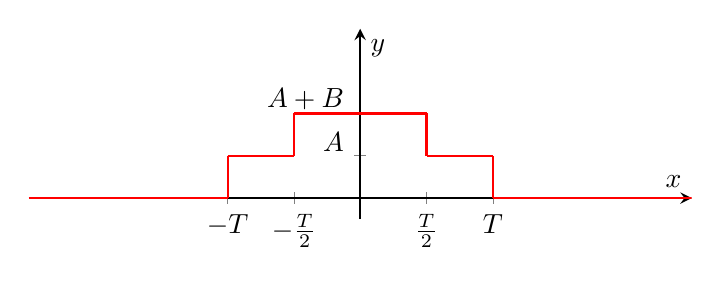
\begin{tikzpicture}
                            \begin{axis}[
                                xlabel=$x$,
                                ylabel=$y$,
                                xmin=-5,
                                xmax=5,
                                ymin=-0.5,
                                ymax=4,
                                ytick = {1,2},
                                yticklabels = {$A$,$A+B$},
                                xtick={-2,-1, 0, 1,2},
                                xticklabels={$-T$,$-\frac{T}{2}$, $0$, $\frac{T}{2}$,$T$},
                                yticklabel style = {yshift=5pt}, 
                                axis lines=middle,
                                thick,
                                domain=-5:5,
                                samples=100,
                                width=10cm,
                                height=4cm
                            ]
                            
                            \addplot [const plot,red, thick] coordinates{(-2,1)(-1,1)};
                            \addplot [const plot,red, thick] coordinates{(2,1)(1,1)};

                            \addplot [const plot,red, thick] coordinates{(1,1)(1,2)};
                            \addplot [const plot,red, thick] coordinates{(-1,1)(-1,2)};
                            \addplot [const plot,red, thick] coordinates{(-1,2)(1,2)};
                            
                            \addplot [const plot,red, thick] coordinates{(-2,0)(-2,1)};
                            \addplot [const plot,red, thick] coordinates{(2,0)(2,1)};


                            \addplot [const plot,red, thick] coordinates{(5,0)(2,0)};
                            \addplot [const plot,red, thick] coordinates{(-5,0)(-2,0)};
                            \end{axis}
                          \end{tikzpicture}
                        \caption{Segnale rettangolo}
                        \label{fig:es linearita}
                    \end{figure}                    
                }
                

        \subsubsection{Dualitá}\label{Dualita}
            $Ip: x_{(t)} \rightleftharpoons^{TCF} X_{(f)}$\\        
            $Th: X_{(t)} \rightleftharpoons^{TCF} x_{(-f)}$ 
            Dimostrazione:
            \begin{align}
                X_{(f)} & = \int_{-\infty}^{\infty} x_{(t)} e^{-j2\pi ft} dt = Sost. \begin{cases}
                    t \rightarrow f\\
                    f \rightarrow t
                \end{cases} \Rightarrow  X_{(t)} = \int_{-\infty}^{\infty} x_{(f)} e^{-j2\pi tf} df \nonumber \\
                        & =Sost.\ (f^\prime = -f) \Rightarrow  X_{(t)} = \int_{-\infty}^{\infty} x_{(-f^\prime)} e^{-j2\pi t(-f^\prime)} df^\prime\nonumber \\
                        & =\int_{-\infty}^{\infty} x_{(-f^\prime)} e^{j2\pi tf^\prime} df^\prime= ACTF[x_{(-f)}] = c.v.d.  \nonumber
            \end{align}
            Esempio:\\
                {
                    $x_{(t)}=Asinc(Bt) \Rightarrow X_{(f)} = \int_{-\infty}^{\infty}A sinc(Bt)e^{-j2\pi ft}dt$ \\
                    Applico la dualitá:
                    \begin{gather}
                        A rect\left(\frac{t}{T}\right) \rightleftarrows ATsinc(Tf) \nonumber \\
                        ATsinc(Tt) \rightleftarrows A rect\left(\frac{-f}{T}\right) \nonumber
                    \end{gather}
                    Se voglio una durata generica:
                    \begin{gather}
                        Sostituisco\ B=T \nonumber \\
                        ABsinc(Bt) \rightleftarrows A rect\left(\frac{f}{B}\right) \nonumber  \\
                        \Downarrow \nonumber \\
                        Asinc(Bt) \rightleftarrows \frac{A}{B}rect\left(\frac{f}{B}\right) \nonumber
                    \end{gather}
                }

        \subsubsection{Ritardo}\label{Ritardo}
            $Ip: x_{(t)} \rightleftharpoons^{TCF} X_{(f)},\ y_{(t)} = x_{(t-to)}$\\        
            $Th: Y_{(f)} \rightleftharpoons^{TCF} y_{(t)} = X_{(f)}e^{-j2\pi ft_0}$\\ 
            Dimostrazione:
            \begin{align}
                Y_{(f)} & = \int_{-\infty}^{\infty} y_{(t)} e^{-j2\pi ft} dt = \int_{-\infty}^{\infty} x_{(t-t_0)} e^{-j2\pi tf} dt \nonumber \\
                        & =Sost.\ (t^\prime = t-t_0) \Rightarrow  Y_{(f)} = \int_{-\infty}^{\infty} x_{(t^\prime)} e^{-j2\pi f(t^\prime+t_0)} dt^\prime \nonumber \\
                        & =\int_{-\infty}^{\infty} x_{(t^\prime)} e^{-j2\pi ft^\prime}e^{-j2\pi ft_0} dt^\prime= X_{(f)}e^{-j2\pi ft_0}\ c.v.d.  \nonumber
            \end{align}
            {\em Osservazione:}
                \begin{itemize}
                    \item Un ritardo nel tempo introduce una componente solo di fase che cresce lienarmente con la frequenza
                    \item Un esponenziale nel tempo introduce un ritardo nel dominio della frequenza $x_{(t)}e^{-j2\pi f_0t} \rightarrowtail X_{(f-f_0)}$, vedi \ref{Modulazione con Esponenziale Complesso}
                \end{itemize}
            Esempio:\\
                {
                    $x_{0(t)} = A rect\left(\frac{t}{T}\right) \rightarrow x_{(t)}=x_{0(t-t_0)}\hspace{0.3cm} t_0 = \frac{T}{2}$
                    \begin{figure}[H]
                        \centering
                        \begin{tikzpicture}
                            \begin{axis}[
                                xlabel=$t$,
                                ylabel=$y$,
                                xmin=-5,
                                xmax=5,
                                ymin=-0.5,
                                ymax=4,
                                ytick = {1.5},
                                yticklabels = {$A$},
                                yticklabel style = {yshift=8pt,xshift=4pt}, 
                                xtick={-1,0,1,2},
                                xticklabels={$-\frac{T}{2}$,$0$,$\frac{T}{2}$,$T$},
                                axis lines=middle,
                                thick,
                                domain=-5:5,
                                samples=100,
                                width=10cm,
                                height=5cm
                            ]
                            
                            \addplot [const plot, blue] coordinates{(-1,1.5)(1,1.5)};
                            \addplot [const plot, blue] coordinates{(-1,0)(-1,1.5)};
                            \addplot [const plot, blue] coordinates{(1,0)(1,1.5)};
                            
                            \addplot [const plot, purple] coordinates{(0,1.5)(2,1.5)};
                            \addplot [const plot, purple] coordinates{(0,0)(0,1.5)};
                            \addplot [const plot, purple] coordinates{(2,0)(2,1.5)};
                            
                            \end{axis}
                        \end{tikzpicture}
                        \caption{{\color{blue}$x_{0(t)}$}, {\color{purple}$x_{(t)}$}}
                        \label{fig:ritardo rect}
                    \end{figure}
                    \[
                        X_{(f)} = X_{0(f)}e^{-j2\pi f\frac{T}{2}} = AT sinc(Tf) e^{-j\pi fT}    
                    \]

                    \begin{figure}[H]
                        \centering
                        \subfloat[Ampiezza con ritardo]{
                            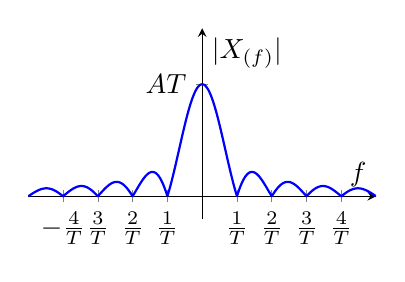
\begin{tikzpicture}
                                \begin{axis}[
                                    domain=-5:5,
                                    samples=200,
                                    axis lines=middle,
                                    xlabel=$f$,
                                    ylabel=$|X_{(f)}|$,
                                    ytick = {1},
                                    yticklabels = {$AT$},
                                    xtick = {-4,-3,-2,-1,0,1,2,3,4},
                                    xticklabels = {$-\frac{4}{T}$,$\frac{3}{T}$,$\frac{2}{T}$,$\frac{1}{T}$,$0$,$\frac{1}{T}$,$\frac{2}{T}$,$\frac{3}{T}$,$\frac{4}{T}$},
                                    ymin=-0.2,
                                    ymax=1.5,
                                    width=6cm,
                                    height=4cm
                                ]
                                \addplot [blue, thick, samples = 500] {abs(sin(deg(x*pi))/(x*pi))};
                                \end{axis}
                            \end{tikzpicture}
                            \label{fig:Ampiezza}
                        }
                        \hfill
                        \subfloat[Fase con ritardo]{
                                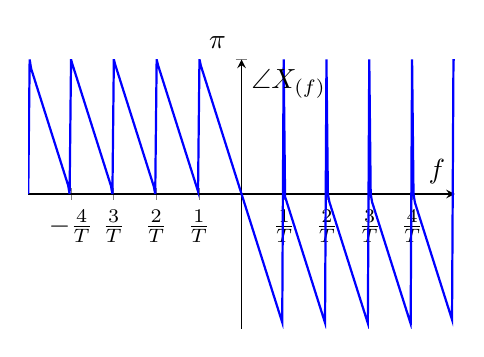
\begin{tikzpicture}
                                    \begin{axis}[
                                        domain=-5:5,
                                        samples=200,
                                        axis lines=middle,
                                        xlabel=$f$,
                                        ylabel=$\angle X_{(f)}$,
                                        ymin=-pi,
                                        ymax=pi,
                                        xtick = {-4,-3,-2,-1,0,1,2,3,4},
                                        xticklabels = {$-\frac{4}{T}$,$\frac{3}{T}$,$\frac{2}{T}$,$\frac{1}{T}$,$0$,$\frac{1}{T}$,$\frac{2}{T}$,$\frac{3}{T}$,$\frac{4}{T}$},
                                        ytick={pi},
                                        yticklabel style = {yshift=6pt}, 
                                        yticklabels={$\pi$},
                                        width=7cm,
                                        height=5cm
                                    ]
                                    \addplot [blue, thick, samples = 300] {rad(atan2((-((sin(deg(pi*x)))^2)/(pi*x)),((cos(deg(pi*x))*sin(deg(pi*x)))/(pi*x))))};
                                    \end{axis}
                                \end{tikzpicture}
                            \label{fig:fase}
                        }
                        \caption{Spettro della $rect$ con ritardo}
                    \end{figure}
                    Il \LaTeX{} sbaglia e aggiunge le spike nelle $f$ positive, il grafico é dispari con andamento come per le $f$ negative.
                }

        \subsubsection{Derivazione}\label{Derivazione}
            $Ip:\begin{cases}
                x_{(t)}\rightleftharpoons^{TCF} X_{(f)}\\
                y_{(t)}= \derivative{}{t} x_{(t)}        
            \end{cases}$\\
            $Th: Y_{(f)} = j2\pi f X_{(f)} $ \\
            Dimostrazione:\\
            \begin{align}
                y_{(t)} &= \derivative{}{t} x_{(t)} = \derivative{}{t} ACTF[x_{(t)}] =\derivative{}{t} \int_{-\infty}^{\infty} X_{(f)}e^{j2\pi ft} df = \nonumber\\
                        &= \int_{-\infty}^{\infty} X_{(f)}\derivative{}{t}e^{j2\pi ft} df = \int_{-\infty}^{\infty} X_{(f)}j2\pi fe^{j2\pi ft} df \nonumber
            \end{align}
            Posso Scrivere $y_{(t)}$ come $ACTF[y_{(t)}] = \int_{-\infty}^{\infty} Y_{(f)}e^{j2\pi ft} df $, se quindi $Y_{(f)} = j2\pi f X_{(f)}$ l'ugaglianza é valida:
            \[
                y_{(t)} =\int_{-\infty}^{\infty} Y_{(f)}e^{j2\pi ft} df
            \]
            L'operazione di derivata nel dominio della frequenza si traduce in una semplice operazione algebrica, nel tempo avrei dovuto calcolare il 
            rapporto incrementale. Per derivare un segnale posso quindi:
            \begin{gather}
                x_{(t)} \rightarrow TCF \rightarrow j2\pi fX_{(f)} \rightarrow ACTF \rightarrow y_{(t)}\nonumber
            \end{gather}
            
        \subsubsection{Integrazione}\label{Integrazione}
            $Ip:\begin{cases}
                x_{(t)} \rightleftharpoons^{TCF} X_{(f)}\ (1)\\
                y_{(t)} = \int_{-\infty}^{t} x_{(\alpha)} d\alpha\ (2) \\
                \int_{-\infty}^{\infty} x_{(t)} dt\ oppure\ \eval*{X_{(f)}}_{f=0} = 0 \ oppure\ y{(+\infty)} = 0\ (3) \\
            \end{cases}$\\
            $Th: Y_{(f)} =\frac{X_{(f)}}{j2\pi f}$ \\
            Dimostrazione:\\
            \begin{gather}
                y_{(t)} = \int_{-\infty}^{t} x_{(\alpha)} d\alpha \Rightarrow {\color{purple}\derivative{}{t}} x_{(t)} = {\color{purple}\derivative{}{t}} y_{(t)} \Rightarrow^{Th. \ref{Derivazione}}  X_{(f)} = j2\pi f Y_{(f)} \nonumber\\
                         Y_{(f)} =\frac{X_{(f)}}{j2\pi f}\nonumber
            \end{gather}

            L'ipotesi 3 é conseguenza della divisione per $f$ e che devo mantenere l'uguaglianza $X_{(f)} = j2\pi f Y_{(f)}$, si nota come nella dimostrazione usando il Th della Derivazione (\ref{Derivazione})
            quando $f=0$ la funzione nella frequenza deve essere $0,\ X_{(f)} = j2\pi f Y_{(f)} = 0$ 
        
        Esempio: $TCF$ di una piramide\\
        {
            \[
                x_{(t)} = A\left(1-\left(\frac{|t|}{T}\right)\right)rect \left(\frac{t}{2T}\right) \hspace{0.3cm} X_{(f)} = TCF[x_{(t)}] = ?
            \]
            \begin{figure}[H]
                \centering
                \begin{tikzpicture}
                    \begin{axis}[
                        xlabel=$t$,
                        ylabel=$x_{(t)}$,
                        xmin=-5,
                        xmax=5,
                        ymin=-0.5,
                        ymax=3,
                        ytick = {2},
                        yticklabels = {$A$},
                        xtick={-2,0,2},
                        xticklabels={$-T$,$0$,$T$},
                        axis lines=middle,
                        thick,
                        domain=-5:5,
                        samples=100,
                        width=10cm,
                        height=5cm
                    ]
                    
                    \addplot [sharp plot, blue] coordinates{(-2,0)(0,2)};
                    \addplot [sharp plot, blue] coordinates{(2,0)(0,2)};
                    \addplot [sharp plot, blue] coordinates{(2,0)(5,0)};
                    \addplot [sharp plot, blue] coordinates{(-2,0)(-5,0)};

                    \end{axis}
                \end{tikzpicture}
                \caption{Funzione priamide}
                \label{fig:funzione piramide}
            \end{figure}
            $TCF[x_{(t)}]:$
            \begin{itemize}
                \item {
                    Utilizzando la classica $TCF$:\\     
                        \[X_{(f)} = \int_{-\infty}^{\infty} A\left(1-\left(\frac{|t|}{T}\right)\right)rect \left(\frac{t}{2T}\right) dt\]
                }
                \item {
                    Utilizzando il Th dell'Integrazione \ref{Integrazione}:\\     
                    \begin{gather}
                        y_{(t)} = \derivative{}{t} x_{(t)} \implies x_{(t)}= \int_{-\infty}^{t} y_{(\alpha)} d\alpha\ \ref{Integrazione}(2) \nonumber \\
                        \int_{-\infty}^{\infty} y_{(t)} dt\ \ref{Integrazione}(3) \nonumber
                    \end{gather}
                    \begin{figure}[H]
                        \centering
                        \begin{tikzpicture}
                            \begin{axis}[
                                xlabel=$t$,
                                ylabel=$x_{(t)}$,
                                xmin=-5,
                                xmax=5,
                                ymin=-3,
                                ymax=3,
                                ytick = {-2,2},
                                yticklabels = {$-\frac{A}{T}$,$\frac{A}{T}$},
                                xtick={-2,-1,0,1,2},
                                xticklabels={$-T$,$-\frac{T}{2}$,$0$,$\frac{T}{2}$,$T$},
                                yticklabel style = {yshift=7pt}, 
                                axis lines=middle,
                                thick,
                                domain=-5:5,
                                samples=100,
                                width=10cm,
                                height=5cm
                            ]
                            
                            \addplot [sharp plot, blue] coordinates{(-2,0)(-2,2)};
                            \addplot [sharp plot, blue] coordinates{(-2,2)(0,2)};

                            \addplot [sharp plot, blue] coordinates{(0,2)(0,-2)};

                            \addplot [sharp plot, blue] coordinates{(0,-2)(2,-2)};
                            \addplot [sharp plot, blue] coordinates{(2,0)(2,-2)};
                            
                            \addplot [sharp plot, blue] coordinates{(-2,0)(-5,0)};
                            \addplot [sharp plot, blue] coordinates{(2,0)(5,0)};
        
                            \end{axis}
                        \end{tikzpicture}
                        \caption{Funzione priamide}
                        \label{fig:derivata piramide}
                    \end{figure}
                    \begin{align}
                        y_{(t)} &= \frac{A}{T}rect \left(\frac{t-\left(-\frac{T}{2}\right)}{T}\right) - \frac{A}{T}rect \left(\frac{t-\frac{T}{2}}{T}\right) = Sono\ 2\ rect\ con\ ritardo \nonumber \\
                                &\Rightarrow y_{(t)} \rightleftharpoons Y_{(f)}\ \ref{Integrazione}(1) \Rightarrow X_{(f)}=\frac{Y_{(f)}}{j2\pi f} 
                                \begin{cases}
                                    x_{(t-t_0)} \rightleftharpoons X_{(f)} e^{-j2\pi ft_0}\nonumber\\
                                    rect \left(\frac{t}{T}\right) \rightleftharpoons Tsinc(Tf) \nonumber
                                \end{cases}\nonumber \\
                        Y_{(f)} &= \frac{A}{T}Tsinc(Tf)e^{-j2\pi f\left(-\frac{T}{2}\right)} - \frac{A}{T}Tsinc(Tf)e^{-j2\pi f\frac{T}{2}} \nonumber\\
                                &= {\color{purple}2j}Asinc(Tf)\frac{e^{j\pi fT}-e^{j\pi fT}}{{\color{purple}2j}} = 2jAsinc(Tf)\sin(\pi fT) \nonumber \\
                        X_{(f)} &= \frac{Y_{(f)}}{j2\pi f} = \frac{2jAsinc(Tf)\sin(\pi fT)}{j2\pi f} = \frac{A{\color{purple}T}sinc(Tf)\sin(\pi fT)}{\pi f{\color{purple}T}}\nonumber\\
                                &= ATsinc^2(fT) \nonumber
                    \end{align}
                    Abbiamo ottenuto la $TCF$ del triangolo:
                    \begin{gather}
                        A\left(1-\left(\frac{|t|}{T}\right)\right)rect \left(\frac{t}{2T}\right) \rightleftharpoons ATsinc^2(fT)\nonumber\\
                        per\ la\ dualita \ref{Dualita}: \nonumber \\
                        ABsinc^2(Bt) \rightleftharpoons A\left(1-\left(\frac{|f|}{B}\right)\right)rect \left(\frac{f}{2B}\right) \nonumber
                    \end{gather} 
                    I segni negativi spariscono per il valore assoluto e per la paritá della $rect$. Per verificare che i calcoli siano
                    corretti posso colacolare la $X_{(f)}$ in $0$ e vedo quanto é l'area del segnale: 
                    \[
                        \eval{T^2sinc(Tf)}_{0} = T^2 \hspace{.2cm} \int_{-\infty}^{\infty} Trect(\frac{t}{T}) = T  
                    \]
                    {\em Osservazione}: la funzione piramidale varia meno rapidamente nel {\em tempo} rispetto alla funzione rettangolare
                    quindi lo spetto non occupa le alte frequenze, l'andamento é di $\frac{sinc^2}{x^2}$, é molto piú contenuto. La rect avendo un gradino
                    varia molto rapidamente nel {\em tempo} e di conseguenza il suo spettro si estende a frequenze piú alte del segnale priamidale.
                    \begin{figure}[H]
                        \centering
                        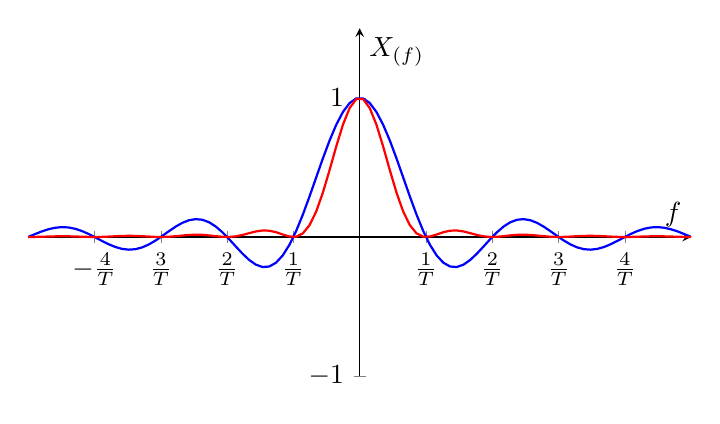
\begin{tikzpicture}
                            \begin{axis}[
                                domain=-5:5,
                                samples=200,
                                axis lines=middle,
                                xlabel=$f$,
                                ylabel=$X_{(f)}$,
                                ytick = {},
                                xtick = {-4,-3,-2,-1,0,1,2,3,4},
                                xticklabels = {$-\frac{4}{T}$,$\frac{3}{T}$,$\frac{2}{T}$,$\frac{1}{T}$,$0$,$\frac{1}{T}$,$\frac{2}{T}$,$\frac{3}{T}$,$\frac{4}{T}$},
                                ymin=-1,
                                ymax=1.5,
                                width=10cm,
                                height=6cm
                            ]
                            \addplot [blue, thick, samples = 100] {sin(deg(x*pi))/(x*pi)};
                            \addplot [red, thick, samples = 100] {(sin(deg(x*pi)))^2/(x*pi)^2};
                            \end{axis}
                        \end{tikzpicture}
                        \caption{{\color{blue}$\frac{sinc}{x}$}, {\color{red}$\frac{sinc^2}{x^2}$}}
                        \label{fig:sinc vs sinc2}
                    \end{figure}
                    DOMANDA: ma la fase in tutto questo che ruolo ha? non avrei problemi avere anche sinc che cambiano la fase degli altri segnali?
                    dopotutto si la sinc é brutta perché si estende all'infinito, ma proprio per questo la fase é sempre sporcata? cosa comporta 
                    nella ricostruzione del segnale? noi abbiamo visto finora l'ampiezza dopotutto
                }
            \end{itemize}
        }
        
        \subsubsection{Derivazione in Frequenza}\label{Derivazione in Frequenza}
            $Ip:\begin{cases}
                x_{(t)}\rightleftharpoons^{TCF} X_{(f)}
                y_{(t)}= \derivative{x_{(t)}}{t}\\        
            \end{cases}$\\
            $Th: Y_{(f)} = j2\pi f X_{(f)} $ \\
            Dimostrazione: ok per ora non l'ha fatta
                
        \subsubsection{Integrazione in Frequenza}\label{Integrazione in Frequenza}
            $Ip:\begin{cases}
                x_{(t)}\rightleftharpoons^{TCF} X_{(f)}
                y_{(t)}= \derivative{x_{(t)}}{t}\\        
            \end{cases}$\\
            $Th: Y_{(f)} = j2\pi f X_{(f)} $ \\
            Dimostrazione: ok per ora non l'ha fatta

                        
        \subsubsection{Convoluzione}\label{Convoluzione}
            \[
                z_{(t)} = x_{(t)} \otimes  y_{(t)} \triangleq \int_{-\infty}^{\infty} x_{(\tau)}y_{(t-\tau)} d\tau
            \] 
            $Ip:\begin{cases}
                x_{(t)}\rightleftharpoons^{TCF} X_{(f)} \\
                x_{(t)}\rightleftharpoons^{TCF} X_{(f)} \\
                z_{(t)} = x_{(t)} \otimes  y_{(t)}   
            \end{cases}$\\
            $Th: Z_{(f)} = X_{(f)}Y_{(f)} $ \\
            Dimostrazione:
                \begin{align}
                    Z_{(f)} &= \int_{-\infty}^{\infty} z_{(t)} e^{-j2\pi ft} dt = \int_{-\infty_{t}}^{\infty}\int_{-\infty_{\tau}}^{\infty} x_{(\tau)}y_{(t-\tau)} e^{-j2\pi ft} dt\ d\tau \nonumber \\
                            &= \int_{-\infty_{t}}^{\infty}x_{(\tau)}\int_{-\infty_{\tau}}^{\infty} y_{(t-\tau)}e^{-j2\pi ft}  dt\ d\tau \Rightarrow^{Th. \ref{Ritardo}} \int_{-\infty}^{\infty}Y_{(f)}x_{(\tau)}e^{-j2\pi f\tau} d\tau  \nonumber \\
                            &= X_{(f)}Y_{(f)} \nonumber
                \end{align}
            Propietá della convoluzione:
            \begin{itemize}
                \item {
                        Commutativa:
                        \[
                            z_{(t)} = x_{(t)} \otimes  y_{(t)} = y_{(t)} \otimes  x_{(t)}  
                        \]
                        Dimostrazione:
                        \begin{align}
                            z_{(t)} &= \int_{-\infty}^{\infty} x_{(\tau)}y_{(t-\tau)} d\tau \Rightarrow \tau=t-\tau^\prime\Rightarrow \int_{-\infty}^{\infty} x_{(t-\tau^\prime)}y_{(\tau^\prime)} d\tau^\prime \nonumber \\
                                    &= \int_{-\infty}^{\infty} y_{(\tau^\prime)}x_{(t-\tau^\prime)} d\tau^\prime = y_{(t)} \otimes  x_{(t)}\nonumber 
                        \end{align}
                    }\label{Conv. Commutativa}
                \item {
                        Associativa:
                        \[
                            (x_{(t)} \otimes  y_{(t)}) \otimes z_{(t)}  =x_{(t)} \otimes  (y_{(t)} \otimes z_{(t)})   
                        \]
                    }\label{Conv. Distributiva}
                \item {
                        Distributiva:
                        \[
                            x_{(t)} \otimes  (y_{(t)}+z_{(t)}) = x_{(t)}\otimes  y_{(t)} +x_{(t)}\otimes  z_{(t)}  
                        \]
                        Dimostrazione:
                        \begin{align}
                            z_{(t)} &= \int_{-\infty}^{\infty} x_{(\tau)}(y_{(t-\tau)}+z_{(t-\tau)}) d\tau = \int_{-\infty}^{\infty}x_{(\tau)}y_{(t-\tau)} +x_{(\tau)}z_{(t-\tau)} d\tau \nonumber \\
                                    &= \int_{-\infty}^{\infty}x_{(\tau)}y_{(t-\tau)} d\tau +\int_{-\infty}^{\infty}x_{(\tau)}z_{(t-\tau)} d\tau = x_{(t)}\otimes  y_{(t)} +x_{(t)}\otimes  z_{(t)} \nonumber 
                        \end{align}
                    }\label{Conv. Associativa}
            \end{itemize}
            Tutte le propietá sono valutate nel dominio del $tempo$ ma valgono anche per il dominio della $frequenza$.
        \subsubsection{Prodotto}\label{Prodotto}
            $Ip:\begin{cases}
                x_{(t)}\rightleftharpoons^{TCF} X_{(f)} \\
                x_{(t)}\rightleftharpoons^{TCF} X_{(f)} \\
                z_{(t)} = x_{(t)}y_{(t)}   
            \end{cases}$\\
            $Th: Z_{(f)} = X_{(f)}\otimes Y_{(f)} $ \\
            Dimostrazione:
                \begin{align}
                    Z_{(f)} &= \int_{-\infty}^{\infty} z_{(t)} e^{-j2\pi ft} dt = \int_{-\infty}^{\infty}x_{(t)}y_{(t)} e^{-j2\pi ft} dt \nonumber \\
                            &= \int_{-\infty_{t}}^{\infty} \int_{-\infty_{\alpha}}^{\infty}X_{(\alpha)}e^{j2\pi \alpha t} d\alpha\ y_{(t)}e^{-j2\pi ft} dt =\int_{-\infty_{\alpha}}^{\infty}X_{(\alpha)} \int_{-\infty_{t}}^{\infty}y_{(t)}e^{-j2\pi (f-\alpha)t} dt\ d\alpha\nonumber \\
                            &\Rightarrow^{\ref{Ritardo}} \int_{-\infty}^{\infty}X_{(\alpha)}Y_{(f-\alpha)}  d\alpha = X_{(f)}\otimes Y_{(f)} \nonumber 
                \end{align}
            \begin{align}
                Tempo&\hspace{1cm} Frequenza \nonumber \\ 
                Convoluzione\ &\Longleftrightarrow \ Prodotto \nonumber \\ 
                Prodotto\ &\Longleftrightarrow \ Convoluzione \nonumber 
            \end{align}
        \subsubsection{Calcolo del prodotto di convoluzione}\label{Calcolo del prodotto di convoluzione}
        \[
            x_{(t)} \otimes  y_{(t)} = \int_{-\infty}^{\infty} x_{(\tau)}y_{(t-\tau)} d\tau \hspace{1cm} y_{(-\alpha)}\ e^\prime\ y_{(\alpha)}\ ruotato 
        \]
        Facciamo un esempio con 2 $rect$:\\

        $x_{(t)} = y_{(t)} = rect\left(\frac{t}{T}\right)$
        \begin{figure}[H]
            \centering
            \subfloat[Grafico nel tempo,{\color{red}$y_{(-\alpha)}$},{\color{blue}$x_{(\alpha)}$}]{
                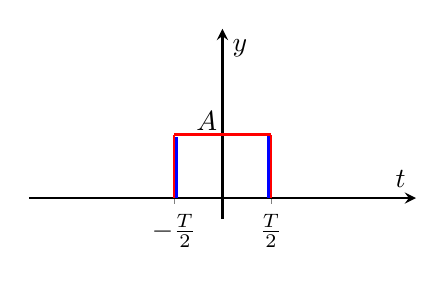
\begin{tikzpicture}
                    \begin{axis}[
                        xlabel=$t$,
                        ylabel=$y$,
                        xmin=-4,
                        xmax=4,
                        ymin=-0.5,
                        ymax=4,
                        ytick = {1.5},
                        xtick={-1, 0, 1},
                        xticklabels={$-\frac{T}{2}$, $0$, $\frac{T}{2}$},
                        yticklabels = {$A$},
                        yticklabel style = {yshift=5pt,xshift=4pt}, 
                        axis lines=middle,
                        thick,
                        domain=-4:4,
                        samples=100,
                        width=6.5cm,
                        height=4cm
                    ]
                    \addplot [const plot, blue, thick] coordinates{(-0.95,1.49)(0.95,1.45)};
                    \addplot [const plot, blue, thick] coordinates{(-0.95,0)(-0.95,1.45)};
                    \addplot [const plot, blue, thick] coordinates{(0.95,0)(0.95,1.45)};
                
                    \addplot [const plot, red, thick] coordinates{(-1,1.5)(1,1.5)};
                    \addplot [const plot, red, thick] coordinates{(-1,0)(-1,1.5)};
                    \addplot [const plot, red, thick] coordinates{(1,0)(1,1.5)};
                
                    \end{axis}
                \end{tikzpicture}
                \label{fig:PC rect}
            }
            \hfill
            \subfloat[illustrazione dell'integrale al variare di $t$,{\color{green}$y_{(t-\alpha)}$},{\color{blue}$x_{(\alpha)}$}]{
                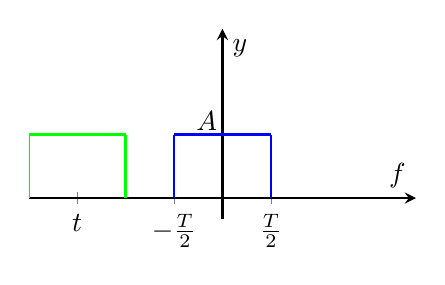
\begin{tikzpicture}
                    \begin{axis}[
                        xlabel=$f$,
                        ylabel=$y$,
                        xmin=-4,
                        xmax=4,
                        ymin=-0.5,
                        ymax=4,
                        ytick = {1.5},
                        xtick={-3,-1, 0, 1},
                        xticklabels={$t$,$-\frac{T}{2}$, $0$, $\frac{T}{2}$},
                        yticklabels = {$A$},
                        yticklabel style = {yshift=5pt,xshift=4pt}, 
                        axis lines=middle,
                        thick,
                        domain=-5:5,
                        samples=100,
                        width=6.5cm,
                        height=4cm
                    ]

                    \addplot [const plot, green, thick] coordinates{(-4,1.5)(-2,1.5)};
                    \addplot [const plot, green, thick] coordinates{(-4,0)(-4,1.5)};
                    \addplot [const plot, green, thick] coordinates{(-2,0)(-2,1.5)};

                    \addplot [const plot, blue, thick] coordinates{(-1,1.5)(1,1.5)};
                    \addplot [const plot, blue, thick] coordinates{(-1,0)(-1,1.5)};
                    \addplot [const plot, blue, thick] coordinates{(1,0)(1,1.5)};
                    \end{axis}
                \end{tikzpicture}
                \label{fig:PC rect in rect}
            }
            \caption{Grafico per il calcolo del prodotto di convoluzione}
        \end{figure}    
        All'aumentare di $t$ {\color{green}$y_{(t-\alpha)}$} si sposta sull'asse delle ascisse, se:
        \begin{itemize}
            \item {
                $t=-\frac{T}{2}$: si allineano le due $rect$ e il valore dell'integrale inizia a aumentare.
            }
            \item {
                $t=0$: si ha il valore massimo del prodotto tra le due funzioni (in questo caso $A=1$), l'integrale vale T.
            }
            \item {
                $t=\frac{T}{2}$: le due $rect$ sono disgiunte, nel raggiungere questa posizione il valore dell'integrale é diminuito fino a $0$.
            }
        \end{itemize}
        Traccamo l'andamento dell'integrale:
        \begin{figure}[H]
            \centering
            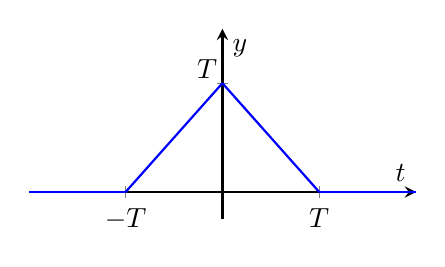
\begin{tikzpicture}
                \begin{axis}[
                    xlabel=$t$,
                    ylabel=$y$,
                    xmin=-4,
                    xmax=4,
                    ymin=-0.5,
                    ymax=3,
                    ytick = {2},
                    xtick={-2, 0, 2},
                    xticklabels={$-T$, $0$, $T$},
                    yticklabels = {$T$},
                    yticklabel style = {yshift=5pt,xshift=4pt}, 
                    axis lines=middle,
                    thick,
                    domain=-4:4,
                    samples=100,
                    width=6.5cm,
                    height=4cm
                ]
                \addplot [sharp plot, blue, thick] coordinates{(-2,0)(0,2)};
                \addplot [sharp plot, blue, thick] coordinates{(2,0)(0,2)};
            
                \addplot [const plot, blue, thick] coordinates{(-2,0)(-4,0)};
                \addplot [const plot, blue, thick] coordinates{(2,0)(4,0)};
            
                \end{axis}
            \end{tikzpicture}
            \label{fig:PC valore integrale}
            \caption{Integrale di convoluzione}
        \end{figure}

        {\em Osservazioni}:
        \begin{itemize}
            \item {Il prodotto di convoluzione ha come durata la somma delle durate dei segnali $[-\frac{T}{2},\frac{T}{2}]\rightarrow[-T,T]$}
            \item {In $t=0$ é l'area il prodotto dei segnali}
        \end{itemize}
        Esempio con $rect$ di durata $T$ e $2T$: 
        \begin{figure}[H]
            \centering
            \subfloat[Grafico delle rect]{
                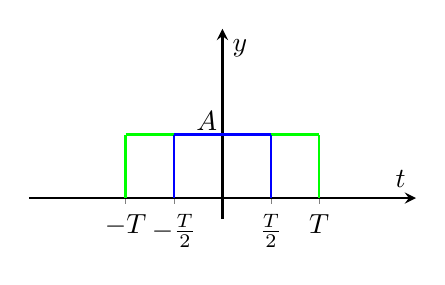
\begin{tikzpicture}
                    \begin{axis}[
                        xlabel=$t$,
                        ylabel=$y$,
                        xmin=-4,
                        xmax=4,
                        ymin=-0.5,
                        ymax=4,
                        ytick = {1.5},
                        xtick={-2,-1, 0, 1,2},
                        xticklabels={$-T$,$-\frac{T}{2}$, $0$, $\frac{T}{2}$,$T$},
                        yticklabels = {$A$},
                        yticklabel style = {yshift=5pt,xshift=4pt}, 
                        axis lines=middle,
                        thick,
                        domain=-4:4,
                        samples=100,
                        width=6.5cm,
                        height=4cm
                    ]
                 
                    \addplot [const plot, green, thick] coordinates{(-2,0)(-2,1.5)};
                    \addplot [const plot, green, thick] coordinates{(2,0)(2,1.5)};
                    \addplot [const plot, green, thick] coordinates{(-2,1.5)(2,1.5)};

                    \addplot [const plot, blue, thick] coordinates{(-1,1.5)(1,1.5)};
                    \addplot [const plot, blue, thick] coordinates{(-1,0)(-1,1.5)};
                    \addplot [const plot, blue, thick] coordinates{(1,0)(1,1.5)};
                    \end{axis}
                \end{tikzpicture}
                \label{fig:PC rect T e 2T}
            }
            \hfill
            \subfloat[Risultato integrale di due $rect$ diverse]{
                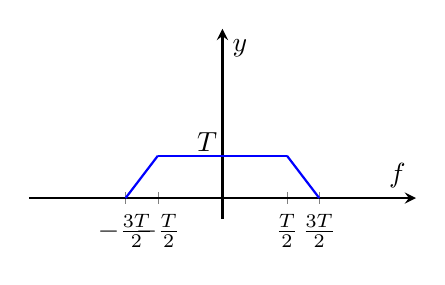
\begin{tikzpicture}
                    \begin{axis}[
                        xlabel=$f$,
                        ylabel=$y$,
                        xmin=-3,
                        xmax=3,
                        ymin=-0.5,
                        ymax=4,
                        ytick = {1},
                        xtick={-3/2,-1, 0,1, 3/2},
                        xticklabels={$-\frac{3T}{2}$,$-\frac{T}{2}$, $0$,$\frac{T}{2}$ ,$\frac{3T}{2}$},
                        yticklabels = {$T$},
                        yticklabel style = {yshift=5pt,xshift=4pt}, 
                        axis lines=middle,
                        thick,
                        domain=-3:3,
                        samples=100,
                        width=6.5cm,
                        height=4cm
                    ]
                        
                    \addplot [sharp plot, blue, thick] coordinates{(-3/2,0)(-1,1)};
                    \addplot [sharp plot, blue, thick] coordinates{(3/2,0)(1,1)};
                    \addplot [sharp plot, blue, thick] coordinates{(-1,1)(1,1)};
                
                    \end{axis}
                \end{tikzpicture}
                \label{fig:PC rect in rect diverse}
            }
            \caption{Integrale di convoluzione di $rect$ di durata diversa}
        \end{figure}
        Esemptio $TCF$ di un triangolo:
        \begin{figure}[H]
            \centering
            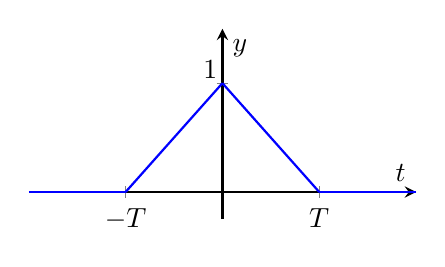
\begin{tikzpicture}
                \begin{axis}[
                    xlabel=$t$,
                    ylabel=$y$,
                    xmin=-4,
                    xmax=4,
                    ymin=-0.5,
                    ymax=3,
                    ytick = {2},
                    xtick={-2, 0, 2},
                    xticklabels={$-T$, $0$, $T$},
                    yticklabels = {$1$},
                    yticklabel style = {yshift=5pt,xshift=4pt}, 
                    axis lines=middle,
                    thick,
                    domain=-4:4,
                    samples=100,
                    width=6.5cm,
                    height=4cm
                ]
                \addplot [sharp plot, blue, thick] coordinates{(-2,0)(0,2)};
                \addplot [sharp plot, blue, thick] coordinates{(2,0)(0,2)};
            
                \addplot [const plot, blue, thick] coordinates{(-2,0)(-4,0)};
                \addplot [const plot, blue, thick] coordinates{(2,0)(4,0)};
            
                \end{axis}
            \end{tikzpicture}
            \label{fig:PC TCF triangolo}
            \caption{Integrale di convoluzione}
        \end{figure}
        Dal Th. di Convoluzione \ref{Convoluzione} sappiamo che é il prodotto di convoluzione di 2 rect di durata uguale a $T$:
        \begin{gather}
            z_{(t)} = x_{(t)}\otimes y_{(t)} = rect\left(\frac{t}{T}\right) \otimes rect\left(\frac{t}{T}\right) \Rightarrow^{\ref{Convoluzione}} Tsinc(fT)\dotproduct Tsinc(fT) \nonumber \\
            T^2sinc(fT) \nonumber 
        \end{gather}
        Esercizio appunti martorella triangoli a sx a dx:
    \subsection{Modulazione di Ampiezza}\label{Modulazione di Ampiezza}
        % \[
        %     y_{(t)} = x_{(t)}\cos(2\pi f_0t)
        % \]
        \begin{figure}[H]
            \centering
            \subfloat[Sistema di modulazione]{
                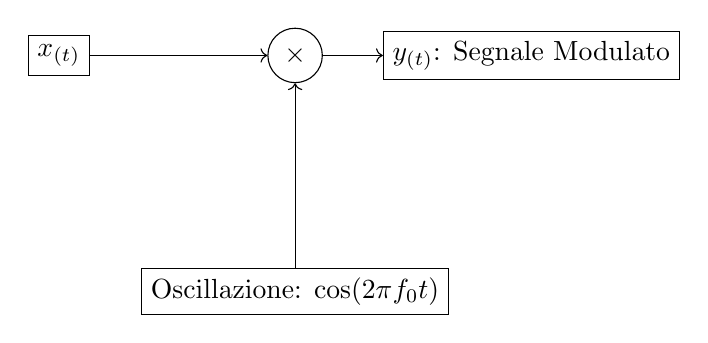
\begin{tikzpicture}[
                        node distance=3cm
                    ]
                    % Blocks
                    \node [rectangle, draw] (input) {$x_{(t)}$};
                    \node [circle, draw, right of=input] (product) {$\times$};
                    \node [rectangle, draw, below of=product] (carrier) {Oscillazione: $\cos(2\pi f_0t)$};
                    \node [rectangle, draw, right of=product] (modulated) {$y_{(t)}$: Segnale Modulato};
                
                    % Connections
                    \draw [->] (input) -- (product);
                    \draw [->] (product) -- (modulated);
                    \draw [->] (carrier) -- (product);
                \end{tikzpicture}    
                \label{fig:sistema di modulazione}
            }
            \hfill
            \subfloat[{\color{blue}$x_{(t)}$}, {\color{red}$y_{(t)}$}, {\color{purple}$\cos (2\pi t)$}]{
                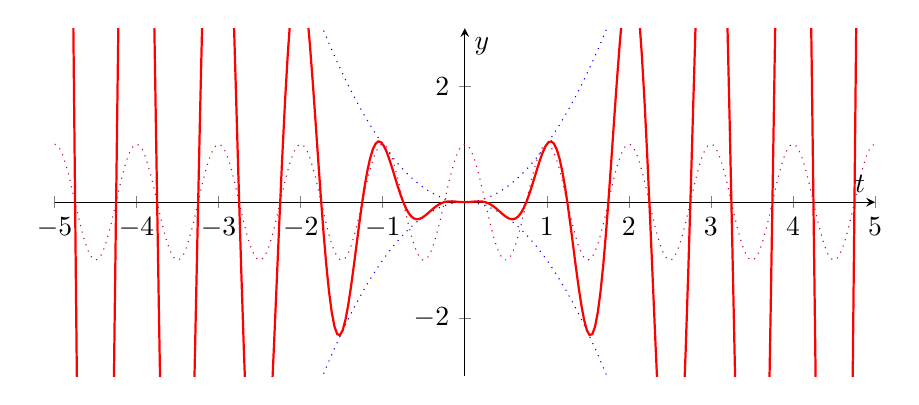
\begin{tikzpicture}
                    \begin{axis}[
                        domain=-5:5,
                        samples=200,
                        axis lines=middle,
                        xlabel=$t$,
                        ylabel=$y$,
                        ymin=-3,
                        ymax=3,
                        width=12cm,
                        height=6cm
                    ]
                    \addplot [blue, dotted, samples = 300] {(x^2)};
                    \addplot [blue, dotted, samples = 300] {-(x^2)};
                    \addplot [purple,dotted, samples = 300] {cos(deg(2*pi*x))};
                    \addplot [red, thick, samples = 300] {cos(deg(2*pi*x))*(x^2)};
                    \end{axis}
                \end{tikzpicture}
                \label{fig:modulazione in ampiezza}
            }
            \caption{Esempio sistema di modulazione di ampiezza}
        \end{figure}
        L'oscillazione introdotta, $\cos (2\pi t)$, segue l'andamento di $x_{(t)}$
        Nel dominio della frequenza:
        \begin{figure}[H]
            \centering
            \subfloat[Senza modulazione]{
                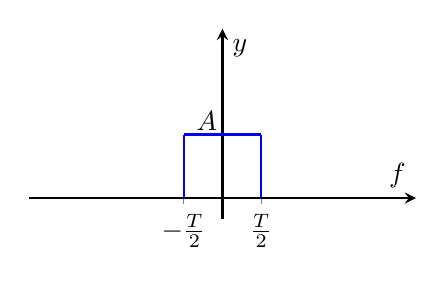
\begin{tikzpicture}
                    \begin{axis}[
                        xlabel=$f$,
                        ylabel=$y$,
                        xmin=-5,
                        xmax=5,
                        ymin=-0.5,
                        ymax=4,
                        ytick = {1.5},
                        xtick={-1, 0, 1},
                        xticklabels={$-\frac{T}{2}$, $0$, $\frac{T}{2}$},
                        yticklabels = {$A$},
                        yticklabel style = {yshift=5pt,xshift=4pt}, 
                        axis lines=middle,
                        thick,
                        domain=-5:5,
                        samples=100,
                        width=6.5cm,
                        height=4cm
                    ]
                    \addplot [const plot, blue, thick] coordinates{(-1,1.5)(1,1.5)};
                    \addplot [const plot, blue, thick] coordinates{(-1,0)(-1,1.5)};
                    \addplot [const plot, blue, thick] coordinates{(1,0)(1,1.5)};
                
                    \end{axis}
                \end{tikzpicture}
                \label{fig:segnale senza modulazione}
            }
            \hfill
            \subfloat[Con modulazione]{
                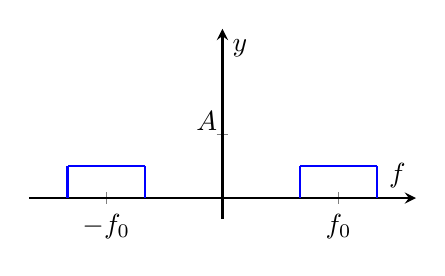
\begin{tikzpicture}
                    \begin{axis}[
                        xlabel=$f$,
                        ylabel=$y$,
                        xmin=-5,
                        xmax=5,
                        ymin=-0.5,
                        ymax=4,
                        ytick = {1.5},
                        xtick={-3,0,3},
                        xticklabels={$-f_0$, $0$,$f_0$},
                        yticklabels = {$A$},
                        yticklabel style = {yshift=5pt,xshift=4pt}, 
                        axis lines=middle,
                        thick,
                        domain=-5:5,
                        samples=100,
                        width=6.5cm,
                        height=4cm
                    ]
                    \addplot [const plot, blue, thick] coordinates{(-2,0.75)(-4,0.75)};
                    \addplot [const plot, blue, thick] coordinates{(-2,0)(-2,0.75)};
                    \addplot [const plot, blue, thick] coordinates{(-4,0)(-4,0.75)};
                    
                    \addplot [const plot, blue, thick] coordinates{(2,0.75)(4,0.75)};
                    \addplot [const plot, blue, thick] coordinates{(2,0)(2,0.75)};
                    \addplot [const plot, blue, thick] coordinates{(4,0)(4,0.75)};
                    
                    \end{axis}
                \end{tikzpicture}
                \label{fig:segnale con modulazione}
            }
            \caption{Segnale nel dominio della frequenza modulato e non}
        \end{figure}
        Serve per spostare la frequenza (es. di trasmissione) del segnale in modo tale, ad esempio, da non sovrapporre due segnali che sono sulla stessa frequenza.
        Se il segnale non fosse modulato si dice in {\color{blue} \textbf{banda base} (BB)} se il segnale é modulato si dice in {\color{red}\textbf{banda passante}(BP)}.
        \begin{figure}[H]
            \centering
            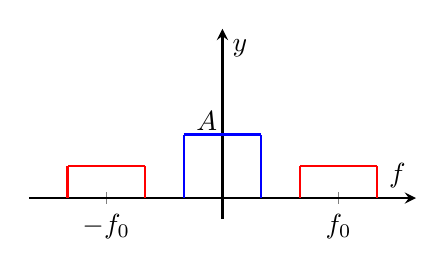
\begin{tikzpicture}
                \begin{axis}[
                    xlabel=$f$,
                    ylabel=$y$,
                    xmin=-5,
                    xmax=5,
                    ymin=-0.5,
                    ymax=4,
                    ytick = {1.5},
                    xtick={-3,0,3},
                    xticklabels={$-f_0$, $0$,$f_0$},
                    yticklabels = {$A$},
                    yticklabel style = {yshift=5pt,xshift=4pt}, 
                    axis lines=middle,
                    thick,
                    domain=-5:5,
                    samples=100,
                    width=6.5cm,
                    height=4cm
                ]
                \addplot [const plot, red, thick] coordinates{(-2,0.75)(-4,0.75)};
                \addplot [const plot, red, thick] coordinates{(-2,0)(-2,0.75)};
                \addplot [const plot, red, thick] coordinates{(-4,0)(-4,0.75)};
                
                \addplot [const plot, red, thick] coordinates{(2,0.75)(4,0.75)};
                \addplot [const plot, red, thick] coordinates{(2,0)(2,0.75)};
                \addplot [const plot, red, thick] coordinates{(4,0)(4,0.75)};
            
                \addplot [const plot, blue, thick] coordinates{(-1,1.5)(1,1.5)};
                \addplot [const plot, blue, thick] coordinates{(-1,0)(-1,1.5)};
                \addplot [const plot, blue, thick] coordinates{(1,0)(1,1.5)};
            
                
                \end{axis}
            \end{tikzpicture}
            \caption{{\color{blue}BB}, {\color{red}BP}}
            \label{fig:bb e bp}
        \end{figure}

        \subsubsection{Th. Modulazione con $\cos(2\pi f_0t)$}\label{Modulazione con coseno}
            $Ip:\begin{cases}
                    y_{(t)}= x_{(t)}\cos(2\pi f_0t)\\        
                    x_{(t)}\rightleftharpoons^{TCF} X_{(f)}
                \end{cases}$\\/usr/share/codium/resources/app/out/vs/code/electron-sandbox/workbench/workbench.html
            $Th: Y_{(f)} = \frac{1}{2} X_{(f-f_0)} + \frac{1}{2} X_{(f+f_0)}$ \\
            Dimostrazione:
            \begin{align}
                Y_{(f)} & = \int_{-\infty}^{\infty} y_{(t)} e^{-j2\pi ft} dt = \int_{-\infty}^{\infty} x_{(t)}\cos(2\pi f_0t) e^{-j2\pi ft} dt \nonumber \\
                & =\int_{-\infty}^{\infty} x_{(t)} \frac{e^{j2\pi f_0t} + e^{-j2\pi f_0t}}{2} e^{-j2\pi ft} dt =  \nonumber \\
                & = \frac{1}{2} \int_{-\infty}^{\infty} x_{(t)} e^{-j2\pi (f-f_0)t} dt + \frac{1}{2} \int_{-\infty}^{\infty} x_{(t)} e^{-j2\pi (f+f_0)t} dt \nonumber \\
                & = \eval{TCF[x_{(t)}]}_{f-f_0} + \eval{TCF[x_{(t)}]}_{f+f_0} = \frac{1}{2} X_{(f-f_0)} + \frac{1}{2} X_{(f+f_0)}\ c.v.d \nonumber  
            \end{align}
            Esempio:\\
            {
                $X_{(f)} = \frac{A}{B}rect\left(\frac{f}{B}\right)$
                \[
                    Y_{(f)} = \frac{A}{2B}rect\left(\frac{f-f_0}{B}\right)+\frac{A}{2B}rect\left(\frac{f+f_0}{B}\right)
                \]
                \begin{figure}[H]
                    \centering
                    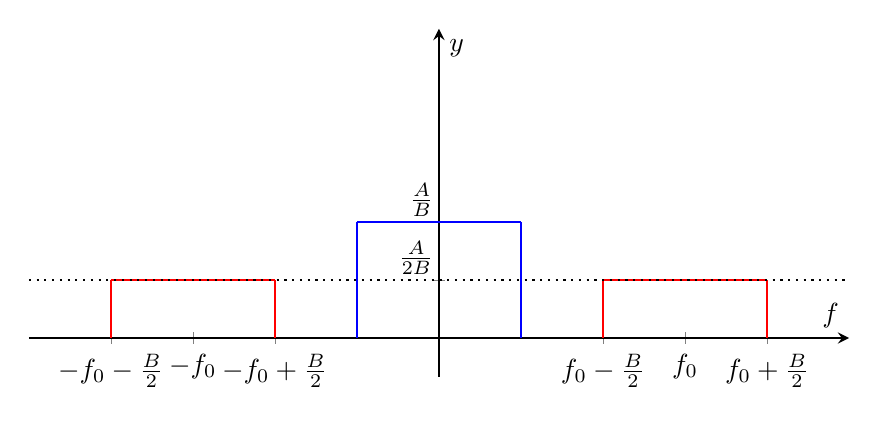
\begin{tikzpicture}
                        \begin{axis}[
                            xlabel=$f$,
                            ylabel=$y$,
                            xmin=-5,
                            xmax=5,
                            ymin=-0.5,
                            ymax=4,
                            ytick = {0.75,1.5},
                            xtick={-4,-3,-2, 0,2,3,4},
                            xticklabels={$-f_0-\frac{B}{2}$,$-f_0$,$-f_0+\frac{B}{2}$,$0$,$f_0-\frac{B}{2}$,$f_0$,$f_0+\frac{B}{2}$},
                            yticklabels = {$\frac{A}{2B}$,$\frac{A}{B}$},
                            yticklabel style = {yshift=8pt,xshift=4pt}, 
                            axis lines=middle,
                            thick,
                            domain=-5:5,
                            samples=100,
                            width=12cm,
                            height=6cm
                        ]
                        \addplot [const plot, red, thick] coordinates{(-2,0.75)(-4,0.75)};
                        \addplot [const plot, red, thick] coordinates{(-2,0)(-2,0.75)};
                        \addplot [const plot, red, thick] coordinates{(-4,0)(-4,0.75)};
                        
                        \addplot [const plot, red, thick] coordinates{(2,0.75)(4,0.75)};
                        \addplot [const plot, red, thick] coordinates{(2,0)(2,0.75)};
                        \addplot [const plot, red, thick] coordinates{(4,0)(4,0.75)};
                    
                        \addplot [const plot, blue] coordinates{(-1,1.5)(1,1.5)};
                        \addplot [const plot, blue] coordinates{(-1,0)(-1,1.5)};
                        \addplot [const plot, blue] coordinates{(1,0)(1,1.5)};
                        
                        \addplot [const plot,dotted, black] coordinates{(-5,0.75)(5,0.75)};

                        \end{axis}
                    \end{tikzpicture}
                    \caption{{\color{blue}$X_{(f)}$}, {\color{red}$Y_{(f)}$}}
                    \label{fig:modulazione rect}
                \end{figure}
            }
            fai cosa ha chiesto lui a fine lezione
        \subsubsection{Th. Modulazione con $\sin(2\pi f_0t)$}\label{Modulazione con seno}
        $Ip:\begin{cases}
                y_{(t)}= x_{(t)}\sin(2\pi f_0t)\\        
                x_{(t)}\rightleftharpoons^{TCF} X_{(f)}
            \end{cases}$\\
        $Th: Y_{(f)} = \frac{1}{2j} X_{(f-f_0)} - \frac{1}{2j} X_{(f+f_0)} $ \\
        Dimostrazione: 
        \begin{align}
            Y_{(f)} & = \int_{-\infty}^{\infty} y_{(t)} e^{-j2\pi ft} dt = \int_{-\infty}^{\infty} x_{(t)}\sin(2\pi f_0t) e^{-j2\pi ft} dt \nonumber \\
            & =\int_{-\infty}^{\infty} x_{(t)} \frac{e^{j2\pi f_0t} - e^{-j2\pi f_0t}}{2j} e^{-j2\pi ft} dt =  \nonumber \\
            & = \frac{1}{2j} \int_{-\infty}^{\infty} x_{(t)} e^{-j2\pi (f-f_0)t} dt - \frac{1}{2j} \int_{-\infty}^{\infty} x_{(t)} e^{-j2\pi (f+f_0)t} dt \nonumber \\
            & = \eval{TCF[x_{(t)}]}_{f-f_0} - \eval{TCF[x_{(t)}]}_{f+f_0} = \frac{1}{2j} X_{(f-f_0)} - \frac{1}{2j} X_{(f+f_0)}\ c.v.d \nonumber  
        \end{align}

        \subsubsection{Th. Modulazione con $\cos(2\pi f_0t + \phi)$}\label{Modulazione con coseno generico}
            $Ip: \begin{cases}
                y_{(t)}= x_{(t)}\cos(2\pi f_0t + \phi)\\        
                x_{(t)}\rightleftharpoons^{TCF} X_{(f)}
                \end{cases}$\\
            $Th: Y_{(f)} = \frac{e^{j\phi}}{2} X_{(f-f_0)} + \frac{e^{-j\phi}}{2} X_{(f+f_0)} $ \\
            Dimostrazione: 
            \begin{align}
                Y_{(f)} & = \int_{-\infty}^{\infty} y_{(t)} e^{-j2\pi ft} dt = \int_{-\infty}^{\infty} x_{(t)}\cos(2\pi f_0t + \phi) e^{-j2\pi ft} dt \nonumber \\
                & =\int_{-\infty}^{\infty} x_{(t)} \frac{e^{j(2\pi f_0t+ \phi)} + e^{-j(2\pi f_0t+ \phi)}}{2} e^{-j2\pi ft} dt =  \nonumber \\
                & = \frac{e^{j\phi}}{2} \int_{-\infty}^{\infty} x_{(t)} e^{-j2\pi (f-f_0)t} dt + \frac{e^{-j\phi}}{2} \int_{-\infty}^{\infty} x_{(t)} e^{-j2\pi (f+f_0)t} dt \nonumber \\
                & = \eval{TCF[x_{(t)}]}_{f-f_0} + \eval{TCF[x_{(t)}]}_{f+f_0} = \frac{e^{j\phi}}{2} X_{(f-f_0)} + \frac{e^{-j\phi}}{2} X_{(f+f_0)}\ c.v.d \nonumber  
            \end{align}
            Esempio:
            \begin{figure}[H]
                \centering
                \subfloat[Ampiezza Mod. generica]{
                    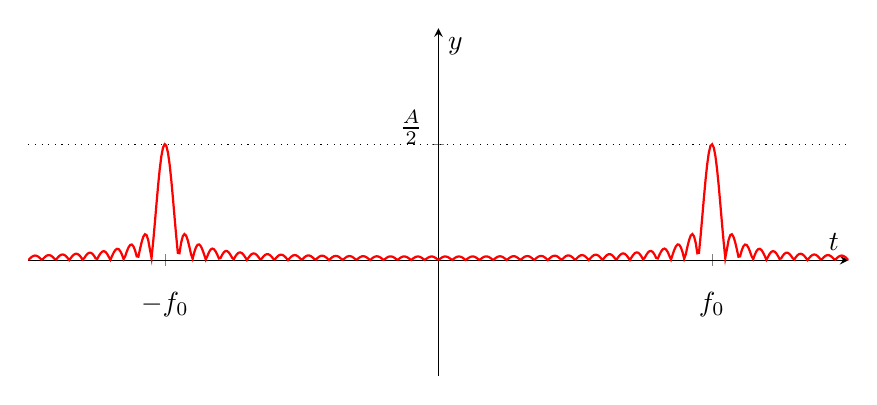
\begin{tikzpicture}
                        \begin{axis}[
                            domain=-30:30,
                            samples=200,
                            axis lines=middle,
                            xlabel=$t$,
                            ylabel=$y$,
                            ytick = {0.5},
                            yticklabels = {$\frac{A}{2}$},
                            yticklabel style = {yshift=6pt},
                            xtick = {-20,20},
                            xticklabels = {$-f_0$,$f_0$},
                            xticklabel style = {yshift=-6pt}, 
                            ymin=-0.5,
                            ymax=1,
                            width=12cm,
                            height=6cm
                        ]
                        \addplot [const plot, dotted,black] coordinates{(-30,0.5)(30,0.5)};
                        \addplot [red, thick, samples = 500] {abs(sin(deg((x-20)*pi))/(2*(x-20)*pi))+abs(sin(deg((x+20)*pi))/(2*(x+20)*pi))};
                        % \addplot [red, thick, samples = 500] {abs(sin(deg((x+20)*pi))/(2*(x+20)*pi))};
                        \end{axis}
                    \end{tikzpicture}
                    \label{fig:Ampiezza Mod. generica}
                }
                \hfill
                \subfloat[fase Mod. generica]{
                        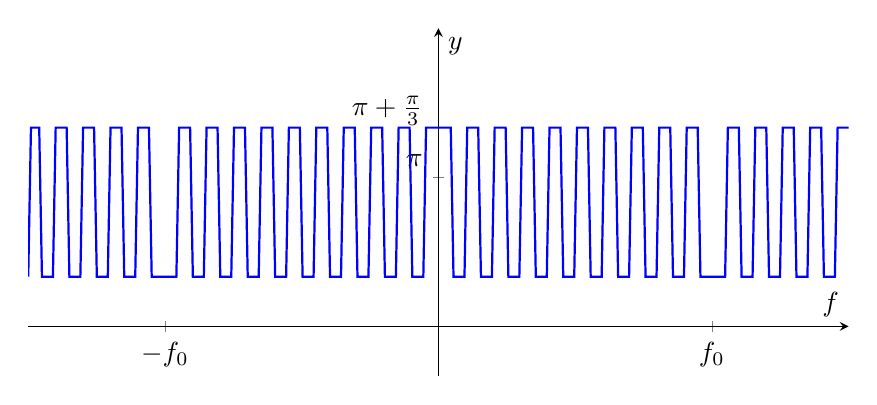
\begin{tikzpicture}
                            \begin{axis}[
                                domain=-30:30,
                                samples=200,
                                axis lines=middle,
                                xlabel=$f$,
                                ylabel=$y$,
                                ymin=-pi/3,
                                ymax=2*pi,
                                xtick={-20,20},
                                xticklabels={$-f_0$,$f_0$},
                                ytick={pi,pi+(pi*1/3)},
                                yticklabel style = {yshift=6pt}, 
                                yticklabels={$\pi$,$\pi+\frac{\pi}{3} $},
                                width=12cm,
                                height=6cm
                            ]
                            \addplot [blue, thick, samples = 300] {rad(atan2(0,(x*sin(deg(pi*x)))/(pi*(-400 + x^2))))+(pi*1/3)};
                            \end{axis}
                        \end{tikzpicture}
                    \label{fig:fase Mod. generica}
                }
                \caption{Modulazione generica di una $A rect\left(\frac{t}{T}\right)$ con $\cos(2\pi f_0t+\frac{\pi}{3})$}
            \end{figure}
        É legale cosa ho scritto sopra della modulazione generica?
        \subsubsection{Th. Modulazione con Esponenziale Complesso}\label{Modulazione con Esponenziale Complesso}
            $Ip: \begin{cases}
                y_{(t)}= x_{(t)}e^{j2\pi f_0t}\\        
                x_{(t)}\rightleftharpoons^{TCF} X_{(f)}
                \end{cases}$\\
            $Th: Y_{(f)} = X_{(f-f_0)} $ \\
            Dimostrazione: 
            \begin{align}
                Y_{(f)} & = \int_{-\infty}^{\infty} y_{(t)} e^{-j2\pi ft} dt = \int_{-\infty}^{\infty} x_{(t)}e^{j2\pi f_0t} e^{-j2\pi ft} dt \nonumber \\
                & =\int_{-\infty}^{\infty} x_{(t)} e^{-j2\pi (f-f_0)t} dt = \eval{TCF[x_{(t)}]}_{f-f_0} = X_{(f-f_0)} \nonumber
            \end{align}
            Posso notare che:
            \begin{itemize}
                \item Ritardo: $\rightarrow x_{(t-t_0)} \rightleftharpoons X_{(f)} e^{(-j2\pi ft_0)}$
                \item Modulazione: $\rightarrow x_{(t)}e^{(j2\pi f_0t)} \rightleftharpoons X_{(f-f_0)}$
            \end{itemize}
            Procedimento per la sintesi di un segnale:
            \begin{itemize}
                \item Derivo il segnale
                \item Verifico le ipotesi del Th. dell'Integrazione \ref{Integrazione}
                \item calcolo la TCF della derivata
                \item Applico il Th. dell'integrazione per calcolare $X_{(f)}$
            \end{itemize}

            \subsubsection{Demodulazione}\label{Demodulazione}
            Ci poniamo il problema di riportare il segnale modulato al segnale originale($g_{(t)}$), dato:\\
            $x_{(t)} = g_{(t)} \cos(2\pi f_0t)$\\
            Demoduliamo il segnale con $2\cos(2\pi f_0t)$:
            \begin{align}
                y_{(t)} &= x_{(t)} {\color{purple}2}\cos(2\pi f_0t) = g_{(t)} \cos^2(2\pi f_0t) \nonumber \\
                        &= g_{(t)} \frac{1+ \cos(4\pi f_0t)}{2} = \frac{g_{(t)}}{2} + \frac{g_{(t)}\cos(4\pi f_0t)}{2}\nonumber\\
                TCF[y_{(t)}] &\Rightarrow^{Th. \ref{Modulazione con coseno}}  \frac{2G_{(f)}}{2} + \frac{2G_{(f-2f_0)}}{2}+ \frac{2G_{(f+2f_0)}}{2} \nonumber \\
                        &= G_{(f)}+G_{(f-2f_0)}+G_{(f+2f_0)}
            \end{align}
            Dall'ultima uguagliaza posso quindi usare un filtro in ({\color{blue}BB}) per rimuovere i segnali alle frequenze $\pm 2f_0$ e ricavare il mio segnale $G_{(f)}$.\\
            DOMANDA: posso anche quindi demodulare con un seno tanto non mi interessa quello che succede alle frequenze spostate,
            quindi peró ritorno sulla fase, non é importante? usando un seno la ribalto praticamente no? ricontroll cio che stai dicendo bro non so 
            se é giusto il ribaltamento \\
            ALTRA DOMANDA: devo anche modulare il segnale abbastanza lontano dalla BB sennó quando demodulo mi autodisturbo il segnale? da qui deriva $\frac{1}{T}<2BB$\\
            ALTRA DOMANDA: quindi se volessi captare piú segnali mi conviene utilizzare circuiti diversi? oppure posso modulare e demodulare a piacimento i segnali tenendo conto 
            su quali frequenze ho modulato in modo tale da sapere dove vanno a finire i segnali e recuperarli? tanto non mi interessa su quale frequenza finiscano finche non diventino 
            non recuperabili per sovrapposizione giusto?\\
            Riporto un po di esempi di demodulazione di una o piú $rect$:
            Esempio di Demodulazione
            \begin{figure}[H]
                \centering
                \subfloat[$sinc$ modulata]{
                    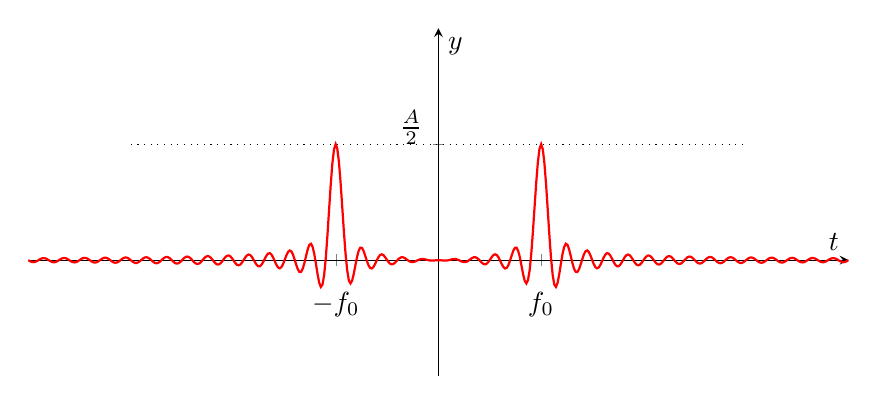
\begin{tikzpicture}
                        \begin{axis}[
                            domain=-40:40,
                            samples=200,
                            axis lines=middle,
                            xlabel=$t$,
                            ylabel=$y$,
                            ytick = {0.5},
                            yticklabels = {$\frac{A}{2}$},
                            yticklabel style = {yshift=6pt},
                            xtick = {-10,10},
                            xticklabels = {$-f_0$,$f_0$},
                            xticklabel style = {yshift=-6pt}, 
                            ymin=-0.5,
                            ymax=1,
                            width=12cm,
                            height=6cm
                        ]
                        \addplot [const plot, dotted,black] coordinates{(-30,0.5)(30,0.5)};
                        \addplot [red, thick, samples = 500] {(sin(deg((x-10)*pi))/(2*(x-10)*pi))+(sin(deg((x+10)*pi))/(2*(x+10)*pi))};
                        \end{axis}
                    \end{tikzpicture}
                    \label{fig:sinc modulata}
                }
                \hfill
                \subfloat[$sinc$ demodulata]{
                    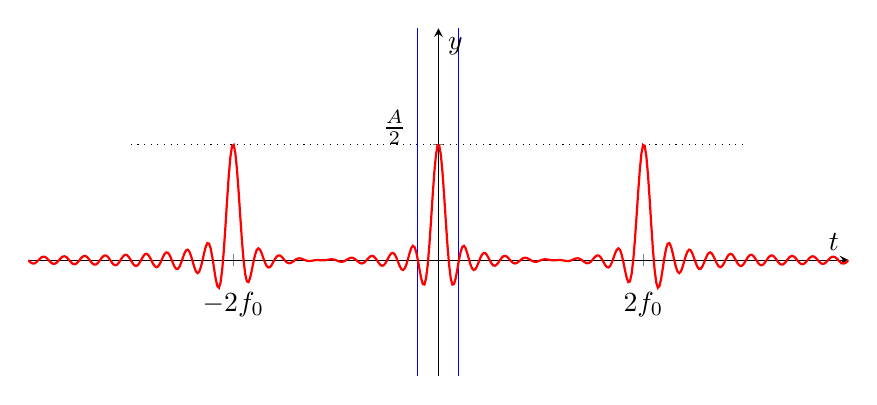
\begin{tikzpicture}
                        \begin{axis}[
                            domain=-40:40,
                            samples=200,
                            axis lines=middle,
                            xlabel=$t$,
                            ylabel=$y$,
                            ytick = {0.5},
                            yticklabels = {$\frac{A}{2}$},
                            yticklabel style = {yshift=6pt,xshift=-6pt},
                            xtick = {-20,20},
                            xticklabels = {$-2f_0$,$2f_0$},
                            xticklabel style = {yshift=-6pt}, 
                            ymin=-0.5,
                            ymax=1,
                            width=12cm,
                            height=6cm
                        ]
                        \addplot [const plot, dotted,black] coordinates{(-30,0.5)(30,0.5)};
                        \addplot [const plot,blue] coordinates{(-2,-0.5)(-2,1)};
                        \addplot [const plot,blue] coordinates{(2,-0.5)(2,1)};
                        \addplot [red, thick, samples = 500] {(sin(deg((x)*pi))/(2*(x)*pi))+(sin(deg((x-20)*pi))/(2*(x-20)*pi))+(sin(deg((x+20)*pi))/(2*(x+20)*pi))};
                        \end{axis}
                    \end{tikzpicture}
                    \label{fig:demodulazione di una sinc}
                }
                \caption{Demodulazione di una $sinc$}
            \end{figure}
            Nel caso di piú segnali durante la demodulazione il segnale che voglio recuperare viene spostato in {\color{blue}BB}
            mentre gli altri segnali presenti sullo spettro vengono a loro volta modulati peró con un $f_0$ diverso rispetto al loro $f_0^\prime$:
            \begin{figure}[H]
                \centering
                \subfloat[Due $sinc$ modulate]{
                    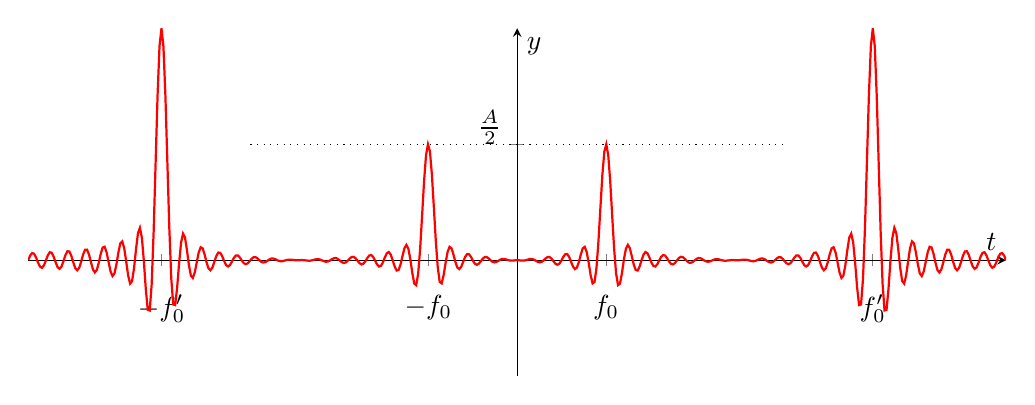
\begin{tikzpicture}
                        \begin{axis}[
                            domain=-55:55,
                            samples=200,
                            axis lines=middle,
                            xlabel=$t$,
                            ylabel=$y$,
                            ytick = {0.5},
                            yticklabels = {$\frac{A}{2}$},
                            yticklabel style = {yshift=6pt},
                            xtick = {-40,-10,10,40},
                            xticklabels = {$-f_0^\prime$,$-f_0$,$f_0$,$f_0^\prime$},
                            xticklabel style = {yshift=-7pt}, 
                            ymin=-0.5,
                            ymax=1,
                            width=14cm,
                            height=6cm
                        ]
                        \addplot [const plot, dotted,black] coordinates{(-30,0.5)(30,0.5)};
                        \addplot [red, thick, samples = 500] {(sin(deg((x-10)*pi))/(2*(x-10)*pi))+(sin(deg((x+10)*pi))/(2*(x+10)*pi))+(sin(deg((x-40)*pi))/((x-40)*pi))+(sin(deg((x+40)*pi))/((x+40)*pi))};
                        \end{axis}
                    \end{tikzpicture}
                    \label{fig:due sinc modulate}
                }
                \hfill
                \subfloat[Demodulazione delle $sinc$]{
                    \begin{tikzpicture}
                        \begin{axis}[
                            domain=-55:55,
                            samples=200,
                            axis lines=middle,
                            xlabel=$t$,
                            ylabel=$y$,
                            ytick = {0.5},
                            yticklabels = {$\frac{A}{2}$},
                            yticklabel style = {yshift=6pt,xshift=-6pt},
                            xtick = {-50,-40,-30,-20,20,30,40,50},
                            xticklabels = {$-f_0^\prime-f_0$,$-f_0^\prime$,$-f_0^\prime+f_0$,$-2f_0$,$2f_0$,$f_0^\prime-f_0$,$f_0^\prime$,$f_0^\prime+f_0$},
                            xticklabel style = {yshift=-6pt,font=\tiny}, 
                            ymin=-0.5,
                            ymax=1,
                            width=14cm,
                            height=6cm
                        ]
                        \addplot [const plot, dotted,black] coordinates{(-30,0.5)(30,0.5)};
                        \addplot [const plot,blue] coordinates{(-2,-0.5)(-2,1)};
                        \addplot [const plot,blue] coordinates{(2,-0.5)(2,1)};
                        \addplot [red, thick, samples = 800] {(sin(deg((x)*pi))/(2*(x)*pi))+(sin(deg((x-20)*pi))/(2*(x-20)*pi))+(sin(deg((x+20)*pi))/(2*(x+20)*pi))+(sin(deg((x-50)*pi))/(2*(x-50)*pi))+(sin(deg((x-30)*pi))/(2*(x-30)*pi))+(sin(deg((x+50)*pi))/(2*(x+50)*pi))+(sin(deg((x+30)*pi))/(2*(x+30)*pi))};
                        \end{axis}
                    \end{tikzpicture}
                    \label{fig:demodulazione di due sinc}
                }
                \caption{Demodulazione di due $sinc$}
            \end{figure}
            Potrei peró trovarmi in situazioni delle quali non posso recuperare il segnale
            \begin{figure}[H]
                \centering
                \subfloat[Due $sinc$ modulate]{
                    \begin{tikzpicture}
                        \begin{axis}[
                            domain=-55:55,
                            samples=200,
                            axis lines=middle,
                            xlabel=$t$,
                            ylabel=$y$,
                            ytick = {0.5},
                            yticklabels = {$\frac{A}{2}$},
                            yticklabel style = {yshift=6pt},
                            xtick = {-20,-18,18,20},
                            xticklabels = {$-f_0^\prime$,$-f_0$,$f_0$,$f_0^\prime$},
                            xticklabel style = {yshift=-7pt,font=\tiny}, 
                            ymin=-0.5,
                            ymax=1,
                            width=14cm,
                            height=6cm
                        ]
                        \addplot [const plot, dotted,black] coordinates{(-30,0.5)(30,0.5)};
                        \addplot [red, thick, samples = 500] {(sin(deg((x-18)*pi))/(2*(x-18)*pi))+(sin(deg((x+18)*pi))/(2*(x+18)*pi))+(sin(deg((x-20)*pi))/((x-20)*pi))+(sin(deg((x+20)*pi))/((x+20)*pi))};
                        \end{axis}
                    \end{tikzpicture}
                    \label{fig:sinc non recuperabile}
                }
                \hfill
                \subfloat[Demodulazione delle $sinc$]{
                    \begin{tikzpicture}
                        \begin{axis}[
                            domain=-55:55,
                            samples=200,
                            axis lines=middle,
                            xlabel=$t$,
                            ylabel=$y$,
                            ytick = {0.5},
                            yticklabels = {$\frac{A}{2}$},
                            yticklabel style = {yshift=6pt,xshift=-6pt},
                            xtick = {-38,-36,-2,2,36,38},
                            xticklabels = {$-f_0^\prime-f_0$,,$-2f_0$$-f_0^\prime+f_0$,$f_0^\prime-f_0$,$2f_0$,$f_0^\prime+f_0$},
                            xticklabel style = {yshift=-6pt,font=\tiny,rotate=90}, 
                            ymin=-0.5,
                            ymax=1,
                            width=14cm,
                            height=6cm
                        ]
                        \addplot [const plot, dotted,black] coordinates{(-30,0.5)(30,0.5)};
                        \addplot [const plot,blue] coordinates{(-2,-0.5)(-2,1)};
                        \addplot [const plot,blue] coordinates{(2,-0.5)(2,1)};
                        \addplot [red, thick, samples = 800] {(sin(deg((x)*pi))/(2*(x)*pi))+(sin(deg((x-36)*pi))/(2*(x-36)*pi))+(sin(deg((x+36)*pi))/(2*(x+36)*pi))+(sin(deg((x-38)*pi))/(2*(x-38)*pi))+(sin(deg((x-2)*pi))/(2*(x-2)*pi))+(sin(deg((x+38)*pi))/(2*(x+38)*pi))+(sin(deg((x+2)*pi))/(2*(x+2)*pi))};
                        \end{axis}
                    \end{tikzpicture}
                    \label{fig:demodulazione sinc non recuperabile}
                }
                \caption{Demodulazione di due $sinc$ non recuperabili}
            \end{figure}
            Come possiamo vedere nella regione della {\color{blue}BB}, il segnale é molto sporco, magari puó essere confuso con un 
            $\cos$ e non una sinc. inoltre ora qui ho usato numeri interi per fare il $plot$ quindi non si accavallano cosí male 
            ma si accavallano solo in $\frac{1}{T}$ se usassi altri valori sarebbe ancora piú sporco il segnale.\\
            
            Adesso proviamo a calcolare quanti segnali possiamo trasmettere in una banda:\\
            
            \indent{
                Ho un segnale rettangolare che dura $5$ minuti e una banda di $20MHz = 20\dotproduct 10^6Hz$\\
                \begin{gather}
                        f_{segnale}=\frac{1}{5\dotproduct60} =\frac{1}{300}Hz  \nonumber \\
                        n^{\circ}\ di\ segnali = \frac{20\dotproduct 10^6}{f_{segnale}} = 20\dotproduct 10^6 \dotproduct 300 = 6\dotproduct 10^9 \nonumber
                \end{gather}
            }
            \begin{figure}[H]
                \centering
                \begin{tikzpicture}
                    \begin{axis}[
                        domain=-4:4,
                        samples=200,
                        axis lines=middle,
                        xlabel=$x$,
                        ymin=-0.2,
                        ymax=0.2,
                        xtick={-2,0,2},
                        xticklabels={$f_{lower\ bound}$,$0$,$f_{upper\ bound}$},
                        ytick={},
                        width=10cm,
                        height=4cm
                    ]
                    \addplot [const plot,blue, thick] coordinates{(-2,0)(2,0)};
                    \end{axis}
                \end{tikzpicture}
                \caption{Spettro per la trasmissione}
                \label{fig:banda esercizio segnali}
            \end{figure}    
            \subsubsection{Funzionamento di un Radar}
                \begin{figure}[H]
                    \centering
                    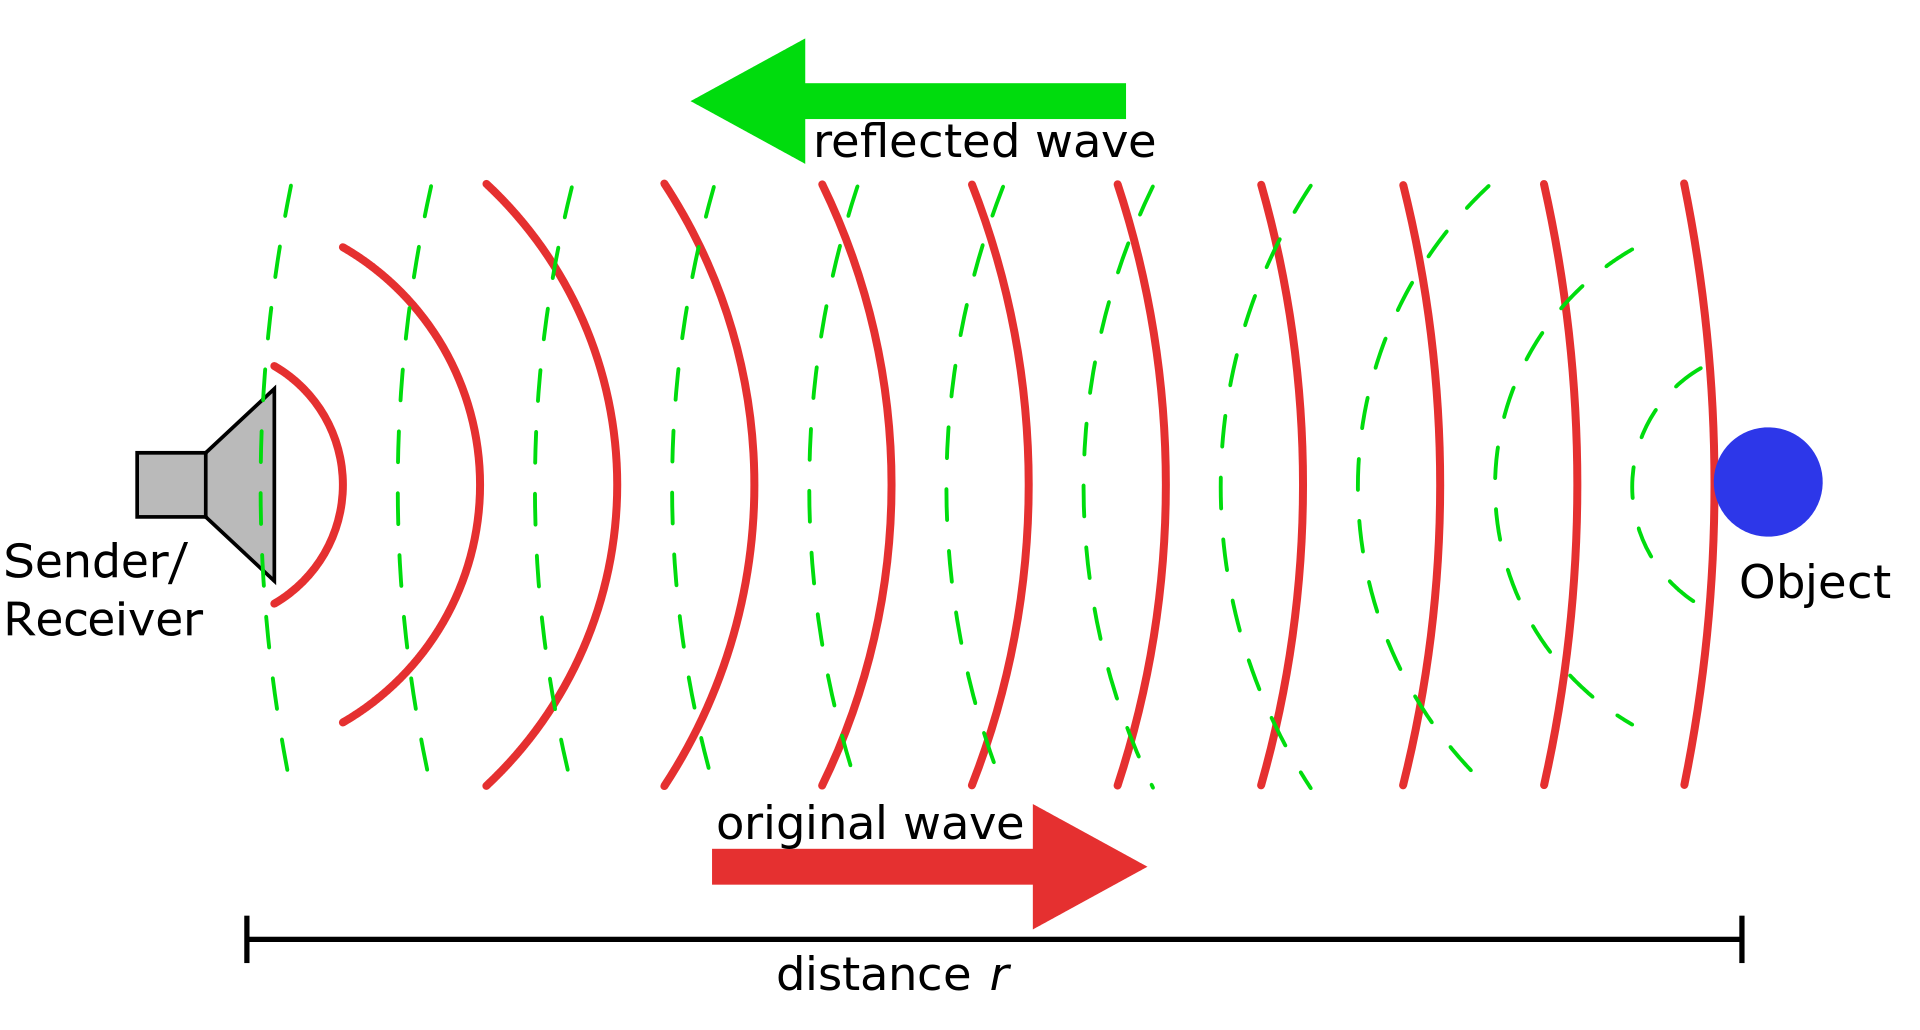
\includegraphics[width=8cm]{media/radar.png}
                    \caption{Spettro per la trasmissione}
                    \label{fig:esempio radar}
                \end{figure}    
                La sorgente emette un'{\color{red}onda} continua e passivamente capta per le {\color{green}onde} riflesse dagli oggetti.
                Il calcolo della distanza si basa sulla capacitá dei materiali di riflettere le onde, piú la frequenza dell'onda é alta 
                piú i materiali riescono a riflettere. L'emettitore, in presenza di ostacolo, riceve il segnale riflesso ({\em eco})
                e misura il ritardo dell'{\em eco} rispetto al segnale originale per poi calcolarne la distanza. Prendiamo un emettitore di onde 
                rettangolari.
                \begin{figure}[H]
                    \centering
                    \begin{tikzpicture}
                        \begin{axis}[
                            domain=-0:10,
                            samples=200,
                            axis lines=middle,
                            xlabel=$t$,
                            ylabel=$y$,
                            ymin=-0.2,
                            ymax=3,
                            xtick={0,2,4,6},
                            xticklabels={$0$,$T$,$\tau$,$\tau+T$},
                            ytick={},
                            width=10cm,
                            height=4cm
                        ]
                        \addplot [const plot,red, thick] coordinates{(0,0)(0,2)};
                        \addplot [const plot,red, thick] coordinates{(0,2)(2,2)};
                        \addplot [const plot,red, thick] coordinates{(2,2)(2,0)};

                        \addplot [const plot,green, thick] coordinates{(4,0)(4,1)};
                        \addplot [const plot,green, thick] coordinates{(4,1)(6,1)};
                        \addplot [const plot,green, thick] coordinates{(6,1)(6,0)};
                        \end{axis}
                    \end{tikzpicture}
                    \caption{Spettro per la trasmissione}
                    \label{fig:radar rettangolare}
                \end{figure}    
                Indichiamo con $\tau$ il ritardo di ricezione dell'{\em eco} e la distanza che sempara il radar dall'oggetto $d$:
                \[
                    d=\frac{c\tau}{2}
                \]
                Compare un fattore $\frac{1}{2}$ dovuto al segnale che percorre due volte la distanza tra l'emettitore e l'oggetto.
                Possiamo notare che l'{\em eco} ha ampiezza minore poiché dell'energia é stata assorbita dal materiale o una porzione del segnale
                originale ha oltrepassato il materiale stesso.
                
                Analizziamo in frequenza cosa succede. 
                
                Volgiamo realizzare un radar a onda rettagolare che rileva a un massimo di $15$ metri di distanza e a un minimo di $1,5$ metri.
                Possiamo calcolare i valori di ritardo massimo e minimo:
                \begin{gather}
                    \tau_{min} =\frac{2\dotproduct 15}{3\dotproduct 10^8} =10^{-7} = 0.1\mu s  \nonumber\\
                    \tau_{max} =\frac{2\dotproduct 1.5}{3\dotproduct 10^8} =10^{-7} = 10 ns\nonumber
                \end{gather}  
                Il radar funziona finché $T<<\tau_{min}$, se avessi un $\tau_{min}>T$ non potrei distinguere il segnale inviato da quello ricevuto.  
                \begin{figure}[H]
                    \centering
                    \begin{tikzpicture}
                        \begin{axis}[
                            domain=-0:10,
                            samples=200,
                            axis lines=middle,
                            xlabel=$t$,
                            ylabel=$y$,
                            ymin=-0.2,
                            ymax=3,
                            xtick={0,2,2.4,4,6},
                            xticklabels={$0$,$T$,$\tau_{min}$,$\tau_{max}$,$\tau+T$},
                            ytick={},
                            width=10cm,
                            height=4cm
                        ]
                        \addplot [const plot,red, thick] coordinates{(0,0)(0,2)};
                        \addplot [const plot,red, thick] coordinates{(0,2)(2,2)};
                        \addplot [const plot,red, thick] coordinates{(2,2)(2,0)};

                        \addplot [const plot,green, thick] coordinates{(4,0)(4,1)};
                        \addplot [const plot,green, thick] coordinates{(4,1)(6,1)};
                        \addplot [const plot,green, thick] coordinates{(6,1)(6,0)};
                        \end{axis}
                    \end{tikzpicture}
                    \caption{Limiti di ritardo del radar}
                    \label{fig:radar rettangolare limiti}
                \end{figure}    
                
                Nel nostro caso potremmo scegliere un $T\backsimeq 1ns \backsimeq 10^{-9}$ per rispettare i limiti imposti dall'esercizio.
                Ma analizzando l'intervallo frequenziale della $TCF$ della funzione rettangolo, una $sinc(x)$, il nostro segnale ha componenti
                frequenziali significative nell'ordine dei GHz, $\frac{1}{T}= \frac{1}{10^{-9}} = 1GHz$. I segnali nell'ordine dei GHz oltrepassano con facilitá
                gli ostacoli, basti vedere le bande di funzionamento dei cellulari e il Wi-Fi. Si utilizzano segnali con l'ordine di cetinaia se non igliaia di Hz, 
                possiamo vedere come la lunghezza d'onda del segnale giochi un ruolo fondamentale:
                
                \begin{gather}
                        \lambda_0 = \frac{c}{f_0} \nonumber \\
                        \lambda_0 = \begin{cases}
                            f_0 = 3GHz \rightarrow \lambda_0 = 0.1m \nonumber \\
                            f_0 = 30GHz \rightarrow \lambda_0 = 0.01m \nonumber \\
                            f_0 = 300GHz \rightarrow \lambda_0 = 0.001m \nonumber \\
                            f_0 = 3000GHz \rightarrow \lambda_0 = 0.0001m \nonumber 
                        \end{cases}\nonumber
                \end{gather}

            come funzionano il lidarr e il sonarr? come hanno fatto a rilevare i movimenti con il wifi?
    \subsection{Delta di Dirac}
        Si definisce Delta di Dirac $\delta_{(t)} = \derivative{}{t}U_{(t)}$ con $U_{(t)}$ funzione gradino.
        Piú correttamente si definisce Delta di Dirac la funzione che se integrata restituisce il gradino unitario:
        \[
            u_{(t)} = \int_{-\infty}^{\infty} \delta_{(t)} dt \rightarrow U_{(t)}
        \]

        \begin{figure}[H]
            \centering
            \begin{tikzpicture}
                \begin{axis}[
                    domain=-0:10,
                    samples=200,
                    axis lines=middle,
                    xlabel=$t$,
                    ylabel=$\delta_{(t)}$,
                    ymin=-0.2,
                    ymax=3,
                    xtick={0,2,2.4,4,6},
                    xticklabels={$0$,$T$,$\tau_{min}$,$\tau_{max}$,$\tau+T$},
                    ytick={2},
                    yticklabels={$1$},
                    width=10cm,
                    height=4cm
                ]
                \addplot [-stealth,purple,ultra thick] coordinates{(0,0)(0,2)};
                \end{axis}
            \end{tikzpicture}
            \caption{Delta di Dirac}
            \label{fig:Grafico Delta Di DIrac}
        \end{figure}    
        L'ampiezza della funzione é dovuta alla costante moltiplicativa, ma alla fin fine rimane sempre una funzione impulso.\\

        \textbf{boh amplia magari}
        
        \subsubsection{Propietá del Delta di Dirac}\label{Propietá del Delta di Dirac}
                \begin{itemize}
                    \item {
                        $\int_{-\infty}^{\infty} \delta_{(t)} dt = 1$
                    }\label{PD1}
                    \item {
                        Propietá Campionatrice:\\
                        $Ip:\ x_{(t)}\ continua\ in\ t_0$
                        \[
                            \int_{-\infty}^{\infty}x_{(t)}\delta_{(t-t_0)} dt = x_{(t_0)}  
                        \]
                        \begin{figure}[H]
                            \centering
                            \begin{tikzpicture}
                                \begin{axis}[
                                    domain=-0:6,
                                    samples=200,
                                    axis lines=middle,
                                    xlabel=$t$,
                                    ylabel=$x_{(t)}$,
                                    ymin=-0.2,
                                    ymax=5,
                                    xtick={2},
                                    xticklabels={$t_0$},
                                    ytick={3},
                                    yticklabels={$3$},
                                    width=10cm,
                                    height=8cm
                                ]
                                \addplot [-stealth,purple,ultra thick] coordinates{(2,0)(2,2.6)};
                                \addplot [blue,thick,samples = 300] {cos(deg(x))+3};
                                \end{axis}
                            \end{tikzpicture}
                            \caption{Propietá Campionatrice}
                            \label{fig:Grafico P. Campionatrice}
                        \end{figure} 
                    }\label{PD2}
                    \item {
                        Paritá: $\delta_{(t)} = \delta_{(-t)}$
                    }\label{PD3}
                    \item {
                        $x_{(t)}\delta_{(t-t_0)} dt = x_{(t_0)}\delta_{(t-t_0)}  $
                    }\label{PD4}
                    \item {
                        $x_{(t)} \otimes \delta_{(t)} = x_{(t)}$
                        Dimostrazione:
                        \[x_{(t)} \otimes \delta_{(t)} = \int_{-\infty}^{\infty}x_{(\tau)}\delta_{(t-\tau)} d\tau \Rightarrow^{\ref{PD3}} \int_{-\infty}^{\infty}x_{(\tau)}\delta_{(\tau-t)} d\tau = x_{(t)}\]
                    }\label{PD5}
                    \item {
                        $x_{(t)} \otimes \delta_{(t-t_0)} = x_{(t-t_0)}$
                        Dimostrazione:
                        \[x_{(t)} \otimes \delta_{(t-t_0)} = \int_{-\infty}^{\infty}x_{(\tau)}\delta_{(t-t_0-\tau)} d\tau \Rightarrow^{\ref{PD3}} \int_{-\infty}^{\infty}x_{(\tau)}\delta_{(\tau-(t-t_0))} d\tau = x_{(t-t_0)}\]
                    }\label{PD6}
                \end{itemize}
        \subsubsection{$TCF$ della Delta di Dirac}\label{TCF della Delta di Dirac}
                $x_{(t)} = A\delta_{(t)}$
                \[
                    TCF[x_{(t)}] = \int_{-\infty}^{\infty}\delta_{(t)}e^{-j2\pi ft} dt \Rightarrow^{\ref{PD2} t_0=0} \eval{e^{-j2\pi ft}}_{t=0} = A
                \]
                \begin{gather}
                        A\delta_{(t)} \leftrightharpoons^{TCF} A \nonumber \\
                        Per\ la\ dualita\ \ref{Dualita}: \nonumber \\
                        A \leftrightharpoons^{TCF} A\delta_{(-f)} = A\delta_{(f)}  \nonumber 
                \end{gather}
                Caso con ritardo:
                \begin{gather}
                    A\delta_{(t-t_0)} \leftrightharpoons^{TCF} Ae^{-j2\pi ft_0} \nonumber \\
                    Per\ la\ dualita\ \ref{Dualita}: \nonumber \\
                    Ae^{-j2\pi f_0t} \leftrightharpoons^{TCF} A\delta_{(-f-f_0)} {\color{red}\ oppure\ A\delta_{(f+f_0)?}} \nonumber 
                \end{gather}
    \section{Teoria Dei Codici}
    \subsection{Introduzione}
        Ci concentriamo adesso sul trattamento dell'informazione per poterla trasmettere.
        I messaggi che trasmettiamo possono essere codificati per vari motivi:
        \begin{itemize}
            \item {
                    Compressione:$\begin{cases}
                        \text{Lossy: con perdita dell'informazione} \nonumber\\
                        \text{Lossless: minima perdita dell'informazione} \nonumber
                    \end{cases}$\\
                    Comprimere l'informazione in elimenando ridondanza e salvando spazio di memoria e banda.
                    
                }
            \item {
                    Crittografia: per nascondere il messaggio ad utenti in ascolto sul canale che non siano il destinatario.
            }
            \item {
                    Rivelazione o correzione di errore: vieen aggiunta ridondanza ad hoc per aumentare l'affidabilitá del messaggio trasmesso. 
                    Si utilizzano \href{https://en.wikipedia.org/wiki/Checksum}{checksum} o \href{https://en.wikipedia.org/wiki/Reed-Solomon_error_correction}{Reed-Solomon(RS)}
            }
        \end{itemize}
        \paragraph{Capacitá del canale}\label{Capacita del canale}\index{Capacitá del canale}
            La capacitá del canale $C$ indica la massima quantitá d'informazione che puó essere trasmessain maniera affidabile su di un dato canale.
            La capacitá dipende dalla banda $B$ del canale e dal rapporto segnale rumore (signal-to-noise ratio,\href{https://en.wikipedia.org/wiki/Signal-to-noise_ratio}{$SNR$}):
            \[
                C = B\log(1 + SNR)  
            \] 
        \paragraph{Canale Gaussiano}\index{Canale Gaussiano}
            Il canale Gaussiano puó essere modellato come \href{https://en.wikipedia.org/wiki/Binary_symmetric_channel}{Binary Symmetric Channel (BSC)} con probabilitá di errore $p$. 
            Assumiamo gli errori tra loro indipendenti ($p_{(a,b)} = p_{(a)}\dotproduct p_{(b)}$):
        \begin{figure}[H]
            \centering
            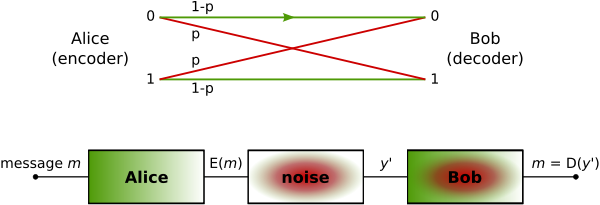
\includegraphics[width = 12cm]{media/600px-Binary_symmetric_channel_(en).svg.png}
            \label{BSC system}
            \caption{Sistema di trasmissione BSC}
        \end{figure}
        \begin{gather}
            E_{(x)}: \text{Funzione di codifica} \nonumber \\
            D_{(x)}: \text{Funzione di decodifica} \nonumber \\
            E_{(m)}: \text{Bit dell'informazione codificati} \nonumber \\
            y^\prime: E_{(m)}+ e \rightarrow \text{Informazioni con errore del canale} \nonumber \\
            m = D_{(y^\prime)}: \text{Informazione decodificata} \nonumber 
        \end{gather}
        Il canale é chiamato simmetrico perché ho la stessa probabilitá errore sulla trasmissione di uno dei due bit.
        Se $X$ é il bit inviato e Y quello ricevuto allora il canale é caratterizzato dalle probabilitá:
        \begin{align}
            P(Y=0|X=0) &= 1-p\nonumber \\
            P(Y=0|X=1) &= p\nonumber \\
            P(Y=1|X=0) &= p\nonumber \\
            P(Y=1|X=1) &= 1-p\nonumber 
        \end{align} 
        Assumiamo che $0\leq p \leq\frac{1}{2}$, se avessimo $p >\frac{1}{2}$ il ricevitore potrebbe scambiare l'informazione ricevuta
        (Quando riceve un $1$ lo interpreta come $0$ e viceversa) e ottenere un canale con probabilitá $1-p \leq\frac{1}{2}$. 
        
        Nel corso useremo delle simbologie diverse:
        \begin{figure}[H]
            \centering
            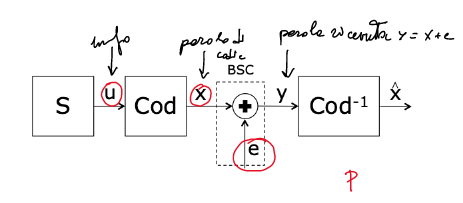
\includegraphics[width = 12cm]{media/BSC System.png}
            \label{BSC system moretti}
            \caption{Sistema di trasmissione BSC}
        \end{figure}
        \begin{gather}
            u: \text{Informazione} \nonumber \\
            x: \text{Parole di Codice} \nonumber \\
            e: \text{Errore del Canale} \nonumber \\
            y: x+e \rightarrow \text{Informazioni con errore del canale} \nonumber \\
            \overset{\wedge}{x}: \text{Informazione decodificata} \nonumber 
        \end{gather}
        \paragraph{Probabilitá di errore BSC}\label{Probabilita di errore BSC}\index{Probabilitá di errore BSC}
            La probabilitá, per una trasmissione BSC, di sbagliare $t$ bit in una parola di $n$ bit:
            \[
                p_{(t,n)} = \binom{n}{t} p^t (1-p)^{(n-t)}
            \]
            dove il coefficente binomiale:
            \[
                \binom{n}{t} = \frac{n!}{t!(n-t)!}
            \]
            indica tutte le possibili combinazioni di errori di $t$ bit su $n$ bit. 
        \paragraph{Tassonomia dei codici}
            \begin{itemize}
                \item {Codici lineari
                        \begin{itemize}
                            \item {
                                Codici a blocco
                                }
                            \item{
                                Codici convoluzionali
                            } 
                        \end{itemize}
                    }
                \item {
                    Definizione di un codice a blocco: 
                    \begin{figure}[H]
                        \centering 
                        \begin{tikzpicture}[
                            node distance=2cm,
                            >=latex
                            ]

                            \node [coordinate] (input) {};
                            \node [draw, rectangle,right of = input, minimum height=3em, minimum width=6em] (block) {$x_{(t)}$};
                            \node [coordinate, right of = block] (output) {};
                            
                            \draw[draw,->] (input) -- node[midway]{$/$} node[below]{$k$} (block);
                            \draw[->] (block) -- node[midway]{$/$} node[below]{$n$} (output);
                        \end{tikzpicture}    
                    \label{Def codice a blocco}
                    \end{figure}
                    \paragraph{Rate del Codice}:\index{Rate del Codice}
                        {
                            \[
                                R = \frac{k}{n}  
                            \]
                            La condizione é che $n>k$ senon fosse cosí avrei perdita d'informazione, da $k$ bit passo a $n$ aggiungendo
                            ridondanza e codificando i miei dati. Possiamo quindi stimare il valore tipico di $R$
                            \[
                                R = \frac{k}{n} <1  
                            \]
                        }
                }
                \item Rivelazione di errore:\index{Rivelazione di errore}{
                    Consiste nella capacità di scoprire la presenza di errori causati dal rumore o da altri fenomeni deterioranti 
                    durante una trasmissione di dati (es. tramite il \href{https://it.wikipedia.org/wiki/Bit_di_parit%C3%A0}{bit di paritá}).
                }
                \item {Correzione di errore:\index{Correzione di errore}{
                    Consiste invece nell'ulteriore abilità di ricostruire i dati originali, eliminando gli errori occorsi durante la trasmissione.
                    Vi sono due differenti schemi di base per la progettazione della codifica di canale e del protocollo per un sistema che corregge gli errori:
                    \begin{itemize}
                        \item {
                            ??\href{https://it.wikipedia.org/wiki/Automatic_repeat-request}{Automatic repeat-request} (ARQ): Il mittente invia i dati ed anche un codice a rilevazione d'errore, che sarà
                            utilizzato in ricezione per individuare gli eventuali errori, ed in tal caso chiedere la ritrasmissione dei dati
                            corrotti. In molti casi la richiesta è implicita; il destinatario invia un acknowledgement (ACK) di corretta 
                            ricezione dei dati, ed il mittente re-invia solo quei dati per i quali non ha ricevuto, entro un prefissato tempo 
                            limite (timeout), il corrispondente ACK.
                        }
                        \item{
                            ??\href{https://it.wikipedia.org/wiki/Forward_Error_Correction}{Forward Error Correction} (FEC): Il mittente codifica i dati con un codice a correzione d'errore 
                            (error correction code, ECC) ed invia il messaggio codificato. Il destinatario non invia mai alcun 
                            messaggio verso il mittente; esso decodifica ciò che riceve nella maniera più simile possibile a quella di un 
                            certo insieme prefissato di parole accettabili. Tali codici sono realizzati in modo tale che dovrebbe occorrere 
                            una quantità "irragionevole" di errori nei dati, affinché il destinatario decodifichi erroneamente, ottenendo 
                            finalmente dei dati diversi da quelli effettivamente inviatigli.
                        } 
                    \end{itemize}
                    In generale un codice a blocco che ha rate $\frac{k}{n}$ mappa $k$ bit su $n$ bit usando $2^k$ parole di codice di dimensione n
                }}
            \end{itemize}

        \subsubsection{Esempio codici a blocco: codici a ripetizione}
            É un esempio di codice a correzione d'errore: il funzionamento si basa sulal ripetizione dell'informazione piú volte. Il destinatario
            si accorge di un errore di trasmissione poiché il flusso di dati ricevuto non è la ripetizione di un singolo messaggio e, inoltre, 
            il destinatario può recuperare il messaggio originale guardando il messaggio ricevuto nel flusso di dati che si verifica più spesso.

            Nel caso di un codice binario di ripetizione, esistono due parole in codice - tutte uno e tutti zeri - che hanno una lunghezza n. 
            Pertanto, la distanza minima di Hamming (\ref{Distanza di Hamming}) del codice è uguale alla sua lunghezza. Ciò conferisce al codice 
            di ripetizione, con $R = \frac{1}{n}$,una capacità di rivelazione di errori pari a $n-1$ e correzione degli errori (cioè correggerà fino agli errori in qualsiasi parola del codice) di $\frac{n-1}{2}$ per n dispari(\ref{Probabilita di errore BSC}).\\
            Esempio:\\
            \indent{$R = \frac{1}{3} \rightarrow$ ha solo 2 parole di codice:}
            \begin{align}
                u=0 \rightarrow x = [000]\nonumber \\
                u=1 \rightarrow x = [111]\nonumber
            \end{align} 
            Il ricevitore effettua una decodifica a maggioranza: decide per il bit che comprare piú volte della parola ricevuta.
            \begin{align}
                y = [000] \rightarrow \overset{\wedge}{x} = [000] \rightarrow \overset{\wedge}{u} = 0 \nonumber \\
                y = [010] \rightarrow \overset{\wedge}{x} = [000] \rightarrow \overset{\wedge}{u} = 0 \nonumber \\
                y = [101] \rightarrow \overset{\wedge}{x} = [111] \rightarrow \overset{\wedge}{u} = 1 \nonumber
            \end{align}
            \paragraph{Evento errore:} l'evento errore per un codice a correzione di errore consiste nel non essere in grado di correggere
            tutti gli errori introdotti dal canale. Se la probabilitá di errore sul bit $p_{e,b}$ é piccola, la probabilitá di errore 
            $p_{e,W}$ per il codice puó essere approssimata dal primo evento che determina la ricezione errata (nel caso dei codici a ripetizione a $R = \frac{1}{3}$ 
            si verifichino $2$ errori).
            \begin{itemize}
                \item {$R = \frac{1}{3}$
                    \begin{itemize}
                        \item {
                            Se $p_{e,b} = 0.1 \Rightarrow p_{e,W} \approx 2.7\dotproduct 10^{-2} $ 
                        }
                        \item {
                            Se $p_{e,b} = 0.01 \Rightarrow p_{e,W} \approx 2.97\dotproduct 10^{-4} $ 
                        }
                    \end{itemize}
                }
                \item {$R = \frac{1}{5}$
                    \begin{itemize}
                        \item {
                            Se $p_{e,b} = 0.1 \Rightarrow p_{e,W} \approx 8.1\dotproduct 10^{-3} $ 
                        }
                        \item {
                            Se $p_{e,b} = 0.01 \Rightarrow p_{e,W} \approx 9.8\dotproduct 10^{-6} $, Sviluppiamo i calcoli come esempio: 
                            \[
                                P_r \{\text{codice }R=\frac{1}{5}\text{ non riesce a correggere gli errori introdotti dal canale}\}:
                            \]
                            \begin{align}
                                P_r &= \sum_{t=3}^{5} \binom{5}{t}p^t (1-p)^{5-t},\hspace{0.2cm} p=10^{-2} \nonumber \\
                                P_r &\{\text{3 errori su 5}\}= \binom{5}{3}p^3 (1-p)^{5-3} = 10\dotproduct 10^{-6} (0.99)^2 = 9.8\dotproduct 10^{-6} \nonumber \\
                                P_r &\{\text{3 errori su 5}\}= \binom{5}{4}p^4 (1-p)^{5-4} = 5\dotproduct 10^{-8} (0.99) = 5\dotproduct 10^{-8}\nonumber \\
                                P_r &\{\text{3 errori su 5}\}= \binom{5}{5}p^5 (1-p)^{5-5} = 1\dotproduct 10^{-10} = 10^{-10}\nonumber 
                            \end{align}
                        }
                    \end{itemize}
                }
            \end{itemize}

        \subsubsection{Esempio codici a blocco: codici a controllo di paritá}
        Il bit di parità è un codice di controllo d'errore, utilizzato nei calcolatori per prevenire errori nella trasmissione o nella memorizzazione dei dati. 
        Tale codice prevede l'aggiunta di un bit ridondante ai dati, calcolato a seconda che il numero di bit che valgono 1 sia pari o dispari. Ne esistono
        quindi 2 varitá: bit di paritá pari e bit di paritá dispari. Quando si usa il bit di paritá pari si aggiunge un bit con valore $1$ se nella parola inviata
        il numero di occorrenze di "$1$" é dispari(portando il numero di occorrenze di "$1$" a una quantitá pari).Quando si usa il bit di paritá dispari si
        aggiunge un bit con valore $1$ se nella parola inviata il numero di occorrenze di "$1$" é pari (portando il numero di occorrenze di "$1$" a una quantitá dispari).

        \noindent Il codice ha $R = \frac{k}{(k+1)}$: $k$ bit informativi piú il bit di paritá.
        
        \paragraph{Rilevazione dell'errore:}La rilevazione d'errore deriva dalla discordanza del numero di occorrenze di "$1$", eseguendo lo XOR bit a bit, nel caso del bit di paritá pari, se il risultato
        é $0$ non sono avvenuti errori, viceversa se ho un risultato uguale a $1$ posso dire che cé stato uno o una quantitá dispari di errori nella trasmissione, questo lo rende
        solo un codice a rilevazione d'errore e non un codice a correzione d'errore.
        
        Esempio:Trasmetto parole di $11bit$ con rate $R_b = 10Mb/s$ e probabilitá di errore sul bit trasmesso $p_{e,b} = 10^{-8}$:
        \begin{itemize}
            \item {
                Senza controllo di paritá é sufficiente che sia sbagliato anche un solo bit per sbagliare tutta la parola:
                \[
                    p_{e,W} = \sum_{j=1}^{11} \binom{11}{j}p_{e,b}^j (1-p_{e,b})^{11-j} = 11 p_{e,b} (1-p_{e,b})^{10} \simeq 11p_{e,b}
                \]
                ed il rate di parole sbagliate al secondo é:
                \[
                    R_{e,W} = \frac{R_b}{11}\dotproduct p_{e,W} \simeq \frac{10^7}{11}\dotproduct 11p_{e,b} = 0.1_\frac{w}{s}
                \]
            }
            \item {
                Aggiungendo un bit di paritá, la parola diventa di 12 bit e sbaglio quando faccio almeno 2 errori, il singolo errore
                viene corretto chiedendo nuovamente la trasmissione del dato:
                \[
                    p_{e,W} = \sum_{j=2}^{12} \binom{12}{j}p_{e,b}^j (1-p_{e,b})^{12-j} = 66 p_{e,b}^2 (1-p_{e,b})^{10} \simeq 66p_{e,b}^2
                \]
                ed il rate (frequenza) di parole sbagliate al secondo é:
                \[
                    R_{e,W} = \frac{R_b}{12}\dotproduct p_{e,W} \simeq \frac{10^7}{12}\dotproduct 66p_{e,b}^2 = 5.5\dotproduct 10^{-9} \frac{w}{s}
                \]
                possiamo anche calcolare il periodo $T_{e,W} = \frac{1}{R_{e,W}} =  1.82\dotproduct 10^{8} s$ che é una parola ogni sei anni circa.  
            }
        \end{itemize}
        \subsubsection{Esempio codici a blocco: codice ISBN}
            Il codice International Standard Book Number (ISBN) é un codice a controllo di paritá per un alfabeto di simboli nonbinari. 
            Ad ogni libro é assegnata una parola di codice di lunghezza $n=10$ cifre in base decimale. Le prime 9 cifre identificano il libro, 
            la decima é quella di controllo di paritá cosí calcolata:
            \begin{enumerate}
                \item {
                    Si calcola la grandezza $z = mod(S,11)$ con
                    \[
                        S = \sum_{j=1}^{9} (11-j)x_{(j)}
                    \]
                }
                \item {
                    La cifra di controllo di aritá é il complemento a 11 di $z$:
                    \[
                        x_{(10)} = mod(11-z,11)  
                    \]
                    E solo per la cifra di controllo di paritá se $x_{(10)} = 10$ si sostituisce con 
                    $x_{(10)} = X$
                }
            \end{enumerate}
            Quando un dispositivo legge il codice lo verifica come segue:
            \begin{enumerate}
                \item {
                    Moltiplica ogni cifra per il peso della posizione della stessa cifra e calcola $mod(S^\prime,11)$ con
                    \[
                        S^\prime = \sum_{j=1}^{10} (11-j)y_{(j)}
                    \]
                }
                \item {
                    Assumendo che non ci siano errori su $x_{(10)} = |11-z|_{11}$, si ha:
                    \begin{align}
                        mod(S^\prime,11) &= mod \left( \sum_{j=1}^{9} (11-j)y_{(j)} + mod(11-z,11),11\right) \nonumber \\
                                         &= mod \left( \sum_{j=1}^{9} (11-j)y_{(j)} + \left(11-\sum_{j=1}^{9} (11-j)x_{(j)}\right),11\right)\nonumber \\
                                         &= mod \left(\sum_{j=1}^{9} (11-j)(y_{(j)}-x_{(j)}),11\right)
                    \end{align}
                }
            \end{enumerate}
            Se non ci sono errori si ha $y=x$ e quindi il $mod(S^\prime,11) = 0$
            \paragraph{Rivalazione degli errori:} Il codice é in grado di rivelare tutti i singoli errori:
            sia $e_{(k)}$ l'errore in posizione $k$,$y_{(k)} = x_{(k)}+ e_{(k)}$:
            \[
                mod(S^\prime,11) = mod((y_{(k)}-x_{(k)})(11-k),11)+mod(e_{(k)}(11-k),11) \neq 0
            \]
            Il codice é in grado di rivelare tutti i casi in cui ci sia uno scambio di 2 cifre del codice. Siano 
            $k_1$ e $k_2$ le 2 posizioni scambiate:
            \begin{align}
                mod(S^\prime,11) &= mod \left((y_{(k_1)}-x_{(k_1)})(11-k_1)+(y_{(k_2)}-x_{(k_2)})(11-k_2),11\right) \nonumber \\
                                 &= mod \left((x_{(k_2)}-x_{(k_1)})(11-k_1)+(x_{(k_1)}-x_{(k_2)})(11-k_2),11\right)\nonumber \\
                                 &= mod \left((x_{(k_2)}-x_{(k_1)})(k_2-k_1),11\right) \neq 0 \nonumber
            \end{align}
            Esempi:
            \begin{itemize}
                \item {Senza errore:
                    \begin{align}
                        ISBN & = 01-333-5485-7 \nonumber \\
                        \left| S^\prime \right|_{11} &= 0\dotproduct 10 +1\dotproduct 9+3\dotproduct 8+3\dotproduct 7+3\dotproduct 6+5\dotproduct 5+4\dotproduct 4+8\dotproduct 3+5\dotproduct 2+7\dotproduct 1\nonumber \\
                        \left| S^\prime \right|_{11} &= \left| 154 \right|_{11} = 0 \nonumber 
                    \end{align}
                    Il codice é corretto 
                }
                \item {Con errore: Scambio le cifre
                    \begin{align}
                        ISBN & = 01-333-5458-7 \nonumber \\
                        \left| S^\prime \right|_{11} &= 0\dotproduct 10 +1\dotproduct 9+3\dotproduct 8+3\dotproduct 7+3\dotproduct 6+5\dotproduct 5+4\dotproduct 4+{\color{red}5\dotproduct 3}+{\color{red}8\dotproduct 2}+7\dotproduct 1\nonumber \\
                        \left| S^\prime \right|_{11} &= \left| 151 \right|_{11} = 8 \neq 0 \nonumber 
                    \end{align}
                    Il codice non é corretto 
                }
            \end{itemize}
        \subsection{Codici a blocco}
        \subsubsection{Introduzione ai codici lineari}
            \paragraph{Campo:} un campo é una struttura composta da un insieme non vuoto $F$ e da due operazioni binarie interne: $\forall \alpha,\beta,\gamma \in F$:
                \begin{itemize}
                    \item {
                        Somma ($XOR$):
                        \begin{itemize}
                            \item {
                                \[
                                    \alpha + \beta = \theta, \theta \in F  
                                \]
                            }
                            \item {Associativa:
                                \[
                                    (\alpha + \beta) + \gamma = \alpha +( \beta + \gamma)
                                \]
                            }
                            \item {Commutativa:
                                \[
                                    \alpha + \beta = \beta + \alpha
                                \]
                            }
                            \item {Elemento Neutro:
                                \[
                                    0\in F,\alpha + 0 = \alpha,\alpha-\alpha = 0
                                \]
                            }
                        \end{itemize}
                    }
                    \item {
                        Prodotto ($AND$):   
                        \begin{itemize}
                            \item {
                                \[
                                    \alpha \dotproduct \beta = \theta, \theta \in F  
                                \]
                            }
                            \item {Associativa:
                                \[
                                    (\alpha \dotproduct \beta) \dotproduct \gamma = \alpha \dotproduct( \beta \dotproduct \gamma)
                                \]
                            }
                            \item {Commutativa:
                                \[
                                    \alpha \dotproduct \beta = \beta \dotproduct \alpha
                                \]
                            }
                            \item {Distributiva:
                                \[
                                    (\alpha + \beta) \dotproduct \gamma = \alpha \dotproduct \gamma + \beta \dotproduct \gamma
                                \]
                            }
                            \item {Elemento Neutro:
                                \[
                                    1\in F,\alpha \dotproduct 1 = \alpha,\forall \alpha \neq 0\rightarrow \alpha\dotproduct\alpha^{-1} = 0
                                \]
                            }
                        \end{itemize}
                    }
                \end{itemize}
        \subsubsection{Campi di Galois}
            Un campo finito, detto anche campo di Galois, é un campo con un numero finito $q$ di elementi. Il numero di elementi di definisce la categoria del
            campo: $GF(2)$ é il campo definito su $\{0,1\}$ con somma modulo 2 ($XOR$) e prodotto modulo 2 ($AND$). Definito lo spazio $GF(2)$ si puó costruire
             lo spazio vettoriale $\mathcal{V}_n=GF(2)^2$, lo spazio di tutti i possibili $2^n$ vettori di $n$ cifre binarie su cui valgono le operazioni definite per 
             $GF(2)$.

        \subsubsection{Codici a blocco lineari su $GF(2)$}
            Sia $u = [u_1, \dots, u_k]$ una generica parola di $k$ cifre binarie. Il codice a blocco lineare $\mathcal{C}(k,n)\subset \mathcal{V}_n$ é l'insieme delle
            $2^k$ parole $x = [x_1, \dots, x_n]$ di $n$ cifre binarie ottenute con la trasformazione lineare:
            \[
                x = uG  
            \]
            Dove $G$ é la matrice generatrice del codice e ha dimensione $k \times n$ di cifre binarie con $n>k$ poiché al massimo
            aggiungo informazioni per la trasmissione, per la correzione o rivelazione d'errore.
            
            Siano $g_i, i = [1, \dots, k]$, le righe di $G$, $x$ é la combinazione lineare delle righe $g_i$:
            \[
                x = \sum_{i=1}^{k}u_ig_i  
            \]
            Per avere $2^k$ parole di codice distinte  é necessario che $G$ abbia rango $k$: le righe di $G$ devono essere linearmente indipendenti e costituiscono 
            una $base$ per il sottospazio vettoriale $\mathcal{C} \subset \mathcal{V}_n$.  

        \subsubsection{Propietá dei codici a blocco lineari}
            Le propietá derivano maggiormente dalla pripietá di linearit;a dei codici:
            \begin{itemize}
                \item {Ogni parola di codice é una combinazione lineare di righe della matrice generatrice.}
                \item {Il codice a blocchi é costituito da tutte le possibili combinazioni delle righe della matrice generatrice.}
                \item {La somma di due parle di codice é ancora una parola di codice.}
                \item {La $n-upla$ di tutti zeri é sempre una parola di codice.}
                \item {Se $x$ é una parola di codice, anche $-x$ é una parol di codice.}
            \end{itemize}

        \subsubsection{Distanza di Hamming}\label{Distanza di Hamming}\index{Distanza di Hamming}
            La distanza di Hamming tra due vettori, o stringhe, $d(x_1,x_2)$ di $n$ elementi é il nuemro di posizioni in cui le due parole
            sono diverse tra loro. Esempi:
            \begin{itemize}
                \item {
                    La distanza di Hamming tra 10{\color{red}1}1{\color{red}1}01 e 10{\color{red}0}1{\color{red}0}01 è 2.
                }
                \item {
                    La distanza di Hamming tra 2{\color{red}14}3{\color{red}8}96 e 2{\color{red}23}3{\color{red}7}96 è 3.
                }
            \end{itemize}
            \paragraph{Peso di Hamming:}\label{Peso di Hamming}\index{Peso di Hamming} Il peso di Hamming,$w(x)$, di una stringa i lunghezza $n$ é la sua distanza di Hamming dal vettore di $n$ zeri,
            $x_0\in \mathcal{V}_n$ é:
            \[
                w(x_0) = d(x_0,0_n)
            \]
            \paragraph{Distanza minima:}\label{Distanza minima}\index{Distanza minima}La distanza minima di un codice $\mathcal{C}$ é la minima distanza di Hamming calcolata fra tutte le possibili parole che appartengono a $\mathcal{C}$.
            \[
                d_{min} (\mathcal{C})= \underset{x_1,x_2 \in \mathcal{C}}{min}d(x_1,x_2)  
            \]
            Per i codici lineari vale che ciascuna parola di codice ha lo stesso insieme di distanze dalle altre parole di codice.
            La distanza minima di un codice si puó calcolare a partire da qualsiasi parola di codice. 
            La distanza di Hamming é una metrica:
            \begin{itemize}
                \item {}
                \item {}
                \item {}
                \item {}
            \end{itemize}
        \subsubsection{Codici a blocco in forma sistematica}
            Quando il codice é in forma sistematica la matrice generatrice del codice ha la seguente forma:
            \begin{gather}
                G = [I_k,P]\nonumber \\
                G\in k\times n,\ I\in k\times k,\ P\in k\times (n-k)\nonumber
            \end{gather}
            dove la matrice $P$ é la matrice di paritá, il suo contenuto dipende da quale algoritmo di paritá viene scelto.
            \begin{figure}[H]
                \centering 
                \begin{tikzpicture}[
                    node distance=2cm,
                    >=latex
                    ]

                    \node [coordinate] (input) {};
                    \node [draw, rectangle,right of = input, minimum height=3em, minimum width=6em] (block) {Coder};
                    \node [coordinate, right of = block] (output) {};
                    
                    \draw[draw,->] (input) -- node[midway]{$/$} node[below]{$k$} (block);
                    \draw[->] (block) -- node[midway]{$/$} node[below]{$n$} (output);
                \end{tikzpicture}    
            \label{Def codice forma sistematica}
            \end{figure}
            \begin{figure}[H]
                \centering 
                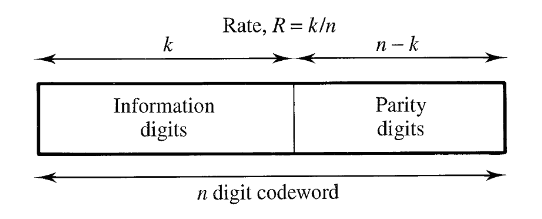
\includegraphics[width = 8cm]{media/forma sistematica.png}
            \label{matrice forma sistematica}
            \end{figure}
            \paragraph{Esempio Codice a ripetizione:}
            $R = \frac{1}{3},\ k=1,\ n=3$
            \begin{table}[H]
                \centering
                \begin{tabular}{|c|c|}
                \hline
                Bit i  ingresso & Parola codificata \\ \hline
                0               & {[}000{]}         \\ \hline
                1               & {[}111{]}         \\ \hline
                \end{tabular}
            \end{table}
            La matrice generatirce del codice é $G = [111]$, e la distanza minima $d_{min} = 3$\\

            \paragraph{Esempio Codice a controllo di paritá:}
            $R = \frac{7}{8},\ k=7,\ n=8$, ogni 7 bit ne aggiunge uno di controllo di paritá, 1 se il numero di "1" é diapari,
            0 se il numero di "1" é diapari.


            \noindent La matrice generatirce del codice:
            \[
                G = [I_7,1_7]
            \]
            \noindent La distanza minima é $d_{min} = 2$, se cambio uno dei 7 bit della parola
            cambio automaticamente il bit di paritá, quindi cambiare 1 bit in realtá ne cambia 2.\\

            \noindent Il prodotto $u\dotproduct 1_7 = \sum_{i=1}^{7}u_i$, puó essere scritto come una soma modulo 2, vale 0 se il numero di 
            occorrenze di "1" é pari e 1 altrimenti. Non facciamo altro che calcolare il bit di paritá della parola $u$.
            
            \paragraph{Definizione:} Due codici lineari $\mathcal{C}_1(k,n)$ e $\mathcal{C}_2(k,n)$ in $GF(2)$ sono equivalenti se uno é ottenuto dall'altro
            attraverso una permutazione delle posizioni del codice.

            \paragraph{Teorema:} Due matrici generatrici $G_1$ e $G_1$ in $GF(2)$ generano due codici equivalenti se una puó essere ottenuta dall'altra
            da una sequenza di operazioni come:
            \begin{itemize}
                \item Permutazione delle righe.
                \item Combinazione lineare delle righe.
                \item Permutazione delle colonne.
            \end{itemize}
            
            \paragraph{Teorema:} Qualsiasi codice lineare a blocchi é equivalente ad un codice in forma sistematica.

            \paragraph{Propietá degli spazi:}
            \begin{itemize}
                \item {
                    Dato il sottospazio $\mathcal{C} \subset \mathcal{V}_n$ di dimensione $k$, esiste un sottospazio ortogonale (null space)
                    $\mathcal{C}^\perp \subset \mathcal{V}_n$ di dimensione $n-k$ definito da una matrice $H\in (n-k) \times n$:
                    \[
                        GH^T = 0_{n-k}  
                    \]
                }
                \item {
                    La base di $\mathcal{C}^\perp$ é costituita dalle $n-k$ righe della matrice $H$, per cui ogni elemento $t\in \mathcal{C}^\perp$ puó 
                    essere rappresentato:
                    \[
                        t = vH = \sum_{i=1}^{n-k}v_ih_i  
                    \]
                }
                \item {
                    Per ogni $x\in \mathcal{C}$ e per ogni $t\in \mathcal{C}^\perp$ si ha:
                    \[
                        xt^T = uGH^Tv^T = 0
                    \]  
                }
            \end{itemize}
        \subsubsection{Matrice di controllo di paritá}\label{Matrice di controllo di parita}\index{Matrice di controllo di paritá}
            La matrice $H$ é la matrice di controllo di paritá del codice. Per costruzione $\forall x \in \mathcal{C}$ vale:
            \begin{gather}
                    xH^T = uGH^T = 0 \nonumber \\
                    H\in (n-k) \times n\nonumber 
            \end{gather}
            La matrice $H$ non é unica, ma se il codice é sistematico posso ricavarla in un'altra forma:
            \begin{gather}
                H = [P^T,I_{n-k}] = 0 \nonumber \\
                H\in (n-k) \times n,\ I\in (n-k)\times (n-k),\ P^T\in (n-k) \times k \nonumber
            \end{gather}
            Se fosse $\neq 0$ ció che é stato ricevuto non é una parola di codice.
            
            \paragraph{Esempio codice a ripetizione e controllo di paritá:}
                $R = \frac{1}{3},\ k=1,\ n=3,\ n-k=2$ ho la matrice a controllo di paritá:
                \[
                    H= [P^T,I_2] =
                        \begin{bmatrix}
                        1 & 1 & 0\\
                        1 & 0 & 1
                        \end{bmatrix}  
                \]  
                Per un codice con $R = \frac{7}{8},\ k=7,\ n=8,\ n-k=1$ la matrice a controllo di paritá:
                \[
                    H= [P^T,I_1] = 1_8^T
                \]
        \subsubsection{Propietá dei codici a blocco}
            \paragraph{Teorema:} La distanza minima del codice a blocco $\mathcal{C}(k,n)$ si puó calcolare come il 
            peso di Hamming minimo tra tutte le parole di codice:
            \begin{align}
                d_{min}(\mathcal{C}) &= \underset{x_i,x_j\in\mathcal{C}}{\min} d_H(x_i,x_j) = \underset{x_i,x_j\in\mathcal{C}}{\min} d_H(x_i+x_j,x_j+x_j)\nonumber \\
                                     &= \underset{x_i,x_j\in\mathcal{C}}{\min} d_H(x_i+x_j,0_{1,n}) \overset{[x_i+x_j\in\mathcal{C}]}{\Rightarrow} \underset{x_i\in\mathcal{C}}{\min}\ w(x_i)\nonumber
            \end{align}
            \paragraph{Capacitá di rivelare errori (Error Detection):}
                Su un canale $BSC$ senza memoria (\ref{BSC system moretti}), la $n-upla\ y$ a valle del decisore puó essere rappresentata:
                \[
                    y=x+e  
                \] 
                Dove $e$ é il vettore di errori introdotto dal canale, se il canale non introduce errori: $e = 0_{1,n}$
                Sia $x$ la parola di codice trasmessa e $y=x+e$ la corrispondente sequenza di $n$ bit ricevuta. supponiamo che il canale 
                introduca un numero di errori:$w(e) > 0$, si dice:
                \begin{itemize}
                    \item {
                        Errore Rivelabile\index{Errore Rivelabile}: se $y$ non é una parola di codice, $y\notin\mathcal{C}(k,n) $
                    }
                    \item {
                        Errore Non Rivelabile\index{Errore Non Rivelabile}: se $y$ é una parola di codice ma non quella trasmessa, $w(e) \geq d_{min}$ 
                    }
                \end{itemize} 
                \subparagraph{Teorema:} Il codice $\mathcal{C}(k,n)$ é in grado di rivelare con certezza fino a $d_{min}-1$ errori.
                \begin{itemize}
                    \item {
                        Se $d(x,y)<d_{min}$: $y$ non puó essere una parola di codice, altrimenti vorrebbe dire cge esistono due parole di codice la cui distanza 
                        é minore di $d_{min}$.
                    }
                    \item {
                        Se $d(x,y)=d_{min}$: esiste almeno una parola di codice $c\in\mathcal{C}(k,n),\ c \neq x$ tale che $d(x,c)=d_{min}$, se $y=c$ l'errore non 
                        puó essere rivelato. 
                    }
                \end{itemize}
            \paragraph{Strategia di decodifica a massima verosomiglianza:}
                Sia $y$ il vettore ricevuto a seguito della trasmissione su $BSC$ , la strategia di decodifica a massima verosomiglianza (ML, maximum likelihood) 
                consiste nel trovare il vettore $\hat{x}$ che, tra tutte le $2^k$ possibili parole di codice $x$, massimizza la probabilitá condizionata 
                $P(y|x)$:
                \[
                    \hat{x} = \arg \underset{x\in\mathcal{C}}{\max}\ P(y|x)
                \]
                Poiché gli eventi di errore sono indipendenti da bit a bit, posso riscrivere la probabilitá condizionata come il prodotto delle probabilitá condizionate
                ottenute per ciascun bit trasmesso:
                \[
                    P(y|x) = \prod_{\ell=1}^{n} P(y_\ell|x_\ell)
                \]
                Lavorando in $GF(2)$ la probabilitá $P(y_\ell|x_\ell)$ puó assumere solo 2 valori:
                \[
                    P(y_\ell|x_\ell) = 
                    \begin{cases}
                        1-p &se\ P(y_\ell =x_\ell|x_\ell)\nonumber \\    
                        p   &se\ P(y_\ell \neq x_\ell|x_\ell)\nonumber     
                    \end{cases}
                \] 
                Osservazione: La distanza di Hamming $d_H(x,y)$ misura il numero di posizione diverse tra $x$ e $y$, quindi $n-d_H(x,y)$ minura il numero di posizioni
                uguali tra $x$ e $y$.

                La probabilitá $P(y|x)$ si calcola:
                \[
                    P(y|x) = p^{d_H(x,y)}(1-p)^{n-d_H(x,y)} =(1-p)^{n}\left(\frac{p}{1-p}\right)^{d_H(x,y)} 
                \]
                Mi interessa scegliere un $x$ che massimizza $\left(\frac{p}{1-p}\right)^{d_H(x,y)}$, é un valore $<1$:
                \begin{itemize}
                    \item {
                        RICONtROLLA LEIZONE
                        Se ho la $d_H(x,y)$ piccola ho la probabilitá minore di errore.
                    }
                    \item {
                        Se ho la $d_H(x,y)$ alta ho la probabilitá di errore alta.
                    }
                \end{itemize}
                
            \paragraph{Decisione a massima verosomiglianza:}\label{Decisione a massima verosomiglianza}\index{Decisione a massima verosomiglianza}
                La parola di codice decisa $\hat{x}$ é quella che minimizza la distanza dalla parola $y$ ricevuta:
                \[
                    \hat{x} = \arg \underset{x\in\mathcal{C}}{\max}\ P(y|x) = \arg \underset{x\in\mathcal{C}}{\min}\ d_H(y,x)
                \]
                Scelgo $x$ tale che mi dia la minima distanza ma RICONtROLLA LEIZONE
                \subparagraph{Ricevitore ML ottimo:}\index{Ricevitore ML ottimo} Il ricevitore ML ottimo é il ricevitore a distanza minima, il ricevitore
                che associa alla sequenza di $n$ bit ricevuta $y$, la parola di codice $x$ che minimizza la $d_H(y,x)$.
                \subparagraph{Ricevitore ML error correction:}\index{Ricevitore ML error correction} Il ricevitore ML é in grado di correggere cn successo tutti quegli errori
                $e$ per cui la parola ricevuta $y = x+e$ é comunque piú vicina alla parola trasmessa $x$ che a qualsiasi altra parola del codice.
                
                Per ogni vettore $v\in\mathcal{V}_n$ e un reggio $r$ esiste una "sfera" di raggio $r$ i cui elementi sono tutti quei vettori in $\mathcal{V}_n$ che hanno
                distanza di Hamming da $v$ minore o uguale a $r$

                \begin{figure}[H]
                    \centering 
                    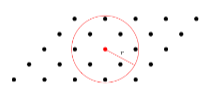
\includegraphics[width = 4cm]{media/sfera di amming.png}
                \label{sfera di Hamming}
                \end{figure}
                Se adottiamo un ricevitore ML, il numero massimo di errori che il codice $\mathcal{C}(k,n)$ é in grado di correggere é il massimo raggio $t$ per cui le sfere centrate nelle 
                parole di codice di $\mathcal{C}(k,n)$ sono tutte tra loro disgiunte.
            \paragraph{Capacitá di correggere errori (Error Correction):}
                \subparagraph{Teorema:}\begin{sloppypar}
                   Un codice lineare a blocco puó correggere fino a ${t_{max} = \left\lfloor \frac{d_{min}-1}{2} \right\rfloor}$ errori: $2t_{max}+1 \leq d_{min} \leq 2t_{max}+2$.
                \end{sloppypar}
                    
                \begin{sloppypar}
                    La condizione per cui le sfere di raggio $t$ che circondano le parole di codice siano disgiunte é che ${2t_{max} < d_{min}\Rightarrow t_{max} < \frac{d_min}{2}}$.
                    Altrimenti se fosse  ${2t_{max} \geq d_{min}}$ ci sarebbero almeno die parole $x_1$ e $x_2$ la cui distanza ${d_H(x_1,x_2) = d_{min} < 2t_{max} }$ e le que sfere di raggio
                    $t$ avrebbero almno un unto in comune.
                \end{sloppypar}
                
                \begin{sloppypar}
                    Consideriamo il codice $\mathcal{C}(k,n)$ che ha una certa $d_{min}$ e $t_{max}$ tale che ${2t_{max}+1 \leq d_{min}}$. Sia $x\in\mathcal{C}(k,n)$ la parola trasmessa,
                    ${y = x+e}$ la corrispondente sequenza di $n$ bit ricevuta e $c\in\mathcal{C}(k,n)$ un'altra generica parola di codice. Grazie alla disuguaglianza triangolare ho:
                    \[
                        d_H(x,y) + d_H(c,y) \geq d_H(x,c) \Rightarrow d_H(c,y) \leq d_H(x,c) - d_H(x,y)  
                    \]
                    per ipotesi ho anche:
                    \[
                        d_H(x,c) \geq d_{min} \geq 2t_{max}+1 
                    \]
                    Supponiamo che il canale introduca un certo numero di errori ${t\leq} t_{max}$, cosí da avere $d_H(x,y) = t$:
                    \[
                        d_H(c,y) \geq 2t_{max}+1 -t > t_{max} \geq t = d_H(x,y)   
                    \]   
                \end{sloppypar}
                
    \subsection{Codici di Hamming}
        I codici di Hamming $\mathcal{C}_H(m)$ sono definiti a partire da un parametro: $m \geq 2$
        \[
            n = 2^m-1,\ k = 2^m-m-1 = n-m
        \]
        \subparagraph{Matrice di controllo di paritá:} per definizione la matrice $H \in (n-k)\times n$, ma per i codici di Hamming la matrice $H$ ha dimensione:
        $H \in m\times (2^m-1)$.

        \subparagraph{Matrice di paritá:} Per un codice di Hamming sistematico la matrice di parità $P\in k \times m$ viene costruita cosí che le colonne di $H = [P^T,I_{n-k}]$
        siano tutte le possibili $2^m-1$ combinazioni di $m$ bit (esclusa la $n-upla$ di tutti 0)

        \subsubsection{Il codice $\mathcal{C}_H(2)$}
            \begin{sloppypar}
                Il codice a ripetizione ${R=\frac{1}{3}}$ con ${m=2\Rightarrow n=3,\ k=1}$ ha come matrice di controllo di paritá $H$:
                \[
                    H = \begin{bmatrix}
                            1  & 1 & 0 \\
                            1  & 0 & 1 \\
                        \end{bmatrix} 
                \]
                Che é la matrice corrispondente a un codice di Hamming $\mathcal{C}_H(2)$, poiché rappresenta tutte le possibili combinazioni di 2 bit
            \end{sloppypar}

        \subsubsection{Il codice $\mathcal{C}_H(3)$}
        \begin{gather}
            m=3,\ n=7,\ k=4,\ R=\frac{4}{7} \nonumber \\
            H = \begin{bmatrix}
                1 & 0 & 1 & 0 & 1 & 0 & 1\\
                0 & 1 & 1 & 0 & 0 & 1 & 1\\
                0 & 0 & 0 & 1 & 1 & 1 & 1
            \end{bmatrix}  \nonumber
        \end{gather}
        Posso ricavare la matrice generatrice $G$ scrivendo la matrice $H$ come se l'avessi ottenuta da una matrice $G\in k \times n$ di un codice sistematico (\ref{Matrice di controllo di parita}):
        \[
            H = [P^T,I_{n-k}] =\begin{bmatrix}
                                 1  & 1 & 0 & 1 & | & 1  & 0 & 0\\
                                 1  & 0 & 1 & 1 & | & 0  & 1 & 0\\
                                 0  & 1 & 1 & 1 & | & 0  & 0 & 1
                            \end{bmatrix} 
        \]
        La cui matrice generatrice con $I \in k \times k$ é:
        \[
            G = [I_{k},P] =\begin{bmatrix}
                                 1  & 0 & 0 & 0 & | & 1  & 1 & 0\\
                                 0  & 1 & 0 & 0 & | & 1  & 0 & 1\\
                                 0  & 0 & 1 & 0 & | & 0  & 1 & 1\\
                                 0  & 0 & 0 & 1 & | & 1  & 1 & 1
                            \end{bmatrix} 
        \]
        Possiamo vedere come la matrice di paritá faccia conrolli su combinazioni diverse di bit in ingresso $p = uP$:
        \begin{gather}
            p_1 = u_1+u_2+u_4 \nonumber\\
            p_2 = u_1+u_3+u_4 \nonumber\\
            p_3 = u_2+u_3+u_4 \nonumber
        \end{gather}
        Il vettore di uscita dal codificatore sará quindi $x = uG = [u,p_1,p_2,p_3]$, tale matrice di paritá ci permette di aumentare la distanza di Hamming
        tra le parole
        \subparagraph{Distanza minima:} La distanza minima di un qualsiasi codice di Hamming $\mathcal{C}_H(m)$ é $d_{min}(\mathcal{C}_H(m)) = 3$.

        \noindent Dimostrazione: 
        \begin{enumerate}
            \item {
                $d_{min} = \underset{x\in\mathcal{C}}{\min}\ w(x)$  
            }
            \item {
                $x\in\mathcal{C}\ se\ xH^T= 0$ e le colonne di $H$ sono tutte le possibili combinazioni dei bit $m$ bit
            }
        \end{enumerate}
        Perché $3$ é il numero minimo di colonne che mi permette di ottenere $0$ ($2$), quindi $d_{min}(\mathcal{C}_H(m)) = 3$.
        
        %Ne consegue che aumentando il numero di bit trasmessi diminuisco la ridondanza, ma la mia distanza di Hamming rimane sempre la stessa.
    \subsection{Decodifica per codici a blocco}
        Dato il vettore ricevuto:
        \[
            y = x+e
        \]
        Il decisore ottimo selezione la parola di codice $\hat{x}$:
        \[
            \hat{x} = \arg \underset{x\in\mathcal{C}}{\max}\ P(y|x) = \arg \underset{x\in\mathcal{C}}{\min}\ d_H(y,x)   
        \]
        Per ottenere $\hat{x}$ é necessario fare $2^k$ confronti tra il vettore ricevuto $y$ e tutte le parole di codice $\mathcal{C}(k,n)$, 
        la complessitá cresce esponenzialmente con $k$.

        Un approccio alternativo é quello di osservare il vettore errore e la probabilitá condizionata:
        \begin{gather}
            y= x+e \Rightarrow x = y+e,\ e = y-x\nonumber\\
            P(x|y) = P(x+e|x) = P(e|y+e\in\mathcal{C})\nonumber
        \end{gather}
        Posso ottenera la stima di $x$ come:
        \[
            \hat{x} = \arg \underset{x\in\mathcal{C}}{\max}\ P(y|x) =y+ \arg \underset{e}{\max}\ P(e|y+e\in\mathcal{C})   
        \]
        Invece di stimare $\hat{x}$ si stima il vettore $\hat{e}$ piú probabile
        \begin{align}
            \hat{e} &= \arg \underset{e}{\max}\ P(e|y+e\in\mathcal{C}) = \arg \underset{e|y+e\in\mathcal{C}}{\max}\ p^{w(e)}(1-p)^{n-w(e)} \nonumber \\
                    &= \arg \underset{e|y+e\in\mathcal{C}}{\max}\ \left(\frac{1-p}{p}\right)^{-w(e)} = \arg \underset{e|y+e\in\mathcal{C}}{\min}\ w(e)  \nonumber 
        \end{align}
        La decodifica sceglie tra tutti i possibili vettori errore $e$ tali che $y+e\in\mathcal{C}$ quello che ha il peso di Hamming minimo, cioé il minimo numero di 
        errori (Massima Verosomiglianza). Una volta stimato $\hat{e}$:
        \[
            \hat{x} = y-\hat{e} = y+\hat{e} = x+(\hat{e}+e)=
            \begin{cases}
                x &se\ \hat{e} = e\nonumber\\    
                x_1\neq x &se\ \hat{e} \neq e\nonumber    
            \end{cases}     
        \]
        \subsubsection{Coset}
            Sia $\mathcal{C}(k,n)$ un codice a blocco e sia $v\in \mathcal{V}_n$ un vettore di $n$ cifre binarie, si definisce $coset$ di
            $\mathcal{C}(k,n)$ individuato da $v$ l'insieme:
            \[
                C_v = C+v=\{ x+v: x\in\mathcal{C} \}
            \]
        \subsubsection{Propietá dei coset}
            \begin{enumerate}
                \item {Qualsiasi vettore in $\mathcal{V}_n$ appartiene a un coset di $\mathcal{C}(k,n)$}
                \item {Ciascun coset contiene $2^k$ elementi}
                \item {Due coset o sono coincidenti o hanno intersezione nulla}
                \item {Ci sono $2^{n-k}$ coset distinti}
                \item {Se $v_1$ e $v_2$ appartengono all ostesso coset, $v_1 + v_2 \in \mathcal{C}(k,n)$ é una parola di codice}
            \end{enumerate}
            \paragraph{Esempio di coset:}
                \begin{sloppypar}
                    Sia ${\mathcal{C}(2,3) = \{000,101,010,111\}}$. I coset di ${\mathcal{C}(2,3)}$: 
                \end{sloppypar}
                \begin{align}
                    \mathcal{C} + 000 = \{000,101,010,111\} = \mathcal{C}_0 \\
                    \mathcal{C} + 001 = \{001,100,011,110\} = \mathcal{C}_1 \\
                    \mathcal{C} + 010 = \{010,111,000,101\} = \mathcal{C}_0 \\
                    \mathcal{C} + 011 = \{011,110,001,100\} = \mathcal{C}_1 \\
                    \mathcal{C} + 100 = \{100,001,110,011\} = \mathcal{C}_1 \\
                    \mathcal{C} + 101 = \{101,000,111,010\} = \mathcal{C}_0 \\
                    \mathcal{C} + 110 = \{110,011,100,001\} = \mathcal{C}_1 \\
                    \mathcal{C} + 111 = \{111,010,101,000\} = \mathcal{C}_0 
                \end{align}
                Il numero di coset é $2^{n-k} = 2^{3-2} =2$.

            Si possono applicare i coset per la decodifica: $y=x+e$ dalla definizione di coset discende che i vettori $e$ e $y$
            appartengono allo stesso coset $\mathcal{C}_y$ e che i coset $\mathcal{C}_e$ e $\mathcal{C}_x$ sono coincidenti. Grazie alla propietá
            dei coset la somma di qualsiasi elemento di $\mathcal{C}_y$ con $y$ individua una parola di codice. Il vettore $e$ va scelto fre gli elementi
            di $\mathcal{C}_y$, la regola di decisione diveta:
            \[
                \hat{e} = \arg \underset{e}{\max}\ P(e|y+e\in\mathcal{C}) = \arg \underset{e\in\mathcal{C}_y }{\max}\ P(e) =\arg \underset{v\in\mathcal{C}_y }{\max}\ w(v)
            \] 
            Tra tutti i $2^k$ possibili vettori di $\mathcal{C}_y$, il principio di massima verosomiglianza dice che devo scegliere quello di peso minimo.
        \subsubsection{Algoritmo di decodifica}
            \begin{enumerate}
                \item Avendo ricevuto il vettore $y$ si trova un coset di appartenenza $\mathcal{C}_y$.
                \item {Si identifica il coset leader, la parola di peso minimo del coset $\mathcal{C}_y$, che é anche la parola di peso minimo del 
                coset di $\mathcal{C}_e$.}
                \item Il coset leader é la stima del vettore di errore $\hat{e}$
            \end{enumerate}
            \paragraph{Esempio di decodifica utilizzando i coset:}
                    Sia ${\mathcal{C}(2,4) = \{0000,1011,0101,1110\}}$ con $d_{min} = 2$, ho i coset: 
                \begin{align}
                    \mathcal{C} + 0000 = \{0000,1011,0101,1110\} \\
                    \mathcal{C} + 0001 = \{0001,1010,0100,1111\} \\
                    \mathcal{C} + 0010 = \{0010,1001,0111,1100\} \\
                    \mathcal{C} + 1000 = \{1000,0011,1101,0110\} 
                \end{align}
                Il numero di coset é $2^{n-k} = 2^{4-2} =4$. Il coset (2) non so quale coset leader scegliere hanno lo stesso peso di Hamming, ci
                troviamo in questo poiché la $d_{min}$ é molto bassa e ho il $50\%$ di possibilitá di sbagliare se il codice ricevuto capita in questo coset.
                Decodifichiamo:
                \begin{itemize}
                    \item {$y=[1101]\Rightarrow y\in (4),\text{coset leader:} [1000]\ \hat{x}=y+1000=0101$}
                    \item {$y=[1111]\Rightarrow y\in (2),\text{coset leader:} [0001] \vee [0100] \ \hat{x}=y+0001=1110$}
                \end{itemize}
        \subsubsection{Decodifica mediante sindrome}
            Si definisce sindrome di $y$ il vettore $s$ ottenuto dal prodotto di $y$ con la matrice di controllo di paritá:
            \[
                s = yH^T = (x+e)H^T = xH^T+eH^T = eH^T    
            \]
            \paragraph{Propietá:}
                \begin{itemize}
                    \item {
                        Tutti i membri di uno stesso coset hanno la stessa sindrome
                    }
                    \item {
                        $s \in 1 \times (n-k)$
                    }
                    \item {
                        Le $2^{n-k}$ sindromi sono associate ai $2^n-k$ diversi coset del codice $\mathcal{C}(k,n)$
                    }
                    \item {
                        Ciascuna sindrome é associata ai $2^k$ pattern di errore apparteenti allo stesso coset.
                    }
                \end{itemize}
            \paragraph{Procedura di decodifica:}
                \begin{enumerate}
                    \item {Calcola la sindrome $s = yH^T$}
                    \item {Associa la sindrome al coset leader corrispondente $s\rightarrow e_{CL}(s)$}
                    \item {Corregge l'errore sommando il coset leader alla $n-upla\ y$}
                \end{enumerate}
                La parola $\hat{x}$ é una parola di codice:
                \[
                    \hat{x}H^T= (y+e_{CL}(s))H^T = s+s =0   
                \]
                e per costruzione la parola di codice $\hat{x}$ minimizza la distanza di Hamming da $y$
        \subsubsection{Decodifica a sindrome: Codici di Hamming $m=3$}
            \begin{sloppypar}
                Il codice ha $d_{min} = 3$ ed é in grado di correggere esattamente un errore: ${t_{max} = \left\lfloor \frac{d_{min}-1}{2}\right\rfloor = 1}$. Si sceglie la matrice $H$
                in maniera che la tabella di decodifica associ alla sindrome il pattern di errore a peso 1 in cui il bit
                messo a 1 sia nella posizione corrispondente alla conversione della sindrome in decimale.
            \end{sloppypar}
            \begin{table}[H]
                \subfloat[Codice non sistematico]{
                    \begin{tabular}{cc}
                        \hline
                        Sindrome  & Coset Leader  \\ \hline
                        {[}000{]} & {[}0000000{]} \\
                        {[}100{]} & {[}1000000{]} \\
                        {[}010{]} & {[}0100000{]} \\
                        {[}110{]} & {[}0010000{]} \\
                        {[}001{]} & {[}0001000{]} \\
                        {[}101{]} & {[}0000100{]} \\
                        {[}011{]} & {[}0000010{]} \\
                        {[}111{]} & {[}0000001{]} \\ \hline
                        \end{tabular}
                }
                \hfill
                \subfloat[Codice sistematico]{
                    \begin{tabular}{cc}
                        \hline
                        Sindrome  & Coset Leader  \\ \hline
                        {[}000{]} & {[}0000000{]} \\
                        {[}100{]} & {[}0000100{]} \\
                        {[}010{]} & {[}0000010{]} \\
                        {[}110{]} & {[}1000000{]} \\
                        {[}001{]} & {[}0000001{]} \\
                        {[}101{]} & {[}0100000{]} \\
                        {[}011{]} & {[}0010000{]} \\
                        {[}111{]} & {[}0001000{]} \\ \hline
                    \end{tabular}
                }
            \end{table}
        \subsubsection{Esempio di decodifica}
            Un codice lineare a blocchi ha la seguente matrice di controllo di parità:
            \[
                H=
                    \begin{bmatrix}
                    1 & 0 & 1 & 1 & 0 & 0\\
                    1 & 1 & 0 & 0 & 1 & 0\\
                    0 & 1 & 1 & 0 & 0 & 1
                    \end{bmatrix}  
            \]  
            \begin{enumerate}
                \item {Determinare la matrice generatrice:
                
                }
                \item {Decodificare la parola $y = [110110]$ ed identificare la parola di codice trasmessa:
                
                }
            \end{enumerate}




































    \section{Formulario}
    \subsection{Trigonometria}\label{Trigonometria}
        \begin{enumerate}
            \item {
                $\sin^2(\alpha) + \cos^2(\alpha) = 1$
            }
            \item {
                $\cos(\alpha)=\pm\frac{1}{\sqrt{1+\tan^2(\alpha)}}$
            }
            \item {
                $\sin(\alpha)=\pm\frac{\tan(\alpha)}{\sqrt{1+\tan^2(\alpha)}}$
            }
            \item {
                $sinc(\alpha)\triangleq\frac{\sin(\pi\alpha)}{\pi\alpha}$ 
                É un $\sin(\alpha)$ smorzato secondo $\frac{1}{x}$ che si annulla in $k\pi: k\in\mathbb{Z}$
                \begin{figure}[htp]
                    \centering
                    
\includegraphics[width=4cm]{media/uwu.png}
                    \caption{grafico $sinc(\alpha)$}
                    \label{fig:grafico sinc}
                \end{figure}
            }
        \end{enumerate}
        \subsubsection{Formule di addizione}\label{Trigonometria_Addizione}
            \begin{enumerate}
                \item {
                    $\cos(\alpha \pm \beta) = \cos(\alpha)\cos(\beta) \mp \sin(\alpha)\sin(\beta)$
                }
                \item {
                    $\sin(\alpha \pm \beta) = \sin(\alpha)\cos(\beta) \pm \sin(\beta)\cos(\alpha)$
                }
                \item {
                    $\tan(\alpha \pm \beta) = \frac{\tan(\alpha) \pm \tan(\beta)}{1 \mp \tan(\alpha)\tan(\beta)} $
                }
            \end{enumerate}
        \subsubsection{Formule di duplicazione}\label{Trigonometria_Duplicazione}
            \begin{enumerate}
                \item {
                    $\sin(2\alpha) =2\sin(\alpha)\cos(\alpha)$ 
                }
                \item {
                    $
                        \cos(2\alpha)
                        \begin{cases}
                            \cos^2(\alpha) - \sin^2(\alpha) \\
                            2\cos^2(\alpha)-1\\
                            1-2\sin^2(\alpha)
                        \end{cases}
                    $
                }
                \item {
                    $\tan(2\alpha) =\frac{2\tan(\alpha)}{1-\tan^2(\alpha)}$ 
                }
            \end{enumerate}
            \subsubsection{Formule di bisezione}\label{Trigonometria_Bisezione}
                \begin{enumerate}
                    \item {
                        $\sin(\frac{\alpha}{2}) =\pm\sqrt{\frac{1-\cos(\alpha)}{2}}$ 
                    }
                    \item {
                        $\cos(\frac{\alpha}{2}) =\pm\sqrt{\frac{1+\cos(\alpha)}{2}}$ 
                    }
                    \item {
                        $
                            \tan(\frac{\alpha}{2})
                            \begin{cases}
                                \sqrt{\frac{1-\cos(\alpha)}{1+\cos(\alpha)}} \\
                                \frac{1-\cos(\alpha)}{\sin(\alpha)}\\
                                \frac{\sin(\alpha)}{1+\cos(\alpha)}
                            \end{cases}
                        $
                    }
                \end{enumerate}
    \subsection{Segnali Comuni}\label{Segnali Comuni}

    \printindex
\end{document}